\documentclass[Thesis]{subfiles}
\begin{document}
%\setkeys{Gin}{draft=false}

\chapter{Discrete uniformization of Riemann surfaces}
\label{chp:uniformization}

\section{Introduction}

\begin{figure}
\centering
\resizebox{0.9\textwidth}{!}{
\includegraphics[height=10cm]{introduction/genus0_image.pdf}
\quad
\includegraphics[height=10cm]{introduction/genus0_domain.pdf}
}
\resizebox{0.9\textwidth}{!}{
\includegraphics[height=10cm]{introduction/genus1_image.pdf}
\quad    
\raisebox{0.5cm}{\includegraphics[height=9cm]{introduction/genus1_domain.pdf}}
}
\resizebox{0.9\textwidth}{!}{
\includegraphics[height=10cm]{introduction/genus3_image.pdf}
\quad   
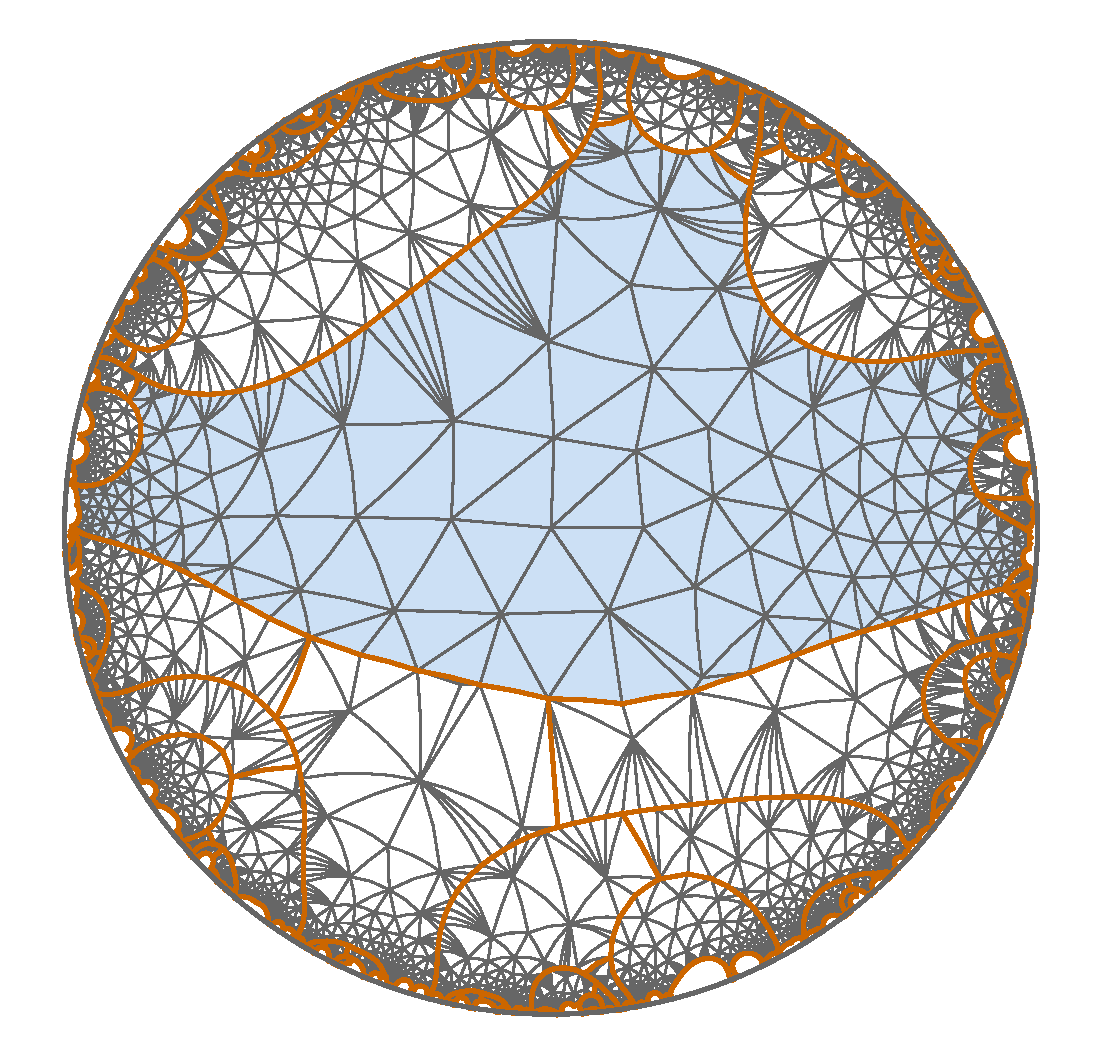
\includegraphics[height=10cm]{introduction/genus3_domain.pdf}
}
\setstretch{0.0}{\scriptsize\tt data/introduction/genus\{0/1/3\}\_data.xml} 
\caption{
Uniformization of compact Riemann surfaces. 
The uniformization of spheres is treated in
Section~\ref{sec:spheres}. Tori are covered in
Section~\ref{sec:tori}, and Section~\ref{sec:higher_genus} is
concerned with surfaces of higher genus.
}
\label{fig:intro_uniformization}
\end{figure}

In this chapter we investigate various applications of discrete conformal maps. 
It is a joint effort of Alexander Bobenko, Boris Springborn, and the author. Most of its content is also available in the article~\cite{BobSechSpr}.
We build upon the work of Bobenko, Pinkall, and Springborn~\cite{BPS2015:dconf} and Springborn, Schr\"{o}der, and Pinkall~\cite{Springborn2008}. 
We present examples for uniformizations of Riemann surfaces of genus $0$, $1$, and $g>1$ based on this theory, see Figure~\ref{fig:intro_uniformization}.

The notion of discrete conformal equivalence for polyhedral surfaces
is based on a simple definition: Two polyhedral surfaces are
discretely conformally equivalent if the edge lengths are related by
scale factors assigned to the vertices. It leads to a surprisingly
rich theory~\cite{Luo2004:Yamabe, BPS2015:dconf, Luo-Uniformization, Luo-Uniformization_II}.

We extend the notion of discrete conformal equivalence from
triangulated surfaces to polyhedral surfaces with faces that are
inscribed in circles. The basic definitions and their immediate
consequences are discussed in Section~\ref{sec:basic_definitions}. 

In Section~\ref{sec:vari-princ}, we generalize a variational principle
for discretely conformally equivalent
triangulations~\cite{BPS2015:dconf} to the polyhedral setting. This
variational principle is the main tool for all our numerical
calculations. It is also the basis for our uniqueness proof for
discrete conformal mapping problems
(Theorem~\ref{thm:uniqueness}). 

Section~\ref{sec:quadrangulations} is concerned with the special case
of quadrilateral meshes. We discuss the emergence of
orthogonal circle patterns, a peculiar necessary condition for the
existence of solutions for boundary angle problems, and we extend the
method of constructing discrete Riemann maps from triangulations to
quadrangulations.

In Section~\ref{sec:multiply_connected}, we briefly discuss discrete
conformal maps from multiply connected domains to circle domains, and
special cases in which we can map to slit domains. 

Section~\ref{sec:spheres} deals with conformal mappings onto the
sphere. We generalize the method for triangulations to
quadrangulations, and we explain how the spherical version of the
variational principle can in some cases be used for numerical
calculations although the corresponding functional is not convex.

Section~\ref{sec:tori} is concerned with the uniformization of tori,
i.e., the representation of Riemann surfaces as a quotient space of
the complex plane modulo a period lattice. We consider Riemann
surfaces represented as immersed surfaces in $\R^{3}$, and as elliptic
curves. We conduct numerical experiments to test the conjectured
convergence of discrete conformal maps. We consider the difference
between the true modulus of an elliptic curve (which can be calculated
using hypergeometric functions) and the modulus determined by discrete
uniformization, and we estimate the asymptotic dependence of this
error on the number of vertices.

In Section~\ref{sec:higher_genus}, we consider the Fuchsian
uniformization of Riemann surfaces represented in different forms. We
consider immersed surfaces in $\R^{3}$ (and $S^{3}$), hyperelliptic
curves, and Riemann surfaces represented as a quotient of $\Chat$
modulo a classical Schottky group. That is, we convert from Schottky
uniformization to Fuchsian uniformization. The Section ends with two
extended examples demonstrating, among other things, a remarkable
geometric characterization of hyperelliptic surfaces due to Schmutz
Schaller.

This text is accompanied by a compact disk which contains the data for all of the examples presented in this part of the work. 
Where applicable, we give the path to the data on the disk directly under the corresponding figure.
We describe the usage of the software and the XML data format that was used to create all the results in Chapter~\ref{chp:conformallab}.

\section{Discrete conformal equivalence of cyclic polyhedral surfaces}
\label{sec:basic_definitions}

\subsection{Cyclic polyhedral surfaces }

A \emph{euclidean polyhedral surface} is a surface obtained from
gluing euclidean polygons along their edges. (A \emph{surface} is a
connected two-dimensional manifold, possibly with boundary.)  In other
words, a euclidean polyhedral surface is a surface equipped with,
first, an intrinsic metric that is flat except at isolated points
where it has cone-like singularities, and, second, the structure of a
CW complex with geodesic edges. The set of vertices contains all
cone-like singularities. If the surface has a boundary, the boundary
is polygonal and the set of vertices contains all corners of the
boundary.

\emph{Hyperbolic polyhedral surfaces} and \emph{spherical polyhedral
surfaces} are defined analogously. They are glued from polygons in
the hyperbolic and elliptic planes, respectively. Their metric is
locally hyperbolic or spherical, except at cone-like singularities.

We will only be concerned with polyhedral surfaces whose faces are all
cyclic, i.e., inscribed in circles. We call them \emph{cyclic
polyhedral surfaces}. More precisely, we require the polygons to be
cyclic before they are glued together. It is not required that the
circumcircles persist after gluing; they may be disturbed by cone-like
singularities. A polygon in the hyperbolic plane is considered cyclic
if it is inscribed in a curve of constant curvature. This may be a
circle (the locus of points at constant distance from its center), a
horocycle, or a curve at constant distance from a geodesic.

A \emph{triangulated surface}, or \emph{triangulation} for short, is a
polyhedral surface all of whose faces are triangles.  All
triangulations are cyclic.

\subsection{Notation}
\label{sec:notation}

We will denote the sets of vertices, edges, and faces of a CW complex~$\Sigma$ by $V_{\Sigma}$, $E_{\Sigma}$, and $F_{\Sigma}$, and we will often omit the subscript when there is no danger of confusion.
For notational convenience, we require all CW complexes to be \emph{strongly regular}. 
This means that we require that faces are not glued to themselves along edges or at vertices, that two faces are not glued together along more than one edge or one vertex, and that edges have distinct end-points and two edges have at most one endpoint in common. 
This allows us to label edges and faces by their vertices. 
We will write $\mathit{ij}\in E$ for the edge with vertices $i,j\in V$ and $\mathit{ijkl}\in F$ for the face with vertices $i,j,k,l\in V$. 
We will always list the vertices of a face in the correct cyclic order, so that for example the face $\mathit{ijkl}$ has edges $\mathit{ij}$, $\mathit{jk}$, $\mathit{kl}$, and $\mathit{li}$.
The only reason for restricting our discussion to strongly regular CW complexes is to be able to use this simple notation. 
Everything we discuss applies also to general CW complexes.

% We will denote the sets of boundary vertices and edges by $\Vbdy$ and
% $\Ebdy$, and the complementary sets of interior vertices and edges by
% $\Eint$ and $\Vint$. In some formulas we need to iterate over directed
% edges.  We denote the set of directed edges by $\vect{E}$.  For each
% edge $\mathit{ij}\in E$ the set $\vect{E}$ contains two directed edges
% $\mathit{ij}\in \vect{E}$ and $\mathit{ji}\in \vect{E}$.

\subsection{Discrete metrics}
\label{sec:discrete_metrics}

The \emph{discrete metric} of a euclidean (or hyperbolic or spherical)
cyclic polyhedral surface $\Sigma$ is the function
$\ell:E_{\Sigma}\rightarrow\R_{>0}$ that assigns to each edge ${\it ij}
\in E_{\Sigma}$ its length $\ell_{\it ij}$.  It satisfies the polygon
inequalities (one side is shorter than the sum of the others):
\begin{equation}
\label{eq:polygon_ineq}
\left.
\quad
\begin{aligned}
-\ell_{i_{1}i_{2}}+\ell_{i_{2}i_{3}}+&\ldots+\ell_{i_{n-1}i_{n}}
>0\\
\ell_{i_{1}i_{2}}-\ell_{i_{2}i_{3}}+&\ldots+\ell_{i_{n-1}i_{n}}
>0\\
&\vdots\\
\ell_{i_{1}i_{2}}+\ell_{i_{2}i_{3}}+&\ldots-\ell_{i_{n-1}i_{n}}
>0
\end{aligned}
\quad
\right\}
\quad
\text{for all $i_{1}i_{2}\ldots i_{n}\in F_{\Sigma}$}
\end{equation}
In the case of spherical polyhedral surfaces, we also require that
\begin{equation}
  \label{eq:polygon_ineq_spherical}
  \ell_{i_{1}i_{2}}+\ell_{i_{2}i_{3}}+\ldots+\ell_{i_{n-1}i_{n}}
<2\pi.
\end{equation}

The polygon inequalities~\eqref{eq:polygon_ineq} are necessary and
sufficient for the existence of a unique cyclic euclidean polygon and
a unique cyclic hyperbolic polygon with the given edge
lengths. Together with inequality~\eqref{eq:polygon_ineq_spherical}
they are necessary and sufficient for the existence of a unique cyclic
spherical polygon. For a new proof of these elementary geometric
facts, see~\cite{KSS15}. Thus, a discrete metric determines the geometry of
a cyclic polyhedral surface:

\begin{propdef}
  \label{def:sigma_ell_g}
  If $\Sigma$ is a surface with the structure of a CW~complex and a
  function $\ell:E_{\Sigma}\rightarrow\R_{>0}$ satisfies the polygon
  inequalities~\eqref{eq:polygon_ineq}, then there is a unique
  euclidean cyclic polyhedral surface and also a unique hyperbolic
  cyclic polyhedral surface with CW~complex~$\Sigma$ and discrete
  metric~$\ell$. If $\ell$ also satisfies the
  inequalities~\eqref{eq:polygon_ineq_spherical}, then there is a
  unique spherical cyclic polyhedral surface with CW~complex~$\Sigma$
  and discrete metric~$\ell$. 

  We will denote the euclidean, hyperbolic, and spherical polyhedral
  surface with CW~complex $\Sigma$ and discrete metric $\ell$ by\/
  $(\Sigma,\ell)_{\euc}$, $(\Sigma,\ell)_{\hyp}$, and\/
  $(\Sigma,\ell)_{\sph}$, respectively.
\end{propdef}

\subsection{Discrete conformal equivalence}
\label{sec:discr-conf-equiv}

We extend the definition of discrete conformal equivalence from
triangulations~\cite{Luo2004:Yamabe,BPS2015:dconf} to cyclic
polyhedral surfaces in a straightforward way
(Definition~\ref{def:dconf}). While some aspects of the theory carry
over to the more general setting (e.g., M{\"o}bius invariance,
Proposition~\ref{prop:Moebius_inv}), others do not, like the
characterization of discretely conformally equivalent triangulations
in terms of length cross-ratios (Section~\ref{sec:triangulations}). We
will discuss similar characterizations for polyhedral surfaces with
$2$-colorable vertices and the particular case of quadrilateral faces
in Sections~\ref{sec:even_cycles} and~\ref{sec:quads}.

We define discrete conformal equivalence only for polyhedral surfaces
that are combinatorially equivalent (see
Remark~\ref{rem:change_combi}). Thus, we may assume that the surfaces
share the same CW complex~$\Sigma$ equipped with different metrics
$\ell$, $\ellt$.

\begin{definition}
  \label{def:dconf}
  \emph{Discrete conformal equivalence} is an equivalence relation on
  the set of cyclic polyhedral surfaces defined as follows:
  \begin{compactitem}[$\bullet$]
  \item Two \emph{euclidean} cyclic polyhedral surfaces
    $(\Sigma,\ell)_{\euc}$ and $(\Sigma,\ellt)_{\euc}$ are
    \emph{discretely conformally equivalent} if there exists a
    function $u:V_{\Sigma}\rightarrow\R$ such that
    \begin{equation}
      \label{eq:tilde_ell_euc}
      \ellt_\mathit{ij}=e^{\frac{1}{2}(u_{i}+u_{j})}\ell_\mathit{ij}.
    \end{equation}
  \item Two \emph{hyperbolic} cyclic polyhedral surfaces
    $(\Sigma,\ell)_{\hyp}$ and $(\Sigma,\ellt)_{\hyp}$ are \emph{discretely
      conformally equivalent} if there exists a function
    $u:V_{\Sigma}\rightarrow\R$ such that
    \begin{equation}
      \label{eq:tilde_ell_hyp}
      \sinh\Big(\frac{\ellt_\mathit{ij}}{2}\Big)
      = e^{\frac{1}{2}(u_{i}+u_{j})}\,
      \sinh\Big(\frac{\ell_\mathit{ij}}{2}\Big).
    \end{equation}
  \item Two \emph{spherical} cyclic polyhedral surfaces
    $(\Sigma,\ell)_{\sph}$ and $(\Sigma,\ellt)_{\sph}$ are \emph{discretely
      conformally equivalent} if there exists a function
    $u:V_{\Sigma}\rightarrow\R$ such that
    \begin{equation}
      \label{eq:tilde_ell_sph}
      \sin\Big(\frac{\ellt_\mathit{ij}}{2}\Big)
      = e^{\frac{1}{2}(u_{i}+u_{j})}\,
      \sin\Big(\frac{\ell_\mathit{ij}}{2}\Big).
    \end{equation}
  \end{compactitem}

We will also consider mixed versions: 
\begin{compactitem}[$\bullet$]
\item A euclidean cyclic polyhedral surface $(\Sigma,\ell)_{\euc}$ and a
  hyperbolic cyclic polyhedral surface $(\Sigma,\ellt)_{\hyp}$ are
  discretely conformally equivalent if
  \begin{equation}
    \label{eq:tilde_ell_hyp_euc}
    \sinh\Big(\frac{\ellt_\mathit{ij}}{2}\Big)
    = e^{\frac{1}{2}(u_{i}+u_{j})}\ell_\mathit{ij}.
  \end{equation}
\item A euclidean cyclic polyhedral surface $(\Sigma,\ell)_{\euc}$ and a spherical cyclic
  polyhedral surface $(\Sigma,\ellt)_{\sph}$ are discretely conformally
  equivalent if
  \begin{equation}\label{eq:tilde_ell_sph_euc}
    \sin\Big(\frac{\ellt_\mathit{ij}}{2}\Big)
    = e^{\frac{1}{2}(u_{i}+u_{j})}\ell_\mathit{ij}.
  \end{equation}
\item A hyperbolic cyclic polyhedral surface $(\Sigma,\ell)_{\hyp}$ and a spherical cyclic
  polyhedral surface $(\Sigma,\ellt)_{\sph}$ are discretely conformally
  equivalent if
  \begin{equation}\label{eq:tilde_ell_sph_hyp}
    \sin\Big(\frac{\ellt_\mathit{ij}}{2}\Big)
    = e^{\frac{1}{2}(u_{i}+u_{j})}\sinh\Big(\frac{\ell_\mathit{ij}}{2}\Big).
  \end{equation}
\end{compactitem}
\end{definition}

\begin{remark}
  \label{rem:chords}
  Note that relation~\eqref{eq:tilde_ell_sph} for spherical edge
  lengths is equivalent to relation~\eqref{eq:tilde_ell_euc} for the
  euclidean lengths of the chords in the ambient $\R^{3}$ of the
  sphere (see Figure~\ref{fig:geometries}, left).
  \begin{figure}
    \begin{minipage}[b]{0.6\linewidth}
      \centering \resizebox{\textwidth}{!}{
        \input{figures/geometries/spherical.pdf_t}
        \input{figures/geometries/hyperbolic.pdf_t} }
      \caption{Spherical and hyperbolic chords.}
      \label{fig:geometries}
    \end{minipage}
    \hfill
    \begin{minipage}[b]{0.33\linewidth}
      \centering
      \input{figures/lengthcrossratio.pdf_t}
      \caption{Length cross-ratio.}
      \label{fig:lcr}
    \end{minipage}
  \end{figure}
  Likewise, relation~\eqref{eq:tilde_ell_hyp} for hyperbolic edge
  lengths is equivalent to~\eqref{eq:tilde_ell_euc} for the euclidean
  lengths of the chords in the ambient $\R^{2,1}$ of the hyperboloid
  model of the hyperbolic plane (see Figure~\ref{fig:geometries},
  right).
\end{remark}

\begin{remark}
  \label{rem:change_combi}
  For triangulations, the definition of discrete conformal equivalence
  has been extended to meshes that are not combinatorially
  equivalent~\cite[Definition 5.1.4]{BPS2015:dconf}
  \cite{Luo-Uniformization, Luo-Uniformization_II}. It is not
  clear whether or how the following definitions for cyclic polyhedral
  surfaces can be extended to combinatorially inequivalent CW
  complexes.
\end{remark}

% \begin{remark*}[Orientation]
%   We need and will only consider oriented surfaces because the
%   solutions of the conformal mapping problems that we treat are
%   sufficiently unique. The situation is like in the classical smooth
%   case: While one could consider the uniformization of nonorientable
%   Riemann surfaces (by allowing anticonformal chart transition
%   functions and discrete groups containing orientation reversing
%   M\"obius transformations), this would not lead to anything
%   essentially new: Due to uniqueness, the uniformization of an
%   unorientable surface lifts to the oriented double cover.
% \end{remark*}

The discrete conformal class of a cyclic polyhedral surface embedded
in $n$-dimensional euclidean space is invariant under M{\"o}bius
transformations of the ambient space:

\begin{proposition}[M{\"o}bius invariance]
  \label{prop:Moebius_inv}
  Suppose $P$ and $\tilde P$ are two combinatorially equivalent
  euclidean cyclic polyhedral surfaces embedded in $\R^{n}$ (with
  straight edges and faces), and suppose there is a M{\"o}bius
  transformation of\/ $\R^{n}\cup\{\infty\}$ that maps the vertices of
  $P$ to the corresponding vertices of $\tilde P$. Then $P$ and
  $\tilde P$ are discretely conformally equivalent.
\end{proposition}

\noindent%
Note that only vertices are related by the M{\"o}bius transformation,
not edges and faces, which remain straight. The simple proof for the
case of triangulations~\cite{BPS2015:dconf} carries over without change.

\subsection{Triangulations: Characterization by length cross-ratios}
\label{sec:triangulations}
For euclidean triangulations, there is an alternative characterization
of conformal equivalence in terms of length
cross-ratios~\cite{BPS2015:dconf}. We review the basic facts in this
section.

For two adjacent triangles ${\it ijk}\in F$ and ${\it jil}\in F$ (see Figure~\ref{fig:lcr}), the
\emph{length cross-ratio} of the common interior edge ${\it ij}\in E$ is defined
as
\begin{equation}
\label{eq:lcr}
\lcr_{\it ij}=\frac{\ell_{\it il}\ell_{\it jk}}{\ell_{\it lj}\ell_{\it ki}}.
\end{equation}
(If the two triangles are embedded in the complex plane, this is just
the modulus of the complex cross-ratio of the four vertices.)  This
definition of length cross-ratios implicitly assumes that an
orientation has been chosen on the surface. For non-orientable
surfaces, the length cross-ratio is well-defined on the oriented
double cover.

The product of length cross-ratios around an interior vertex $i\in V$ is $1$, because all lengths cancel:
\begin{equation}
  \label{eq:lcr_product}
  \prod_{{\it ij}\ni i} \lcr_{\it ij} = 1.
\end{equation}

\begin{proposition}%[\cite{BPS2015:dconf}]
  Two euclidean triangulations $(\Sigma, \ell)_{\euc}$ and $(\Sigma,
  \tilde \ell)_{\euc}$ are discretely conformally equivalent if and
  only if for each interior edge ${\it ij}\in \Eint_{\Sigma}$, the induced length
  cross-ratios agree.
\end{proposition}

\begin{remark}
  Analogous statements hold for spherical and hyperbolic
  triangulations. Equation~\eqref{eq:lcr} has to be modified by
  replacing $\ell$ with $\sin\frac{\ell}{2}$ or $\sinh\frac{\ell}{2}$,
  respectively (compare Remark~\ref{rem:chords}).
\end{remark}

\subsection{Triangulations: Reconstructing lengths from length cross-ratios}
\label{sec:ell_from_lcr}

To deal with Riemann surfaces that are given in terms of Schottky data
(Section~\ref{sec:schottky}) we will
need to reconstruct a function $\ell:E_{\Sigma}\rightarrow\R_{>0}$
satisfying~\eqref{eq:lcr} from given length cross-ratios. (It is not
required that the function $\ell$ satisfies the triangle inequalities.) To this end, we define
auxiliary quantities $c^{i}_{\it jk}$ attached to the angles of the
triangulation. The value at vertex $i$ of the triangle ${\it ijk}\in F$
is defined as
\begin{equation}
  \label{eq:cijk}
  c^{i}_{\it jk}=\frac{\ell_{\it jk}}{\ell_{\it ij}\ell_{\it ki}}.
\end{equation} 
Then~\eqref{eq:lcr} is equivalent to
\begin{equation}
\lcr_{\it ij}=\frac{c^i_{\it jk}}{c^i_{\it lj}}.
\end{equation}
Now, given a function $\lcr:\Eint\rightarrow\R_{>0}$ defined on the
set of interior edges $\Eint$ and satisfying the product
condition~\eqref{eq:lcr_product} around interior vertices, one can
find parameters $c^{i}_{\it jk}$ satisfying~\eqref{eq:cijk}
by choosing one value at each vertex and then successively multiplying
length cross-ratios. The corresponding function $\ell$ is then
determined by
\begin{equation}
\ell_{\it ij} = \frac{1}{\sqrt{c^i_{\it jk}c^j_{\it ki}}} = \frac{1}{\sqrt{c^i_{\it lj}c^j_{\it il}}}.
\end{equation} 

\subsection{Bipartite graphs: Characterization by length multi-ratios}
\label{sec:even_cycles}

A different characterization of discrete conformal equivalence in
terms of length multi-ratios holds if the $1$-skeleton of the
polyhedral surface is bipartite, i.e., if the vertices can be colored
with two colors so that no two neighboring vertices share the same
color. 

\begin{proposition}
  \label{prop:bipartite}
  (i) If two combinatorially equivalent euclidean cyclic polyhedral
  surfaces $(\Sigma,\ell)_{\euc}$ and\/ $(\Sigma,\ellt)_{\euc}$ with
  discrete metrics $\ell$ and $\ellt$ are discretely conformally
  equivalent, then the\/ \emph{length multi-ratios} for even cycles
  \begin{equation*}
    i_{1}i_{2},i_{2}i_{3}, \ldots, i_{2n}i_{1}
  \end{equation*}
  are equal:
  \begin{equation}
    \label{eq:equal_multiratios}
    \frac{\ell_{i_{1}i_{2}}\ell_{i_{3}i_{4}}\cdots\ell_{i_{2n-1}i_{2n}}}
    {\ell_{i_{2}i_{3}}\ell_{i_{4}i_{5}}\cdots\ell_{i_{2n}i_{1}}\hfill}
    =
    \frac{\ellt_{i_{1}i_{2}}\ellt_{i_{3}i_{4}}\cdots\ellt_{i_{2n-1}i_{2n}}}
    {\ellt_{i_{2}i_{3}}\ellt_{i_{4}i_{5}}\cdots\ellt_{i_{2n}i_{1}}\hfill}    
    \,.
  \end{equation}
  
  (ii) If the $1$-skeleton of\/ $\Sigma$ is bipartite, i.e., if all
  cycles are even, then this condition is also sufficient: If the
  length multi-ratios are equal for all cycles, then the
  polyhedral surfaces are discretely conformally equivalent.
\end{proposition}

\begin{proof}
  (i) This is obvious, because all scale factors $e^{u}$ cancel.
  (ii) It is easy to see that equations~\eqref{eq:tilde_ell_euc} can
  be solved for the scale factors $e^{u/2}$ if the length multi-ratios
  are equal. Note that the scale factors are not uniquely determined:
  They can be multiplied by $\lambda$ and $1/\lambda$ on the two
  vertex color classes, respectively. To find a particular solution,
  one can fix the value of $e^{u/2}$ at one vertex, and find the
  other values by alternatingly dividing and multiplying by
  $\ellt/\ell$ along paths. The equality of length multi-ratios
  implies that the obtained values do not depend on the path.
\end{proof}

\begin{remark}
  If a polyhedral surface is simply connected, then its $1$-skeleton
  is bipartite if and only if all faces are even polygons. If a
  polyhedral surface is not simply connected, then having even faces
  is only a necessary condition for being bipartite.
\end{remark}

A polyhedral surface with bipartite $1$-skeleton has even faces. If a
polyhedral surface has even faces and is simply connected, then its
$1$-skeleton is bipartite, and the face boundaries generate all
cycles. Thus, Proposition~\ref{prop:bipartite} implies the following
corollary.

\begin{corollary}
  \label{cor:simply_connected_bipartite}
  Two simply connected combinatorially equivalent euclidean cyclic
  polyhedral surfaces with even faces and with discrete metrics $\ell$
  and $\ellt$ are discretely conformally equivalent if and only
  if the multi-ratio condition~\eqref{eq:equal_multiratios} holds for
  every face boundary cycle.
\end{corollary}

\begin{remark}
  Analogous statements hold for spherical and hyperbolic cyclic
  polyhedral surfaces. In the multi-ratio condition, one has to replace
  non-euclidean lengths $\ell$ with $\sin\frac{\ell}{2}$ or
  $\sinh\frac{\ell}{2}$, respectively (compare
  Remark~\ref{rem:chords}).
\end{remark}

\subsection{Quadrangulations: Cross-ratio system on quad-graphs}
\label{sec:quads}

The case of cyclic quadrilateral faces is somewhat special (and we
will return to it in Section~\ref{sec:quadrangulations}), because
equal length cross-ratio implies equal complex cross-ratio:

\begin{proposition}
  \label{prop:quad}
  If two euclidean polyhedral surfaces with cyclic quadrilateral faces
  are discretely conformally equivalent, then corresponding faces ${\it
  ijkl}\in F$ have the same complex cross-ratio (when embedded in the
  complex plane):
  \begin{equation*}
    \frac{(z_{i}-z_{j})(z_{k}-z_{l})}{(z_{j}-z_{k})(z_{l}-z_{i})}=
    \frac{(\tilde z_{i}-\tilde z_{j})(\tilde z_{k}-\tilde z_{l})}{(\tilde z_{j}-\tilde z_{k})(\tilde z_{l}- \tilde z_{i})}
  \end{equation*}
\end{proposition}

\begin{proof}
  This follows immediately from Proposition~\ref{prop:bipartite}: The
  length multi-ratio of a quadrilateral is the modulus of the complex
  cross-ratio. If the (embedded) quadrilaterals are cyclic, then their
  complex cross-ratios are real and negative, so their arguments are
  also equal.
\end{proof}

For planar polyhedral surfaces, i.e., for quadrangulations in the
complex plane, Proposition~\ref{prop:quad} connects discrete
conformality with the cross-ratio system on quad-graphs.  A
\emph{quad-graph}\/ in the most general sense is simply an abstract CW
cell decomposition of a surface with quadrilateral faces. Often, more
conditions are added to the definition as needed. Here, we will
require that the surface is oriented and that the vertices are
bicolored black and white. For simplicity, we will also assume that
the CW complex is strongly regular (see
Section~\ref{sec:notation}). The \emph{cross-ratio system} on a
quad-graph $\Sigma$ imposes equations~\eqref{eq:cross-ratio_system} on
variables~$z_{i}$ that are attached to the vertices $i\in
V_{\Sigma}$. There is one equation per face ${\it ijkl}\in F_{\Sigma}$:
\begin{equation}
  \label{eq:cross-ratio_system}
  \frac{(z_{i}-z_{j})(z_{k}-z_{l})}{(z_{j}-z_{k})(z_{l}-z_{i})}=Q_{\it
    ijkl},
\end{equation}
where we assume that  $i$ is a black vertex and the boundary
vertices $\it ijkl$ are listed in the positive cyclic order. (Here we
need the orientation). On the right hand side of the equation,
$Q:F_{\Sigma}\rightarrow\C\setminus\{0,1\}$ is a given function. In
particular, it is required that the values $z_{i},z_{j},z_{k},z_{l}$
on a face are distinct.

By Proposition~\ref{prop:quad}, two discretely conformally equivalent
planar quadrangulations correspond to two solutions of the cross-ratio
system on the same quad-graph with the same cross-ratios $Q$. The
following proposition says that in the simply connected case, one can
find complex factors $w$ on the vertices whose absolute values
$|w|=e^{u/2}$ govern the length change of edges according
to~\eqref{eq:tilde_ell_euc}, and whose arguments govern the rotation
of edges. Note that~\eqref{eq:tilde_ell_euc} is obtained
from~\eqref{eq:complex_factors} by taking absolute values.

\begin{proposition}
  \label{prop:complex_factors}
  Let $\Sigma$ be a simply connected quad-graph. Two functions
  $z,\tilde z:V_{\Sigma}\rightarrow\C$ are solutions of the
  cross-ratio system on $\Sigma$ with the same cross-ratios $Q$ if and
  only if there is a function $w:V_{\Sigma}\rightarrow \C$ such that
  for all edges ${\it ij}\in E_{\Sigma}$
  \begin{equation}
    \label{eq:complex_factors}
    \tilde z_{j}-\tilde z_{i}=w_{i}w_{j}(z_{j}-z_{i}).
  \end{equation}
\end{proposition}

\begin{proof}
  As in the proof of Proposition~\ref{prop:bipartite}, it is easy to
  see that the system of equations~\eqref{eq:complex_factors} is
  solvable for $w$ if and only if the complex multi-ratios for even
  cycles are equal. Because $\Sigma$ is simply connected, this is the
  case if and only if the complex cross-ratios of corresponding faces
  are equal.
\end{proof}

\begin{remark}
  The cross-ratio system on quad-graphs~\eqref{eq:cross-ratio_system}
  is an integrable system (in the sense of 3D
  consistency~\cite{Bobenko-Suris2002, BobenkoSuris2008}) if the
  cross-ratios $Q$ ``factor'', i.e., if there exists a function on the
  set of edges, $a:E_{\Sigma}\rightarrow\C$, that satisfies the
  following conditions for each quadrilateral ${\it ijkl}\in F$:
  \begin{compactenum}[(i)]
  \item It takes the same value on opposite edges,
    \begin{equation}
      a_{\it ij}=a_{\it kl}, \quad a_{\it jk}=a_{\it li}.
    \end{equation}
  \item 
    \begin{equation}
      \label{eq:Q_factors}
      Q_{\it ijkl} = \frac{a_{\it ij}}{a_{\it jk}}\ .
    \end{equation}
  \end{compactenum}
  In Adler, Bobenko \& Suris' classification of integrable equations
  on quad-graphs~\cite{Adler-Bobenko-Suris2003}, the integrable
  cross-ratio system is called $({\rm Q1})_{\delta=0}$. It is also
  known as the discrete Schwarzian Korteweg--de Vries (dSKdV)
  equation, especially when it is considered on the regular square
  lattice~\cite{NijhoffCapel1995} with constant cross-ratios. 

  If the cross-ratios $Q$ have unit modulus, the cross-ratio system on
  quad-graphs is connected with circle patterns with prescribed
  intersection angles~\cite{Bobenko-Suris2002, BobenkoSuris2008}.
\end{remark}

\begin{remark}
  The system of equations~\eqref{eq:complex_factors} is also connected
  with an integrable system on quad-graphs. Let $b_{\it
    ij}=z_{j}-z_{i}$, so $b$ is a function on the oriented edges with
  $b_{\it ij}=-b_{\it ji}$. Let us also assume that the quad-graph
  $\Sigma$ is simply connected. Then the
  system~\eqref{eq:complex_factors} defines a function
  $z:V\rightarrow\C$ (uniquely up to an additive constant) if and only
  if the complex scale factors $w:V_{\Sigma}\rightarrow \C$ satisfy,
  for each face ${\it ijkl}\in F$ the closure condition
  \begin{equation}
    \label{eq:dmKdV}
    b_{\it ij}w_{i}w_{j}+b_{\it jk}w_{j}w_{k}+b_{\it kl}w_{k}w_{l}+b_{\it li}w_{l}w_{i}=0.
  \end{equation}
  This system for $w$ is integrable if, for each face ${\it ijkl}\in
  F$,
  \begin{equation*}
    b_{\it ij}+b_{\it kl}=0 \quad\text{and}\quad b_{\it jk}+b_{\it
      li}=0.
  \end{equation*}
  In this case,~\eqref{eq:dmKdV} is known as discrete modified
  Korteweg--de Vries (dmKdV) equation~\cite{NijhoffCapel1995}, or as
  Hirota equation~\cite{Bobenko-Suris2002, BobenkoSuris2008}.
\end{remark}



\section{Variational principles for discrete conformal maps}
\label{sec:vari-princ}

\subsection{Discrete conformal mapping problems}

We will consider the following discrete conformal mapping
problems. (The notation $(\Sigma,\ell)_{\g}$ was introduced in
Definition~\ref{def:sigma_ell_g}.)

\begin{problem}[prescribed angle sums]
\label{prob:total_angles}
\textbf{Given}
\begin{compactitem}[$\bullet$]
%\item the discrete metric $\ell:E\rightarrow\R_{>0}$ of a euclidean cyclic polyhedral surface,
\item A euclidean, spherical, or hyperbolic cyclic polyhedral surface
  $(\Sigma,\ell)_{\g}$, where $\g\in\{\euc, \hyp, \sph\}$,
\item a desired total angle $\Theta_{i}>0$ for each vertex $i\in V_{\Sigma}$,
\item a choice of geometry $\gt\in\{\euc, \hyp, \sph\}$,
\end{compactitem}
\noindent%
\textbf{find} % the discrete metric $\ellt:E\rightarrow\R_{>0}$ of
a discretely conformally equivalent cyclic polyhedral surface
$(\Sigma,\ellt)_{\gt}$ of geometry $\gt$ that has the
desired total angles $\Theta$ around vertices.
\end{problem}

For interior vertices, $\Theta$ prescribes a desired cone angle.  For
boundary vertices, $\Theta$ prescribes a desired interior angle of the
polygonal boundary.  If $\Theta_{i}=2\pi$ for all interior
vertices~$i$, then Problem~\ref{prob:total_angles} asks for a flat
metric in the discrete conformal class, with prescribed boundary
angles if the surface has a boundary.

More generally, we will consider the following problem, where the
logarithmic scale factors $u$ (see Definition~\ref{def:dconf}) are
fixed at some vertices and desired angle sums $\Theta$ are prescribed
at the other vertices. The problems to find discrete Riemann maps
(Section~\ref{sec:riemann_map}) and maps onto the sphere
(Section~\ref{sec:spheres_euclidean}) can be reduced to this mapping problem
with some fixed scale factors.

\begin{problem}[prescribed scale factors and angle sums]
\label{prob:factors_and_angles}
\textbf{Given}
\begin{compactitem}[$\bullet$]
\item A euclidean, spherical, or hyperbolic cyclic polyhedral surface
   $(\Sigma,\ell)_{\g}$, where $\g\in\{\euc, \hyp, \sph\}$,
\item a partition $V_{\Sigma}=V_0\dot\cup V_1$
\item a prescribed angle $\Theta_{i} > 0$ for each vertex $i\in V_1$,
\item a prescribed logarithmic scale factor $u_i\in \R$ for each vertex $i\in V_0$,
\item a choice of geometry $\gt\in\{\euc, \hyp, \sph\}$,
\end{compactitem}
\noindent%
\textbf{find} a discretely conformally equivalent cyclic polyhedral surface
$(\Sigma,\ellt)_{\gt}$ of geometry $\gt$ that has the desired total angles $\Theta$
around vertices in $V_1$ and the fixed scale factors $u$ at vertices
in $V_{0}$.
\end{problem}

Note that for $V_{0}=\emptyset$, $V_{1}=V$,
Problem~\ref{prob:factors_and_angles} reduces to
Problem~\ref{prob:total_angles}.

\subsection{Analytic formulation of the mapping problems}
\label{sec:analytic}

We rephrase the mapping Problem~\ref{prob:factors_and_angles}
analytically as Problem~\ref{prob:analytic}. The sides of a cyclic
polygon determine its angles, but practical explicit equations for the
angles as functions of the sides exist only for triangles, e.g.,
\eqref{eq:half_angle}. For this reason it makes sense to triangulate
the polyhedral surface. For the angles in a triangulation, we use the
notation shown in Figure~\ref{fig:triangle_notation}.
\begin{figure}
\centering
\includegraphics[width=0.4\textwidth]{notation_triangle_circle.pdf}\\
\hspace*{0.3\textwidth}
\caption{Notation of lengths and angles in a triangle ${\it ijk} \in F$.}
\label{fig:triangle_notation}	
\end{figure}
In triangle $\it ijk$, we denote the angle at vertex $i$ by
$\alpha^i_{\it jk}$. We denote by $\beta^i_{\it ij}$ the angle between
the circumcircle and the edge $\it jk$. The angles $\alpha$ and
$\beta$ are related by
\begin{equation*}
  \alpha_{\it jk}^i+\beta_{\it ki}^j+\beta_{\it ij}^k=\pi,
\end{equation*}
so betas determine alphas and vice versa:
\begin{equation}
  \label{eq:beta}
    2\beta_{\it jk}^i = \pi + \alpha_{\it jk}^i - \alpha_{\it ki}^j -
    \alpha_{\it ij}^k,\quad\ldots %\\
\end{equation}
For euclidean triangles, 
\begin{equation*}
  \alpha_{\it jk}^i+\alpha_{\it
    ki}^j+\alpha_{\it ij}^k=\pi,
  \qquad
  \beta_{\it jk}^i=\alpha_{\it jk}^i.
\end{equation*}
The half-angle equation can be used to express the angles as functions
of lengths:
\begin{equation}
\label{eq:half_angle}
\tan\left(\frac{ \alpha_{\it jk}^i}{2}\right) = 
\begin{cases}
  \left(\dfrac{
    (-\ell_{\it ij} +\ell_{\it jk} +\ell_{\it ki})
    (\ell_{\it ij} +\ell_{\it jk} -\ell_{\it ki})
  }{
    (\ell_{\it ij} -\ell_{\it jk} +\ell_{\it ki})
    (\ell_{\it ij} + \ell_{\it jk} +\ell_{\it ki})
  }\right)^{\frac{1}{2}}
  & (\euc)\\
  \left(\dfrac{
      \sinh\big((\ell_{\it ij}-\ell_{\it jk}+\ell_{\it ki})/2\big)
      \sinh\big((\ell_{\it ij}+\ell_{\it jk}-\ell_{\it ki})/2\big)
    }{
      \sinh\big((-\ell_{\it ij}+\ell_{\it jk}+\ell_{\it ki})/2\big)
      \sinh\big((\ell_{\it ij}+\ell_{\it jk}+\ell_{\it ki})/2\big)
    }\right)^{\frac{1}{2}}
  & (\hyp)\\
  \left(\dfrac{
      \sin\big((\ell_{\it ij}-\ell_{\it jk}+\ell_{\it ki})/2\big)
      \sin\big((\ell_{\it ij}+\ell_{\it jk}-\ell_{\it ki})/2\big)
    }{
      \sin\big((-\ell_{\it ij}+\ell_{\it jk}+\ell_{\it ki})/2\big)
      \sin\big((\ell_{\it ij}+\ell_{\it jk}+\ell_{\it ki})/2\big)
    }\right)^{\frac{1}{2}}
  & (\sph)
\end{cases}
\end{equation}

\begin{lemma}[analytic formulation of Problem~\ref{prob:factors_and_angles}]
  \label{lem:analytic}
  Let 
  \begin{compactitem}[$\bullet$]
  \item the polyhedral surface\/ $(\Sigma,\ell)_{\g}$,
  \item the partition $V_{0}\dot\cup V_{1}$,
  \item $\Theta_{i}$ for $i\in V_{1}$,
  \item $u_{i}$ for $i\in V_{0}$,
  \item the geometry $\gt\in\{\euc,\hyp,\sph\}$
  \end{compactitem}
  be given as in Problem~\ref{prob:factors_and_angles}. Let~$\Delta$
  be an abstract triangulation obtained by adding non-crossing
  diagonals to non-triangular faces of\/~$\Sigma$. (So
  $V_{\Sigma}=V_{\Delta}$, $E_{\Sigma}\subseteq E_{\Delta}$, and the
  set of added diagonals is $E_{\Delta}\setminus E_{\Sigma}$.) For
  ${\it ij}\in E_{\Sigma}$, define $\lambda_{\it ij}$ by
  \begin{equation}
    \label{eq:lambda}
    \lambda_{\it ij}=
    \begin{cases}
      2\log\ell_{\it ij} & \text{if}\quad \g=\euc\\
      2\log\sinh\frac{\ell_{\it ij}}{2} & \text{if}\quad \g=\hyp\\
      2\log\sin\frac{\ell_{\it ij}}{2} & \text{if}\quad \g=\sph
    \end{cases}
  \end{equation}
  Then solving Problem~\ref{prob:factors_and_angles} is equivalent to
  solving Problem~\ref{prob:analytic} with $E_{0}=E_{\Sigma}$ and
  $E_{1}=E_{\Delta}\setminus E_{\Sigma}$.
\end{lemma}
\goodbreak
\begin{problem}
  \label{prob:analytic}
  \textbf{Given}
  \begin{compactitem}[$\bullet$]
  \item an abstract triangulation $\Delta$,
  \item a partition $V_{\Delta}=V_0\dot\cup V_1$,
  \item $u_{i}\in\R$ for $i\in{V_{0}}$
  \item $\Theta_{i}\in\R_{>0}$ for $i\in{V_{1}}$,
  \item a partition $E_{\Delta}=E_{0}\dot\cup E_{1}$,
  \item $\lambda_{\it ij}$ for ${\it ij}\in{E_{0}}$,
  \item $\gt\in\{\euc, \hyp, \sph\}$,
  \end{compactitem}
  \textbf{find} $u_{i}\in\R$ for $i\in{V_{1}}$ and $\lambda_{\it ij}$
  for ${\it ij}\in{E_{1}}$
  such that 
  \begin{equation*}
    \ellt:E_{\Delta}\rightarrow\R_{>0}
  \end{equation*}
  defined by
  \begin{equation}
    \label{eq:lambdat}
    \lambdat_{\it ij} = u_{i} + u_{j} + \lambda_{\it ij},\\
  \end{equation}
  and
  \begin{equation}
    \label{eq:ellt}
    \ellt_{\it ij} =
    \begin{cases}
      e^{\frac{1}{2}\lambdat_{\it ij}} & \text{if}\quad \gt=\euc\\
      2\arsinh e^{\frac{1}{2}\lambdat_{\it ij}} & \text{if}\quad \gt=\hyp\\
      2\arcsin e^{\frac{1}{2}\lambdat_{\it ij}} & \text{if}\quad \gt=\sph\\
    \end{cases}    
  \end{equation}
  satisfies for all ${\it ijk}\in F_{\Delta}$ the triangle inequalities
  \begin{equation}
    \label{eq:triang_ineq}
    \ellt_{\it ij}<\ellt_{\it jk}+\ellt_{\it ki},\qquad
    \ellt_{\it jk}<\ellt_{\it ki}+\ellt_{\it ij},\qquad
    \ellt_{\it ki}<\ellt_{\it ij}+\ellt_{\it jk},
  \end{equation}
  and for
  $\gt=\sph$ also
  \begin{equation}
    \label{eq:triang_ineq_sph}
    \ellt_{\it ij}+\ellt_{\it jk}+\ellt_{\it ki}<2\pi,
  \end{equation}
   and such that
    \begin{alignat}{2}
    \label{eq:vertex_system}
    \sum_{{\it jk}:{\it ijk}\in F_{\Delta}}\alphat_{\it jk}^i &= \Theta_i&
    \quad&\text{for all}\quad i\in V_{1},\\
    \label{eq:edge_system}
    \betat_{\it ij}^k+\betat_{\it ji}^l &= \pi& 
    \quad&\text{for all}\quad
    \textit{ij} \in E_{1},
  \end{alignat}
  where $\alphat$ and $\betat$ are defined by~\eqref{eq:half_angle}
  and~\eqref{eq:beta} (with $\alpha$, $\beta$, $\ell$ replaced by
  $\alphat$, $\betat$, $\ellt$). Note that for $\gt=\sph$ it is also required
  that $\lambdat<0$ for $\ellt$ to be well-defined.
\end{problem}

\begin{proof}[Proof of Lemma~\ref{lem:analytic}]
  Note that~\eqref{eq:vertex_system} says that the angle sums at
  vertices in $V_{1}$ have the prescribed values,
  and~\eqref{eq:edge_system} says that neighboring triangles of
  $(\Delta,\ellt)_{\gt}$ belonging to the same face of $\Sigma$ share
  the same circumcircle. So deleting the edges in $E_{\Delta}\setminus
  E_{\Sigma}$, one obtains a cyclic polyhedral surface
  $(\Sigma,\ellt|_{E_{\Sigma}})_{\gt}$.
\end{proof}

\subsection{Variational principles}
\label{sec:variational}

\begin{definition}
  \label{def:E}
  For an abstract triangulation $\Delta$ and a function
  $\Theta\in\R_{>0}^{V_{\Delta}}$, define the three functions
  \begin{alignat*}{2}
      E_{\Delta,\Theta}^{\euc},E_{\Delta,\Theta}^{\hyp},E_{\Delta,\Theta}^{\sph}:\,
      \R^{E_{\Delta}}&\times\R^{V_{\Delta}}&&\longrightarrow\R,\\
      (\lambda&, u)&&\longmapsto E_{\Delta,\Theta}^{\gt}(\lambda, u)
  \end{alignat*}
  by
  \begin{equation}
      \label{eq:E}
      E_{\Delta,\Theta}^{\gt}(\lambda, u) 
      = \sum_{{\it ijk}\in F_{\Delta}}\big(f^{\gt}(\lambdat_{\it ij},\lambdat_{\it jk},\lambdat_{\it ki}) -
      \frac{\pi}{2}(\lambdat_{\it jk} + \lambdat_{\it ki} +
      \lambdat_{\it ij})\big) + \sum_{i\in V_{\Delta}} \Theta_i u_i,    
  \end{equation}
  where $\gt\in\{\euc,\hyp,\sph\}$, $\lambdat$ is defined as function
  of $\lambda$ and $u$ by~\eqref{eq:lambdat}, and the functions
  $f^{\euc}$, $f^{\hyp}$, $f^{\sph}$ are defined in Section~\ref{sec:f}.
\end{definition}

We will often omit the subscripts and write simply
$E^{\euc},E^{\hyp},E^{\sph}$ when this is unlikely to cause confusion.

\begin{definition}
  We define the \emph{feasible regions}\/ of the functions
  $E_{\Delta,\Theta}^{\gt}$ as the following open subsets of their
  domains:
  \begin{compactitem}[$\bullet$]
  \item The feasible region of $E^{\euc}$ and $E^{\hyp}$ is the set of
    all $(\lambda, u)\in\R^{E_{\Delta}}\times\R^{V_{\Delta}}$ such
    that $\ellt\in\R_{>0}^{E}$ defined by~\eqref{eq:lambdat}
    and~\eqref{eq:ellt} satisfies the triangle
    inequalities~\eqref{eq:triang_ineq}
  \item The feasible region of $E^{\sph}$ is the set of all $(\lambda,
    u)\in\R^{E_{\Delta}}\times\R^{V_{\Delta}}$ such that $\lambdat$
    defined by~\eqref{eq:lambdat} is negative, and $\ellt$, which is
    then well-defined by~\eqref{eq:ellt}, satisfies the triangle
    inequalities~\eqref{eq:triang_ineq} and the
    inequalities~\eqref{eq:triang_ineq_sph}.  
  \end{compactitem}
\end{definition}

\begin{theorem}[Variational principles]
  \label{thm:variational}
  Every solution $(\Sigma,\ellt)_{\gt}$ of
  Problem~\ref{prob:factors_and_angles} corresponds
  via~\eqref{eq:lambdat} and~\eqref{eq:ellt} to a critical point\/
  $(\lambda, u)\in\R^{E_{\Delta}}\times\R^{V_{\Delta}}$ of the
  function $E^{\gt}_{\Delta,\Theta}$ under the constraints that
  $\lambda_{\it ij}$ and $u_{i}$ are fixed for ${\it ij}\in E_{0}$ and
  $i\in V_{0}$, respectively. (The triangulation $\Delta$, and
  $E_{0}=E_{\Sigma}$ and $E_{1}=E_{\Delta}\setminus E_{\Sigma}$ are as
  in Lemma~\ref{lem:analytic}, and the given function $\Theta$ is
  extended from~$V_{1}$ to~$V$ by arbitrary values on $V_{0}$.)

  Conversely, if\/ $(\lambda,
  u)\in\R^{E_{\Delta}}\times\R^{V_{\Delta}}$ is a critical point of
  the function $E^{\gt}_{\Delta,\Theta}$ under the same constraints,
  and if\/ $(\lambda, u)$ is contained in the feasible region of
  $E^{\gt}_{\Delta,\Theta}$, then\/ $(\Sigma,\ellt)_{\gt}$ defined
  by~\eqref{eq:lambdat} and~\eqref{eq:ellt} is a solution of
  Problem~\ref{prob:factors_and_angles}.
\end{theorem}

\begin{proof}
  This follows from the analytic formulation of
  Problem~\ref{prob:factors_and_angles} (see Section~\ref{sec:analytic}) and
  Proposition~\ref{prop:dE}.
\end{proof}

\begin{proposition}[First derivative of $E^{\gt}$]
  \label{prop:dE}
  The partial derivatives of $E^{\gt}$ are
  \begin{align}
    \label{eq:dEdu}
    \frac{\partial E^{\gt}}{\partial u_i}(\lambda,u) &= \Theta_i - \sum_{{\it
      ijk}\ni i}\alphat_{\it jk}^i \\
    \label{eq:dEdlambda}
    \frac{\partial E^{\gt}}{\partial \lambda_{\it ij}}(\lambda,u) &= \betat_{\it ij}^k + \betat_{\it ij}^l -\pi.
  \end{align}
  Here $\alphat$, $\betat$ are defined by~\eqref{eq:half_angle}
  and~\eqref{eq:beta} (with $\alpha$, $\beta$, $\ell$ replaced by
  $\alphat$, $\betat$, $\ellt$) if\/ $(\lambda,u)$ is contained in the
  feasible region of $E^{\gt}$. For\/ $(\lambda,u)$ not contained in
  the feasible region, the definition of $\alphat$, $\betat$ is
  extended like in Definition~\ref{def:f}.
\end{proposition}

\begin{proof}
  Equations~\eqref{eq:dEdu} and~\eqref{eq:dEdlambda} follow from the
  definition of $E^{\gt}$ and Proposition~\ref{prop:df} on the partial
  derivatives of $f^{\g}$.
\end{proof}

\begin{theorem}[Uniqueness for mapping problems]
  \label{thm:uniqueness}
  If Problem~\ref{prob:factors_and_angles} with target geometry 
  $\gt\in\{\euc,\hyp\}$
  has a solution, then the solution is unique --- except if $\gt=\euc$
  and $V_{0}=\emptyset$ (the case of
  Problem~\ref{prob:total_angles}). In this case, the solution is
  unique up to scale.

  The critical point\/ $(\lambda,
  u)\in\R^{E_{\Delta}}\times\R^{V_{\Delta}}$ that corresponds,
  via~\eqref{eq:lambdat} and~\eqref{eq:ellt}, to a solution
  $(\Sigma,\ellt)_{\gt}$ of Problem~\ref{prob:factors_and_angles} with
  $\gt\in\{\euc,\hyp\}$ is a minimizer of $E^{\gt}_{\Delta,\Theta}$
  under the constraints described in
  Theorem~\ref{thm:variational}. The minimizer is unique except in the
  following cases. If $\gt=\euc$\, and $V_{0}=\emptyset$, then
  $E^{\gt}_{\Delta,\Theta}$ is constant along all lines in the
  ``scaling direction''
  $(0,1_{V_{\Delta}})\in\R^{E_{\Delta}}\times\R^{V_{\Delta}}$. If the
  1-skeleton of\/ $\Sigma$ is bipartite and $V_{0}=\emptyset$, then
  $E^{\gt}_{\Delta,\Theta}$ is constant in the direction that is $\pm
  1$ on the two color classes of $V_{\Delta}$, respectively, and takes
  appropriate values on $E_{\Delta}\setminus E_{\Sigma}$ so that
  $\lambdat_{\it ij}$ defined by~\eqref{eq:lambdat} remains constant
  for all ${\it ij}\in E_{\Delta}$. (In both exceptional cases, one
  can obtain a unique minimizer by adding the constraint of fixing
  $u_{i}$ for some $i~\in V_{\Delta}$.)
\end{theorem}

\begin{proof}
  The theorem follows from Theorem~\ref{thm:variational} and the
  following observations.
  
  \begin{compactenum}[(1)]
  \item If the point $(\lambda,
    u)\in\R^{E_{\Delta}}\times\R^{V_{\Delta}}$ corresponds to a
    solution of Problem~\ref{prob:factors_and_angles}, it is contained
    in the feasible region of $E^{\gt}_{\Delta,\Theta}$.


  \item By~\eqref{eq:E} and Proposition~\ref{prop:f_convex}, the
    functions $E^{\euc}$ and $E^{\hyp}$ are convex.

  \item For $(\lambda, u)$ in the feasible region, the second
    derivative $D^{2}E^{\hyp}(\lambda,u)$ is a positive definite
    quadratic form of $d\lambdat$, i.e.,
    $D^{2}E^{\hyp}(\lambda,u)(\dot\lambda,\dot u)\geq 0$ for all
    $(\dot\lambda,\dot u)\in\R^{E_{\Delta}}\times\R^{V_{\Delta}}$ and
    $D^{2}E^{\hyp}(\lambda,u)(\dot\lambda,\dot u)=0$ if and only if
    \begin{equation*}
      \dot\lambda_{\it ij}+\dot u_{i}+\dot u_{j}=0
      \quad\text{for all }{\it ij}\in E_{\Delta}.
    \end{equation*}
    
  \item Similarly, for $(\lambda, u)$ in the feasible region, the
    second derivative $D^{2}E^{\euc}(\lambda,u)$ is a positive
    semidefinite quadratic form with
    $D^{2}E^{\euc}(\lambda,u)(\dot\lambda,\dot u)=0$ if and only if
    \begin{equation*}
      \dot\lambda_{\it ij}+\dot u_{i}+\dot u_{j}=c
      \quad\text{for all }{\it ij}\in E_{\Delta},
      \text{ for some } c\in\R.
    \end{equation*}
  \end{compactenum}
\end{proof}

In the following proposition, we collect explicit formulas for the
second derivatives of the functions $E^{\gt}$. They are useful for the
numerical minimization of $E^{\euc}$ and $E^{\hyp}$, and even for
finding critical points of $E^{\sph}$, as explained in
Section~\ref{sec:spherical_computation}.


\begin{proposition}[Second derivative of $E^{\gt}$]
  \label{prop:D2E}
  The second derivatives of $E^{\euc}$, $E^{\hyp}$, and $E^{\sph}$ are the
  quadratic forms
  \begin{equation*}
    D^{2}E^{\gt}(\lambda,u)=\frac{1}{2}\sum_{{\it ijk}\in F_{\Delta}}
    \big(
    q_{\it ij}^{k}(\lambda,u) + q_{\it jk}^{i}(\lambda,u) + q_{\it
      ki}^{j}(\lambda,u)
    \big),
  \end{equation*}
  where $q_{\it ij}^{k}(\lambda,u)=0$ if\/ $\ellt_{\it ij}, \ellt_{\it
    jk}, \ellt_{\it ki}$ defined by~\eqref{eq:lambdat},
  \eqref{eq:ellt} violate the triangle
  inequalities~\eqref{eq:triang_ineq}, or, in the case of $\gt=\sph$,
  inequality~\eqref{eq:triang_ineq_sph}. Otherwise, the quadratic forms
  $q_{\it ij}^{k}(\lambda,u)$ are defined by
  \begin{equation*}
    %\label{eq:q}
    q_{\it ij}^{k} = 
    \begin{cases}
      \cot\alphat_{\it ij}^k\;(d\lambda_{\it ki}-d\lambda_{\it jk}
      + du_i - du_j)^2
      &
      (\euc)
      \\
      \cot\betat^k_{\it ij}\,
      \big(
      (d\lambda_{\it ik}-d\lambda_{\it kj} +  du_i-du_j)^2
      +\tanh^2
      \big(
      \tfrac{\tilde \ell_{\it ij}}{2}
      \big)
      (d\lambda_{\it ij} +du_i+du_j)^2
      \big)
      &
      (\hyp)
      \\
      \cot\betat^k_{\it ij}\;
      \big(
      (d\lambda_{\it ik}-d\lambda_{\it kj} + du_i-du_j)^2
      -\tan^2
      \big(
      \tfrac{\tilde \ell_{\it ij}}{2}
      \big)
      (d\lambda_{\it ij} +du_i+du_j)^2
      \big)
      &
      (\sph)
    \end{cases}
  \end{equation*}
  where $\alphat$, $\betat$ are defined by~\eqref{eq:half_angle}
  and~\eqref{eq:beta} (with $\alpha$, $\beta$, $\ell$ replaced by
  $\alphat$, $\betat$, $\ellt$). 
\end{proposition}

Proposition~\ref{prop:D2E} follows from~\eqref{eq:E} and
Proposition~\ref{prop:ddf} about the second derivatives of $f^{\g}$.

\subsection{The triangle functions}
\label{sec:f}

This section is concerned with three real valued functions $f^{\euc}$,
$f^{\hyp}$, $f^{\sph}$ of three variables that are the main building
blocks for the action functions $E^{\euc}$, $E^{\hyp}$, $E^{\sph}$ of
the variational principles. 
Since we consider single triangles in this section, not
triangulations, we can use simpler notation. For
$\{i,j,k\}=\{1,2,3\}$, let
\begin{equation*}
  \lambda_{i}=\lambda_{\it jk},\quad 
  \ell_{i}=\ell_{\it jk},\quad
  \alpha_{i}=\alpha_{\it jk}^{i},\quad 
  \beta_{i}=\beta_{\it jk}^{i}.
\end{equation*}
The terminology introduced in the following definition makes
Definition~\ref{def:f} easier to state.

\begin{definition}
  Let the \emph{feasible region} of $f^{\euc}$ and $f^{\hyp}$ be the
  open subset of all $\lambda\in\R^{3}$ such that $\ell\in\R_{>0}^{3}$
  determined by~\eqref{eq:lambda} satisfies the triangle inequalities,
  i.e., 
  \begin{equation}
    \ell_{k}<\ell_{i}+\ell_{j} \label{eq:triang_ineq_ell_k}
  \end{equation}
  for $\{i,j,k\}=\{1,2,3\}$.

  Let the \emph{feasible region} of $f^{\sph}$ be the open subset of all
  $\lambda\in\R^{3}$ such that $\lambda<0$, and such that
  $\ell\in\R_{>0}^{3}$, which is then well-defined
  by~\eqref{eq:lambda}, satisfies the triangle inequalities~\eqref{eq:triang_ineq_ell_k} and
  \begin{equation}
    \label{eq:triang_ineq_ell_sph}
    \ell_{1}+\ell_{2}+\ell_{3}<2\pi.
  \end{equation}
\end{definition}


\begin{definition}
  \label{def:f}
  We define the three functions
  \begin{equation*}
    f^{\euc}, f^{\hyp},f^{\sph}:\R^{3}\rightarrow\R
  \end{equation*}
  by 
  \begin{multline}
    \label{eq:f}
    f^{\g}(\lambda_{1}, \lambda_{2}, \lambda_{3}) 
    = \beta_{1} \lambda_{1} 
    + \beta_{2} \lambda_{2} 
    + \beta_{3} \lambda_{3}
    + \ML(\alpha_{1}) 
    + \ML(\alpha_{2}) 
    + \ML(\alpha_{3})\\
    + \ML(\beta_{1}) 
    + \ML(\beta_{2}) 
    + \ML(\beta_{3})
    + \ML\big(
    \tfrac{1}{2}(\pi 
    - \alpha_{1} 
    - \alpha_{2} 
    - \alpha_{3})
    \big),
  \end{multline}
  where $\g\in\{\euc,\hyp,\sph\}$, $\ML(x)$ denotes Milnor's Lobachevsky
  function~\cite{milnor_hyperbolic_1982}
  \begin{equation}
    \label{eq:ML}
    \ML(x) = -\int_{0}^{x}\log\big|2\sin(t)\big|\,dt,
  \end{equation}
  and, 
\begin{compactitem}[$\bullet$]
\item if $\lambda$ is in the feasible region of $f^{g}$, then
  the angles $\alpha$, $\beta$ are defined as the angles (shown in
  Figure~\ref{fig:triangle_notation}) in a euclidean, hyperbolic, or
  spherical triangle (depending on $\g$) with sides $\ell_{1},
  \ell_{2}, \ell_{3}$ determined by~\eqref{eq:lambda}. That is,
  $\alpha$ and $\beta$ are defined by~\eqref{eq:half_angle}
  and~\eqref{eq:beta}.

\item Otherwise, if $\g=\sph$, and if either at least two $\lambda$s are
  non-negative or $\lambda<0$ and
  inequality~\eqref{eq:triang_ineq_ell_sph} is violated, let
  \begin{equation*}
    \alpha_{k}=\alpha_{i}=\alpha_{j}=\pi,
    \quad
    \beta_{k}=\beta_{i}=\beta_{j}=0.
  \end{equation*}

\item Otherwise, if the triangle
  inequality~\eqref{eq:triang_ineq_ell_k} is violated, or if $\g=\sph$
  and $\lambda_{k}\geq 0$, let
  \begin{equation*}
    \alpha_{k}=\beta_{k}=\pi,
    \quad
    \alpha_{i}=\alpha_{j}=\beta_{i}=\beta_{j}=0.
  \end{equation*}
\end{compactitem}
\end{definition}

\begin{figure}
  %\sidecaption
  \centering
  \includegraphics[width=0.5\linewidth]{lobachevskyplot}
  \caption{Graph of Milnor's Lobachevsky function, $y=\ML(x)$.}
  \label{fig:lobachevskyplot}
\end{figure}%
Figure~\ref{fig:lobachevskyplot} shows a graph of Milnor's Lobachevsky
function. It is continuous, $\pi$-periodic, odd, has zeros at the
integer multiples of $\pi/2$, and is real analytic except at integer
multiples of $\pi$, where the derivative tends to $+\infty$.

\begin{remark}
  \label{rem:feuc}
  In the euclidean case, \eqref{eq:f} simplifies to
  \begin{equation}
    \label{eq:feuc}
    f^{\rm euc}(\lambda) = 
    \alpha_{i} \lambda_{i} + 
    \alpha_{j} \lambda_{j} + 
    \alpha_{k} \lambda_{k} + 
    2\ML(\alpha_{i}) + 2\ML(\alpha_{j}) + 2\ML(\alpha_{k}).
  \end{equation}
  This follows immediately from
  $\alpha_{1}+\alpha_{2}+\alpha_{3}=\pi$, $\alpha=\beta$, and $\ML(0)=0$.
\end{remark}

\begin{proposition}[first derivative]
  \label{prop:df}
  The functions $f^{\g}$, $\g\in\{\euc,\hyp,\sph\}$, are continuously
  differentiable and 
  \begin{equation}
    \label{eq:df}
    \frac{\partial f^{\g}}{\partial \lambda_{i}}=\beta_{i}.
  \end{equation}
\end{proposition}

\begin{proof}
  Note that the angles $\alpha$, $\beta$ are continuous functions of
  $\lambda$ on~$\R^{3}$. Hence $f^{\g}$ defined by~\eqref{eq:f} is
  also continuous. We will show that $f^{\g}$ is continuously
  differentiable with derivative~\eqref{eq:df} on an open dense subset
  of the domain, namely, the union of (a) the feasible region and (b)
  the interior of its complement. Since $f^{\g}$ is continuous and
  $\it df^{\g}$ extends continuously to $\R^{3}$, the claim follows.

  (a)\, First, suppose $\lambda$ is contained in the feasible region
  of~$f^{g}$. By symmetry, it suffices to consider the derivative with
  respect to $\lambda_{1}$. From~\eqref{eq:f} and~\eqref{eq:ML} one
  obtains
  \begin{eqnarray}
    \frac{\partial f^{\g}}{\partial\lambda_{1}} &=& \beta_{1} + \sum_{i=1}^{3}\Big(\nonumber\\
    &&\quad\big(\lambda_{i} - \log(2\sin\beta_{i})\big)\, \frac{\partial\beta_{i}}{\partial\lambda_{1}}+\label{eq:df_calculation}\\
    &&\quad\big(- \log(2\sin\alpha_{i})+\tfrac{1}{2}\log\big|2\sin(\tfrac{\pi-\alpha_{1}-\alpha_{2}-\alpha_{3}}{2})\big|\big)\,
    \frac{\partial\alpha_{i}}{\partial\lambda_{1}}\nonumber\\
    &&\Big).\nonumber
  \end{eqnarray}

  For hyperbolic and spherical triangles, one derives from the
  respective cosine rules
  \begin{alignat*}{2}
    \sinh^{2}\frac{\ell_{i}}{2} &= 
    \frac{
      \sin\beta_{i}
      \sin\frac{\pi-\alpha_{1}-\alpha_{2}-\alpha_{3}}{2}
    }{
      \sin\alpha_{2} \sin\alpha_{3}
    }
    &\qquad&\text{(hyperbolic),}\\
    \sin^{2}\frac{\ell_{i}}{2} &= 
    \frac{
      \sin\beta_{i}
      \sin\frac{\alpha_{1}+\alpha_{2}+\alpha_{3}-\pi}{2}
    }{
      \sin\alpha_{2} \sin\alpha_{3}
    }
    &\qquad&\text{(spherical).}
  \end{alignat*}
  In both cases, expand the fraction on the right hand side by four and
  take logarithms to find
  \begin{equation*}
    \lambda_{i}=\log(2\sin\beta_{i})
    +\log\big|2\sin\tfrac{\pi-\alpha_{1}-\alpha_{2}-\alpha_{3}}{2}\big|
    -\log(2\sin\alpha_{j})-\log(2\sin\alpha_{k}).
  \end{equation*}
  Substitute this expression for $\lambda_{i}$
  in~\eqref{eq:df_calculation} and use
  $d\beta_{i}=\tfrac{1}{2}(d\alpha_{i}-d\alpha_{j}-d\alpha_{k})$ to
  see that all terms on the right hand side
  of~\eqref{eq:df_calculation} cancel, except $\beta_{1}$.

  For euclidean triangles, \eqref{eq:df_calculation} simplifies to
  \begin{equation*}
    \frac{\partial f^{\g}}{\partial\lambda_{1}}
    =
    \beta_{1} + \sum_{i=1}^{3}
    \big(\lambda_{i} - 2\log(2\sin\alpha_{i})\big)
    \frac{\partial\alpha_{i}}{\partial\lambda_{1}},
  \end{equation*}  
  where
  \begin{equation*}
    \lambda_{i}-2\log(2\sin\alpha_{i})=2\log\frac{\ell_{i}}{2\sin\alpha_{i}}
    =2\log R
  \end{equation*}
  does not depend on $i$. ($R$ denotes the circumradius.)
  Equation~\eqref{eq:df} follows because the angle sum is constant.

  (b)\, Now suppose $\lambda$ is contained in the interior of the complement of
  the feasible region of~$f^{g}$. Since
  $\beta_{1},\beta_{2},\beta_{3}$ are constant on each connected
  component of the complement of the feasible region, and since
  \begin{equation*}
    f^{\g}(\lambda_{1}, \lambda_{2}, \lambda_{3}) 
    = \beta_{1} \lambda_{1} 
    + \beta_{2} \lambda_{2} 
    + \beta_{3} \lambda_{3},
  \end{equation*}
  outside the feasible region, equation~\ref{eq:df} holds also in
  this case. This completes the proof.
\end{proof}

\begin{proposition}[second derivative]
  \label{prop:ddf}
  For $\g\in\{\euc,\hyp,\sph\}$ the function $f^{g}$ is twice
  continuously differentiable on its feasible set and
  the second derivative is 
  \begin{align}
    \label{eq:ddf_euc}
    D^{2}f^{\euc} &= 
    \frac{1}{2}\sum_{i=1}^{3} \cot\alpha_{i}\,
    (d\lambda_{j}-d\lambda_{k})^{2},\\
    \label{eq:ddf_hyp}
    D^{2}f^{\hyp} &=
    \frac{1}{2}\sum_{i=1}^{3} \cot\beta_{i}\,
    \big(
    (d\lambda_{j}-d\lambda_{k})^{2}
    +\tanh^{2}\big(
    \tfrac{\ell_{i}}{2}
    \big)\,
    d\lambda_{i}^{2}
    \big),\\
    \label{eq:ddf_sph}
    D^{2}f^{\sph} &=
    \frac{1}{2}\sum_{i=1}^{3} \cot\beta_{i}\,
    \big(
    (d\lambda_{j}-d\lambda_{k})^{2}
    -\tan^{2}\big(
    \tfrac{\ell_{i}}{2}
    \big)\,
    d\lambda_{i}^{2}
    \big).
  \end{align}
  
  On each component of the complement of its feasible set, the
  function $f_{g}$ is linear so the second derivative vanishes.
\end{proposition}

A proof of~\eqref{eq:ddf_euc} is contained in the work of Bobenko {\it et al.}\ 
\cite[Proposition 4.2.3]{BPS2015:dconf}, see Remark~\ref{rem:dconf_defs} below.
Equations~\eqref{eq:ddf_hyp} and~\eqref{eq:ddf_sph} can be derived by
lengthy calculations.

\begin{proposition}
  \label{prop:f_convex}
  (i) The function $f^{\euc}$ is convex. On its feasible set, the
  second derivative $D^{2}f^{\euc}$ is positive semidefinite with
  one-dimensional kernel spanned by the ``scaling direction''\/
  $(1,1,1)$. 

  (ii) The function $f^{\hyp}$ is convex. On its feasible
  set, the second derivative $D^{2}f^{\hyp}$ is positive definite, so
  the function is locally strictly convex.
\end{proposition}

Part (i) is proved by Bobenko {\it et al.}\ \cite[Propositions~4.2.4, 4.2.5,
note the following remark]{BPS2015:dconf}
directly from~\eqref{eq:ddf_euc}. We do not know a similarly
straightforward proof of part~(ii). The proof by Bobenko {\it et al.}
(Section 6.2) is based on a connection with 3-dimensional hyperbolic
geometry: $f^{\hyp}$ is the Legendre dual of the volume of an ideal
hyperbolic prism considered as a function of the dihedral angles. This
volume function is strictly concave, as shown by
Leibon~\cite{leibon_2002}. His argument uses the decomposition of an
ideal prism into three ideal tetrahedra.

\begin{remark}
  \label{rem:dconf_defs}
  The functions $f$ and $\hat V_{h}$ defined by Bobenko {\it et al.}\ 
  \cite[Equations (4-3), (6-4)]{BPS2015:dconf} are related to the functions $f^{\euc}$ and
  $f^{\hyp}$ by
  \begin{align}
    \label{eq:f_dconf}
    f^{\euc}(\lambda_{1},\lambda_{2},\lambda_{3})
    &=
    2f(\tfrac{\lambda_{1}}{2},
    \tfrac{\lambda_{2}}{2}, \tfrac{\lambda_{3}}{2}),\\
    f^{\hyp}(\lambda_{1},\lambda_{2},\lambda_{3})
    &=
    2\hat V_{h}(\lambda_{1},\lambda_{2},\lambda_{3},0,0,0).
  \end{align}

\end{remark}

\section{Conformal maps of cyclic quadrangulations}
\label{sec:quadrangulations}

Having introduced the mapping problems and variational principles, we
return to conformal maps of cyclic quadrangulations. Some basic facts
were already discussed in Section~\ref{sec:quads}. Here, in
Section~\ref{sec:schramm_and_condition}, we consider a simple
experiment that demonstrates the somewhat unexpected appearance of
orthogonal circle patterns, and also a necessary condition for the
boundary angles. In Section~\ref{sec:riemann_map}, we discuss a
discrete version of the Riemann mapping problem for quadrangulations.

\subsection{Emerging circle patterns and a necessary condition}
\label{sec:schramm_and_condition}

Consider the two discrete conformal maps shown in the two rows of
Figure~\ref{fig:cyclic_parallelogram}. The domains (shown left) are a
square and a rectangle, subdivided into $6\times 6$ and $6\times 5$
squares, respectively.  We solve the mapping
Problem~\ref{prob:total_angles} by minimizing $E^{\euc}$ as explained
in Section~\ref{sec:variational}, prescribing boundary angles to
obtain maps to parallelograms: $\Theta=50^{\circ}$ and $130^{\circ}$
for the corner vertices, $\Theta=180^{\circ}$ for the other boundary
vertices, and $\Theta=360^{\circ}$ for interior vertices. The
resulting quadrangulations are shown in the middle. 
\begin{figure}
\centering
\raisebox{-0.46\height}{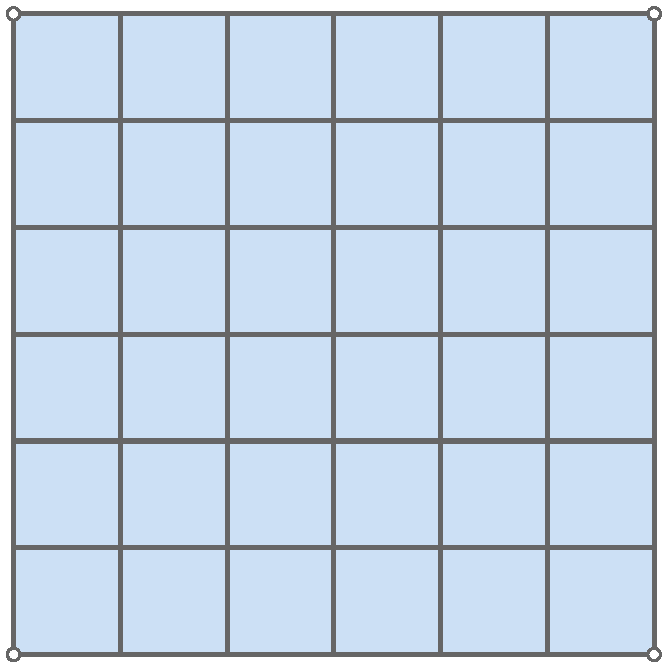
\includegraphics[width=0.2\textwidth]{planar_circles/schramm_image-new}}\hfill%
\raisebox{-0.5\height}{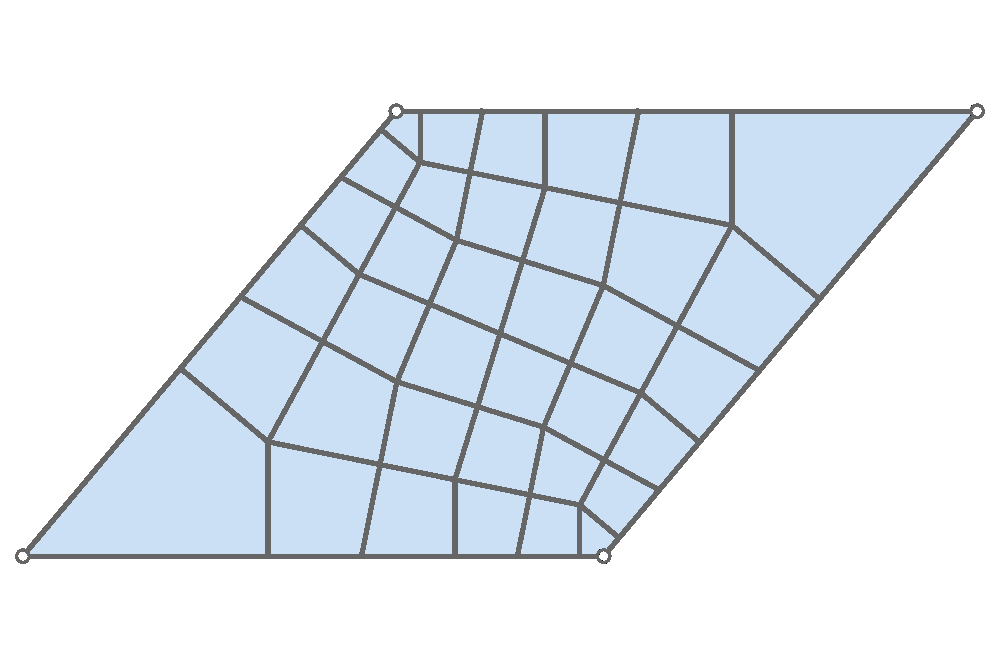
\includegraphics[width=0.4\textwidth]{planar_circles/schramm_quads-new}}\hspace{-0.05\textwidth}%
\raisebox{-0.5\height}{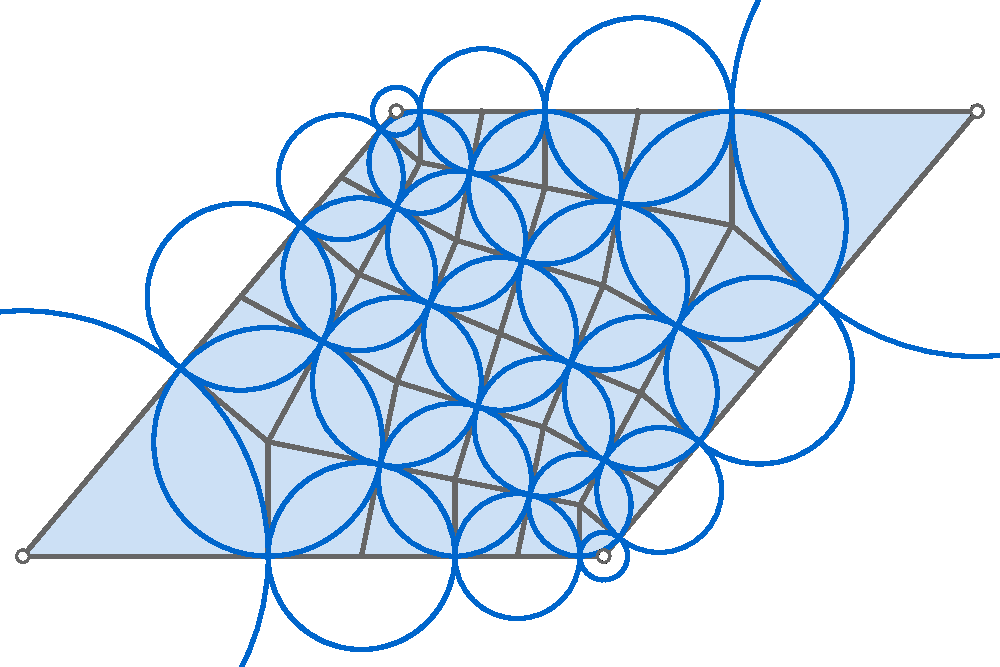
\includegraphics[width=0.4\textwidth]{planar_circles/schramm_circles-new}}\\
\scriptsize\tt data/planar\_circles/circular\_schramm02.xml\\
\raisebox{-0.46\height}{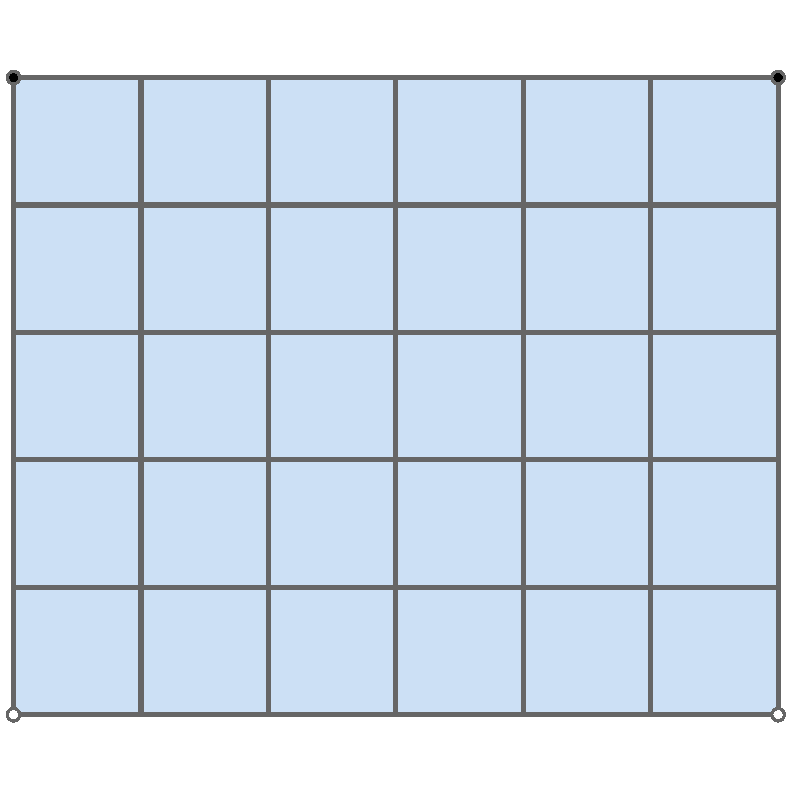
\includegraphics[width=0.2\textwidth]{planar_circles/non_schramm_image-new}}\hfill%
\raisebox{-0.5\height}{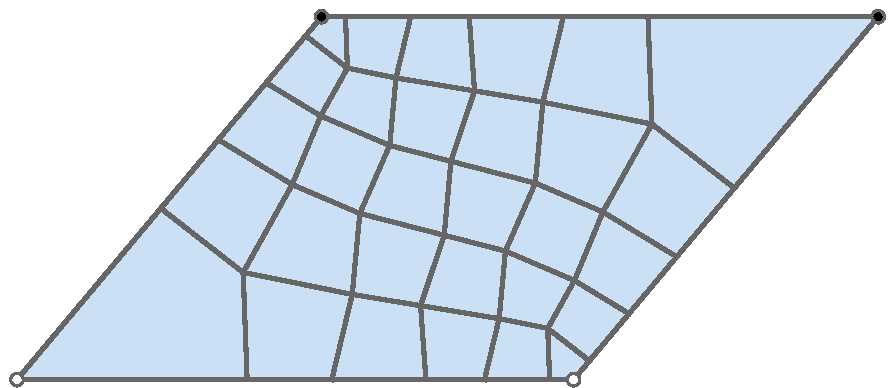
\includegraphics[width=0.4\textwidth]{planar_circles/non_schramm_quads-new}}\hspace{-0.05\textwidth}%
\raisebox{-0.5\height}{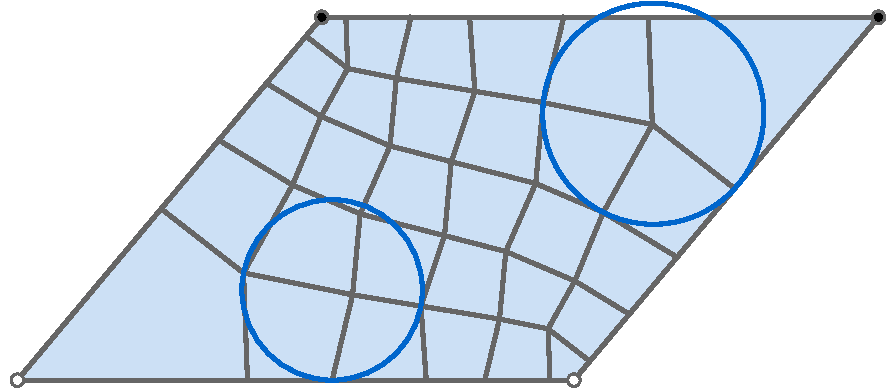
\includegraphics[width=0.4\textwidth]{planar_circles/non_schramm_circles-new}}\\
\scriptsize\tt data/planar\_circles/circular\_non\_schramm02.xml\\
\caption{
Mapping a rectangle to a parallelogram. Note the orthogonal circle
pattern in the top row and the wiggly vertical lines
in the bottom row. 
% All quadrilaterals in the image are cyclic quadrilaterals.
% Note, in addition to the circle pattern generated by the quadrilaterals the upper example yields an S-isothermic circle pattern whereas the lower one does not.
}
\label{fig:cyclic_parallelogram}
\end{figure}


On first sight, the $6\times 6$ example shown in the top row behaves
rather like one would expect from a conformal map. The horizontal and
vertical ``coordinate lines'' of the domain are mapped to polygonal
curves that look more or less like they could be discretizations of
reasonable smooth curves. In the $6\times 5$ example shown in the
bottom row, the images of the vertical lines zigzag noticeably.

A closer look at the $6\times 6$ example reveals a remarkable
phenomenon. Let us bicolor the vertices black and white so that
neighboring vertices have different colors, with the corners colored
white. Then, in the image quadrangulation, the edges incident with a
black vertex meet at right angles, and the edges incident with a white
vertex have the same length. One can therefore draw a circle around
each white vertex through the neighboring black vertices as shown in
Figure~\ref{fig:cyclic_parallelogram} (top right). At the black
vertices, these circles touch and intersect orthogonally. Such circle
patterns were studied by Schramm~\cite{S97} as discrete analogs of
conformal maps.

Given such a circle pattern with orthogonally intersecting circles,
the quadrangulation formed by drawing edges between circle centers and
intersection points consists of quadrilaterals that are right-angled
kites. Such kites have complex cross-ratio $-1$. Hence, the
quadrangulation coming from an orthogonal circle pattern is discretely
conformally equivalent (in our sense) to a combinatorially equivalent
quadrangulation consisting of squares. 

The conformal map shown in the top row of
Figure~\ref{fig:cyclic_parallelogram} ``finds'' the orthogonal circle
pattern because that circle pattern exists and the conformal map is
unique (by Theorem~\ref{thm:uniqueness}). For the $6\times 5$ example shown
in the bottom row, a corresponding orthogonal circle pattern does not
exist. No matter which coloring is chosen, there are two black
vertices at which the total angle changes (from $90^{\circ}$ to
$50^{\circ}$ and $130^{\circ}$, respectively). The neighbors of a
vertex do not lie on a circle. Figure~\ref{fig:cyclic_parallelogram}
(bottom right) shows two circles drawn through three out of four neighbors.

% Note that if a Schramm-circle-pattern \cite{S97} exist for the given combinatorics and boundary data of the polyhedral surface than the minimizer realizes this pattern since its solution is the unique circle pattern with the given boundary conditions.
% If it does not exist we get a cyclic solution and no circle pattern, see Figure~\ref{fig:cyclic_parallelogram} top-row versus bottom-row.

If we map an $m\times n$ square grid to a parallelogram like in
Figure~\ref{fig:cyclic_parallelogram}, an orthogonal circle pattern
will appear if $m$ an $n$ are even. No such pattern will appear if one
of the numbers is even and the other is odd. What happens if both $m$
and $n$ are odd? In this case, the conformal map does not exist. The
corners with increasing angle and the corners with decreasing angle
would have different colors. This violates the necessary condition
expressed in the following theorem.

\begin{theorem}[Necessary condition for the existence of a conformal map]
  Let $\Sigma$ be an abstract quadrangulation of the closed disk, and
  let 
  \begin{equation*}
    z,\tilde z: V_{\Sigma}\rightarrow\C
  \end{equation*}
  determine two discretely conformally equivalent immersions of\/
  $\Sigma$ into the complex plane. Denote their angle sums at boundary
  vertices $v\in V_{\Sigma}$ by\/ $\Theta_{v}$ and\/
  $\tilde\Theta_{v}$, respectively. Since the $1$-skeleton of\/~$\Sigma$ is
  bipartite, we may assume the vertices are colored black and
  white. Let $V^{\partial}_{b}$ and $V^{\partial}_{w}$ denote the sets
  of black and white boundary vertices of\/~$\Sigma$. Then
  \begin{align}
    \label{eq:boundary_black}
    \sum_{v\in V^{\partial}_b}(\tilde\Theta_v - \Theta_v)
    &\equiv 0 \pmod{2\pi},\\
    \label{eq:boundary_white}
    \sum_{v\in V^{\partial}_w}(\tilde\Theta_v - \Theta_v)
    &\equiv 0 \pmod{2\pi}.
  \end{align}
  (Since $\sum_{V^{\partial}_b \cup
    V^{\partial}_w}(\tilde\Theta_{v}-\Theta_{v})=0$,
  equations~\eqref{eq:boundary_white} and~\eqref{eq:boundary_black}
  are equivalent.)
\end{theorem}

\begin{proof}
  Since $z$ and $\tilde z$ are two solutions of the cross-ratio system
  on $\Sigma$ with the same cross-ratios (see
  Section~\ref{sec:quads}), there exists by
  Proposition~\ref{prop:complex_factors} a function
  $w:V_{\Sigma}\rightarrow\C$ such that~\eqref{eq:complex_factors}
  holds for all edges $\mathit{ij}\in E_{\Sigma}$. Now suppose
  $v_{0},\ldots,v_{2n-1}\in V_{\Sigma}$ are the boundary vertices in
  cyclic order (with indices taken modulo $2n$). Then
  \begin{equation*}
    e^{i(\tilde\Theta_{v_{k}} - \Theta_{v_{k}})}=
    \frac{(\tilde z_{v_{k+1}}-\tilde z_{v_{k}})(z_{v_{k-1}}-z_{v_{k}})}%
    {(\tilde z_{v_{k-1}}-\tilde z_{v_{k}})(z_{v_{k+1}}-z_{v_{k}})}
    =\frac{w_{v_{k+1}}}{w_{v_{k-1}}},
  \end{equation*}
  so
  \begin{equation*}
    \prod_{k=0}^{n-1}e^{i(\tilde\Theta_{v_{2k}} - \Theta_{v_{2k}})}=
    \prod_{k=0}^{n-1}e^{i(\tilde\Theta_{v_{2k+1}} -
      \Theta_{v_{2k+1}})}=
    1.
  \end{equation*}
  Equations~\eqref{eq:boundary_black} and~\eqref{eq:boundary_white}
  follow.
\end{proof}

% In the examples of Figure~\ref{fig:cyclic_parallelogram} this condition is met. 
% In the top example all corners have the same color, thus all curvature changes add up and cancel.
% In the second example the two bottom corners have a different color than the two top corners.
% As the result is a parallelogram again the change of angles cancels out.
% On the contrary, a square made from $7$ squares in each direction does not meet the condition with the given boundary angles.
% Here opposite corners have the same color.
% The change of curvature has the same sign for opposite corners, hence the conditions are not true.
% Experiments show that we cannot solve the problem in such a case.

\subsection{Riemann maps with cyclic quadrilaterals}
\label{sec:riemann_map}

Consider the following discrete version of the Riemann mapping
problem: Map a cyclic polyhedral surface that is topologically a
closed disk discretely conformally to a planar polygonal region with
boundary vertices on a circle. An example is shown in
Figure~\ref{fig:circular_riemann}, top row. 
\begin{figure}
  \newlength{\savetextwidth}\setlength{\savetextwidth}{\textwidth}
  \begin{picture}(0,0)
    \includegraphics[width=0.5\savetextwidth]{planar_circles/riemann_shape_image.pdf}%
  \end{picture}
  \setlength{\unitlength}{\savetextwidth}
  \begin{picture}(0.5,0.458056)
    \put(0.3,0.102){$k$}
  \end{picture}
  \includegraphics[width=0.5\textwidth]{planar_circles/riemann_shape_domain.pdf}\\
  \hspace*{0.4\textwidth}%
  \Large%
  $\downarrow$%
  \hspace{0.24\textwidth}%
  \rotatebox{-20}{$\uparrow$}\\
  \hspace*{\fill}%
  \includegraphics[height=6.5cm]{planar_circles/riemann_shape_halfplane.pdf}%
  \hspace*{\fill}
  \begin{center}
  \setstretch{0.0}{\scriptsize\tt data/planar\_circles/riemann\_shape.xml}
  \end{center}
  \caption{Riemann mapping with cyclic quadrilaterals.
Corners with valence two in the original domain are modeled as triangles, upper left.
We first map to the upper half-plane.
Quadrilaterals adjacent to the point at infinity are removed.
Points opposite to the point at infinity have a prescribed boundary angle of $\pi$.
The four vertices in between have a fixed $u=0$.
Quadrilaterals adjacent to the point at infinity are cyclic after the M{\"o}bius transformation to the disk, bottom.  
  }
  \label{fig:circular_riemann}
\end{figure}
This type of problem can often be reduced to
Problem~\ref{prob:factors_and_angles}. Then, by the variational
principle, if a solution exists, it can be found by minimizing a
convex function. For triangulations, the reduction of the discrete
Riemann mapping problem to Problem~\ref{prob:factors_and_angles} is
explained by Bobenko {\it et al.}\ \cite[Section 3.3]{BPS2015:dconf}. Here, we consider the
case of quadrangulations. (The arguments can be extended to even
polygons with more than four sides. We restrict our attention to
quadrilaterals because the combinatorial restrictions discussed in the
following paragraph become even more involved yet not more interesting for 
surfaces with hexagons, octagons, etc.)

The basic idea is the same as for triangulations: First, map the
polyhedral surface to the half plane with one boundary vertex at
infinity. Then apply a M{\"o}bius transformation. This leads to a
combinatorial restriction: No face may have more than one edge on the
boundary. (The face would degenerate when the boundary is mapped to a
straight line.) For triangulations, this means that no triangle may be
connected to the surface by only one edge. If this condition is
violated, cutting off such ``ears'' often leads to an admissible
triangulation. For quadrangulations, this fix does not work in typical
situations. Instead, if a quadrilateral contains two consecutive edges
on the boundary, cut off a triangle. The resulting polyhedral surface
will consist mostly of quadrilaterals with some triangles on the
boundary, as in the example shown in Figure~\ref{fig:circular_riemann}.

\begin{figure}
  \centering
  \includegraphics[width=0.5\textwidth]{planar_circles/riemann_shape_circles.pdf}\\
  \setstretch{0.0}{\scriptsize\tt data/planar\_circles/riemann\_shape.xml}
  \caption{Here we show the face circumcircles of the solution to the
    Riemann mapping problem of Figure~\ref{fig:circular_riemann}. It
    looks conspicuously like an orthogonal circle pattern. But the
    face circumcircles intersect only approximately but not exactly at
    right angles.}
  \label{fig:riemann_circles}
\end{figure}

% \begin{figure}
% \centering
% \resizebox{\textwidth}{!}{
% \includegraphics[height=5cm]{planar_circles/riemann_shape_image.pdf}
% \quad
% \raisebox{0.75cm}{
% \includegraphics[height=3.5cm]{planar_circles/riemann_shape_closeup.pdf}
% }
% }
% \resizebox{0.9\textwidth}{!}{
% \includegraphics[height=5cm]{planar_circles/riemann_shape_halfplane.pdf}
% }
% \resizebox{\textwidth}{!}{
% \includegraphics[height=5cm]{planar_circles/riemann_shape_domain.pdf}
% \includegraphics[height=5cm]{planar_circles/riemann_shape_circles.pdf}
% }
% \caption{
% Riemann-map with cyclic quadrilaterals.
% Corners with valence two in the original domain are modeled as triangles, upper left.
% We first map to the upper half-plane.
% Quadrilaterals adjacent to the point at infinity are removed.
% Points opposite to the point at infinity have a prescribed boundary angle of $\pi$.
% The four vertices in between have a fixed $u=0$.
% By that quadrilaterals adjacent to the point at infinity are cyclic after the Moebius transformation to the disk, bottom.
% }
% \label{fig:circular_riemann}
% \end{figure}

Suppose $(\Sigma,\ell)_{\euc}$ is a euclidean cyclic polyhedral
surface that is homeomorphic to the closed disk and consists mostly of
quadrilaterals. (For the following construction we really only need a
boundary vertex that is incident with quadrilateral faces.) To map it
to a polygonal region inscribed in a circle, proceed as follows (see
Figure~\ref{fig:circular_riemann}):

% We show how to calculate discrete Riemann maps for cyclic quadrilateral domains, i.e., a discrete analog of conformal maps from a simply connected planar region to the unit disk. 
% In particular this yields a method for the generation of circle pattern Riemann maps, see Figure~\ref{fig:circular_riemann}.
% The procedure is in many aspects analogous to the previously described method for triangulations \cite{BPS2015:dconf}.
% Let $\Sigma$ be a cyclic planar domain that consists solely of quadrilaterals and $\ell$ be a discrete metric on $\Sigma$. 
% Proceed as follows:

\begin{compactenum}[(1)]
\item Choose a vertex $k$ on the boundary of $\Sigma$ such that all
  incident faces are quadrilaterals.
\item Apply a discrete conformal change of
  metric~\eqref{eq:tilde_ell_euc} such that all edges incident
  with~$k$ have the same length. One may choose $u=0$ for all
  vertices except the neighbors of~$k$. It does not matter if polygon
  inequalities are violated after this step.
\item Let $(\Sigma',\ell')_{\euc}$ be the cyclic polyhedral complex obtained by 
  removing vertex $k$ and all incident quadrilaterals.
\item Solve Problem~\ref{prob:factors_and_angles} for
  $(\Sigma',\ell')_{\euc}$ with prescribed total angles
  $\Theta_i=2\pi$ for interior vertices of $\Sigma'$, $\Theta_i=\pi$
  for boundary vertices of $\Sigma'$ that were not neighbors of $k$ in
  $\Sigma$, and fixed logarithmic scale factors $u_i=0$ for those that
  were neighbors of $k$. The result is a planar polyhedral surface as
  shown in Figure~\ref{fig:circular_riemann}, bottom. The boundary
  consists of one straight line segment containing all boundary edges
  of $\Sigma'$ that were also boundary edges of $\Sigma$, and two or
  more straight line segments, each consisting of two edges that were
  incident with a removed quadrilateral.
\item Apply a M{\"o}bius transformation (e.g., $z\mapsto 1/z$) to the
  vertices that maps the boundary vertices of $\Sigma$ to a circle and
  the other vertices to the inside of this circle. Reinsert $k$ at the image
  point of $\infty$ under this M{\"o}bius transformation. Each face
  ${\it ijmk} \in \Sigma$ incident with $k$ is cyclic because the three
  vertices $i$, $j$, and $m$ are contained in a line before
  transformation.
\item Optionally apply a 2-dimensional version of the M{\"o}bius
  normalization described in Section~\ref{sec:moebius_normalization}.
\end{compactenum} 

\begin{proposition}
  \label{prop:riemann_map}
  The result of this procedure is a planar cyclic polyhedral surface
  that is discretely conformally equivalent to $(\Sigma, \ell)_{\euc}$
  and has its boundary polygon inscribed in a circle.
\end{proposition}

\goodbreak
\begin{proof}
  That the boundary polygon is inscribed in a circle is obvious from
  the construction.  Using the M{\"o}bius invariance of discrete
  conformal equivalence (Proposition~\ref{prop:Moebius_inv}), it is
  not difficult to see that the surfaces without quadrilaterals
  incident with $k$ are discretely conformally equivalent. To show
  that the whole surfaces are equivalent, it suffices to show that
  corresponding quadrilaterals incident with $k$ have the same complex
  cross-ratio.

  After step (2), the length cross-ratio of a quadrilateral incident with
  $k$ is equal to the simple length ratio of the two edges that are
  not incident with $k$. 

  After step (4), the length cross-ratio of these edges is unchanged due
  to the fixed logarithmic scale factors $u=0$ on the neighbors of
  $k$. Also, these edges are now collinear because of the prescribed
  angle $\Theta=\pi$ between them.

  After applying the M{\"o}bius transformation in step (5), the image of
  the point at infinity and the other three vertices of our
  quadrilateral incident with $k$ form again a cyclic quadrilateral
  with the same complex cross-ratio as in the beginning.
\end{proof}

\section{Multiply connected domains}
\label{sec:multiply_connected}

\subsection{Circle domains}
\label{sec:circle_domains}

Koebe's generalization of the Riemann mapping theorem says that
multiply connected domains are conformally equivalent to domains
bounded by circles, and the uniformizing map to such a circle domain
is unique up to M{\"o}bius transformations. A method to construct
discrete Riemann maps is described by Bobenko {\it et al.}\ \cite[Section
3.3]{BPS2015:dconf} for triangulations and for mostly quadrilateral meshes in
the previous Section~\ref{sec:riemann_map}. Having generalized the
notion of discrete conformal equivalence from triangulations to cyclic
polyhedral surfaces, it is straightforward to adapt this method to
construct discrete maps to circle domains: 

\begin{compactenum}[(1)]
\item Fill holes by gluing faces to all but one boundary component,
  so that the resulting surface is homeomorphic to a disk.
\item Construct the discrete Riemann map.
\item Remove the faces that were added in step (1). 
\end{compactenum}

Figure~\ref{fig:euclidean_circle_domain} shows an example.
\begin{figure}
\centering
\includegraphics[width=0.3333\textwidth]{circle_domain_euclidean/three_holes_image.pdf}%
\includegraphics[width=0.3333\textwidth]{circle_domain_euclidean/three_holes_domain.pdf}%
\includegraphics[width=0.3333\textwidth]{circle_domain_euclidean/three_holes_map.pdf}\\
\setstretch{0.8}{\scriptsize\tt data/circle\_domain\_euclidean/three\_holes.xml}
\caption{
Discrete conformal map of a multiply-connected domain (left) to a
circle domain (middle). The images of vertical and horizontal ``parameter
lines'' are shown on the right.
}
\label{fig:euclidean_circle_domain}
\end{figure}

% We call a cyclic planar domain a circle domain if the vertices of each boundary component are inscribed in a circle.
% In this section we present discrete conformal maps from planar domains to circle domains, see Figure~\ref{fig:euclidean_circle_domain}.
% There is an analogous theorem for surfaces with higher genus, see Section~\ref{sec:hyperbolic_circle_domain} and Figure~\ref{fig:hyperbolic_circle_domain}.
% In the smooth setting the corresponding theorem has been conjectured by Koebe. 
% Every domain in $\C$ is conformally equivalent to a domain bounded by circles.
% The process to calculate a discrete map from a discrete planar cyclic domain to a discrete circle domain is as follows.
% Suppose there is a unique exterior boundary component. Fill all interior boundary components by attaching faces. 
% Triangulate the new faces to produce a set of new edges $E_2$. 
% Let $\lambda_{\it ij}$ with $\it ij\in E_2$ be free variables of the mapping problem.
% Map the domain to a circle as described in Section~\ref{sec:riemann_map} by solving Problem~\ref{prob:factors_and_angles} with these extra variables.
% Remove extra edges $\it ij\in E_2$.
% The boundary vertices of the result are inscribed in circles, see Figure~\ref{fig:euclidean_circle_domain}.

\subsection{Special slit domains}

Any multiply connected domain can be mapped to the complex plain with
parallel slits~\cite{nehari1952conformal}. In principle, it is
possible to construct discrete conformal maps that map holes to slits
by solving Problem~\ref{prob:total_angles}. On each boundary component
that should be mapped to a slit, set the desired total angle
$\Theta=2\pi$ for the two vertices that should be mapped to the
endpoints of the slit, and set $\Theta=\pi$ for all other vertices on
that boundary component. However, this will not work in general. While
the resulting surface will be flat, the developing map to the plane
will in general have translational monodromy for a cycle around the
hole. The surface will only close up in the plane if the vertices that
should be mapped to the endpoints of the slit are chosen exactly
right. (This will in general require modifying the original mesh.)

Sometimes, the symmetry of the problem determines the right positions
of the end-vertices, so that discrete conformal maps to slit surfaces
can be computed. The first two rows of Figure~\ref{fig:fluid_flows}
show examples. The bottom row visualizes a discrete conformal map
where circular holes are mapped to slits. Here, we use the following
trick: We start with the slit surface and map it to a surface with
circular holes as described in Section~\ref{sec:circle_domains}.
\begin{figure}
	\centering
	\resizebox{\textwidth}{!}{
	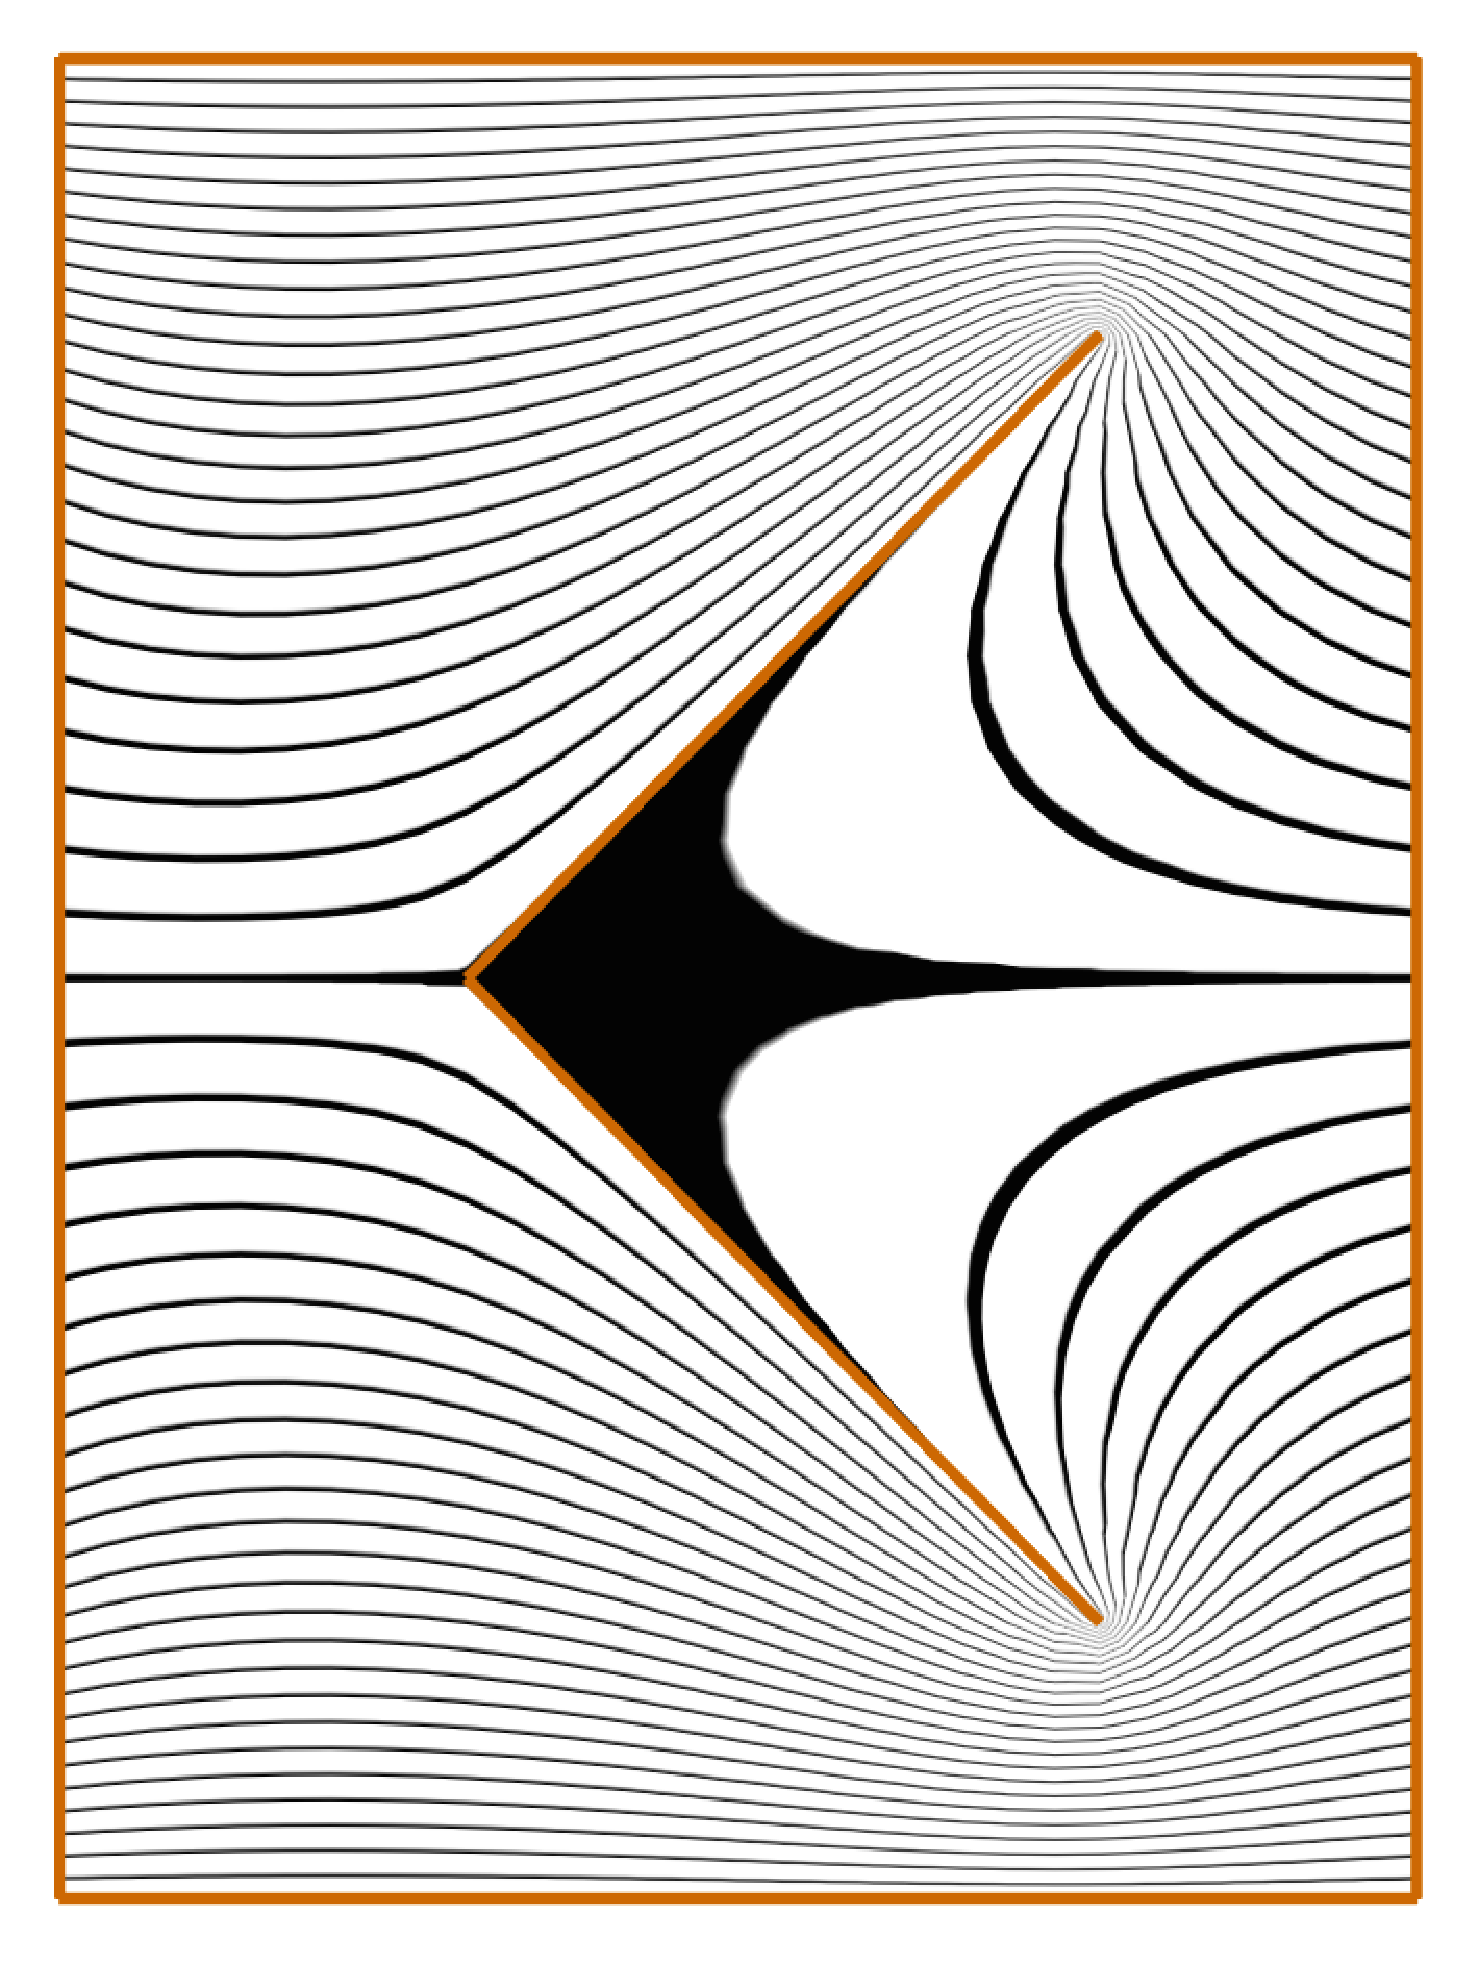
\includegraphics[height=5cm]{planar_streams/arrow_cylinder.pdf}
	\hskip 0.01\textwidth
	\includegraphics[height=5cm]{planar_streams/arrow_cylinder_image.pdf}\hfill
	\hskip 0.01\textwidth
	\includegraphics[height=5cm]{planar_streams/arrow_cylinder_domain.pdf}
	}
	\setstretch{0.0}{\scriptsize\tt data/planar\_streams/arrow\_cylinder\_planar.xml}
	\resizebox{\textwidth}{!}{
	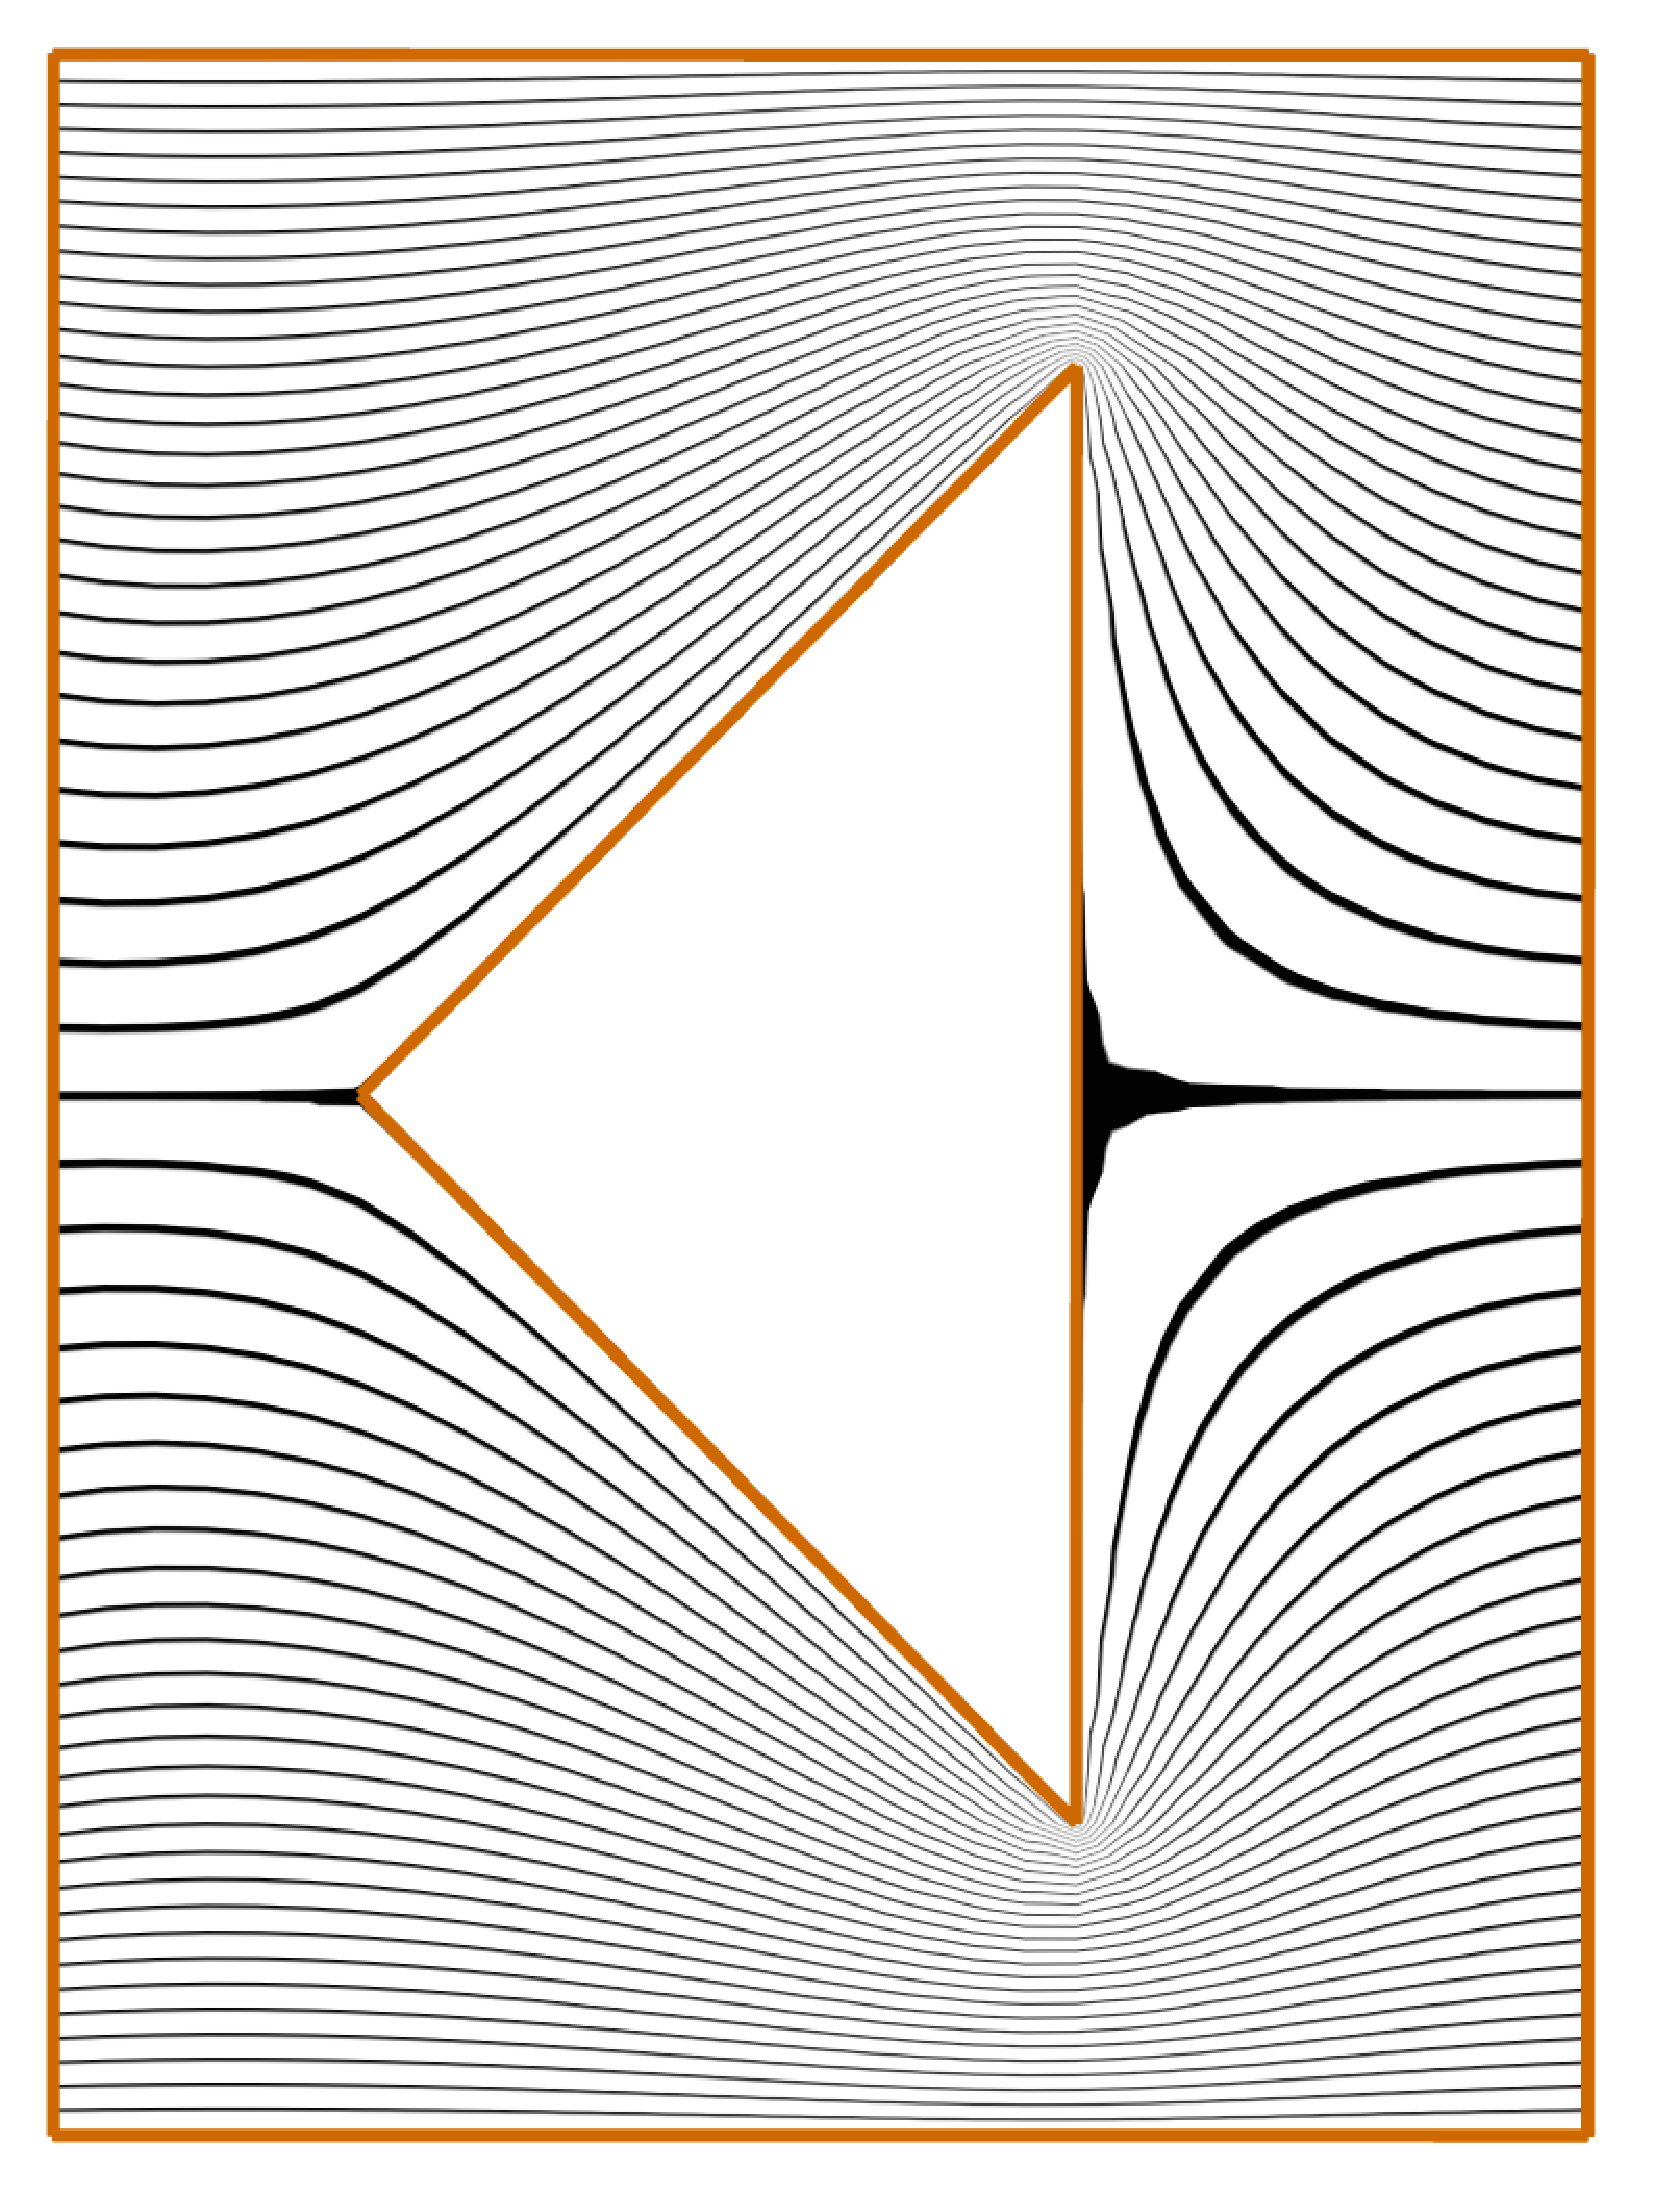
\includegraphics[height=5cm]{planar_streams/triangle_cylinder.pdf}
	\hskip 0.01\textwidth
	\includegraphics[height=5cm]{planar_streams/triangle_cylinder_image.pdf}\hfill
	\hskip 0.01\textwidth
	\includegraphics[height=5cm]{planar_streams/triangle_cylinder_domain.pdf}
	}
	\setstretch{0.0}{\scriptsize\tt data/planar\_streams/triangle\_cylinder\_planar.xml}
	\resizebox{\textwidth}{!}{
	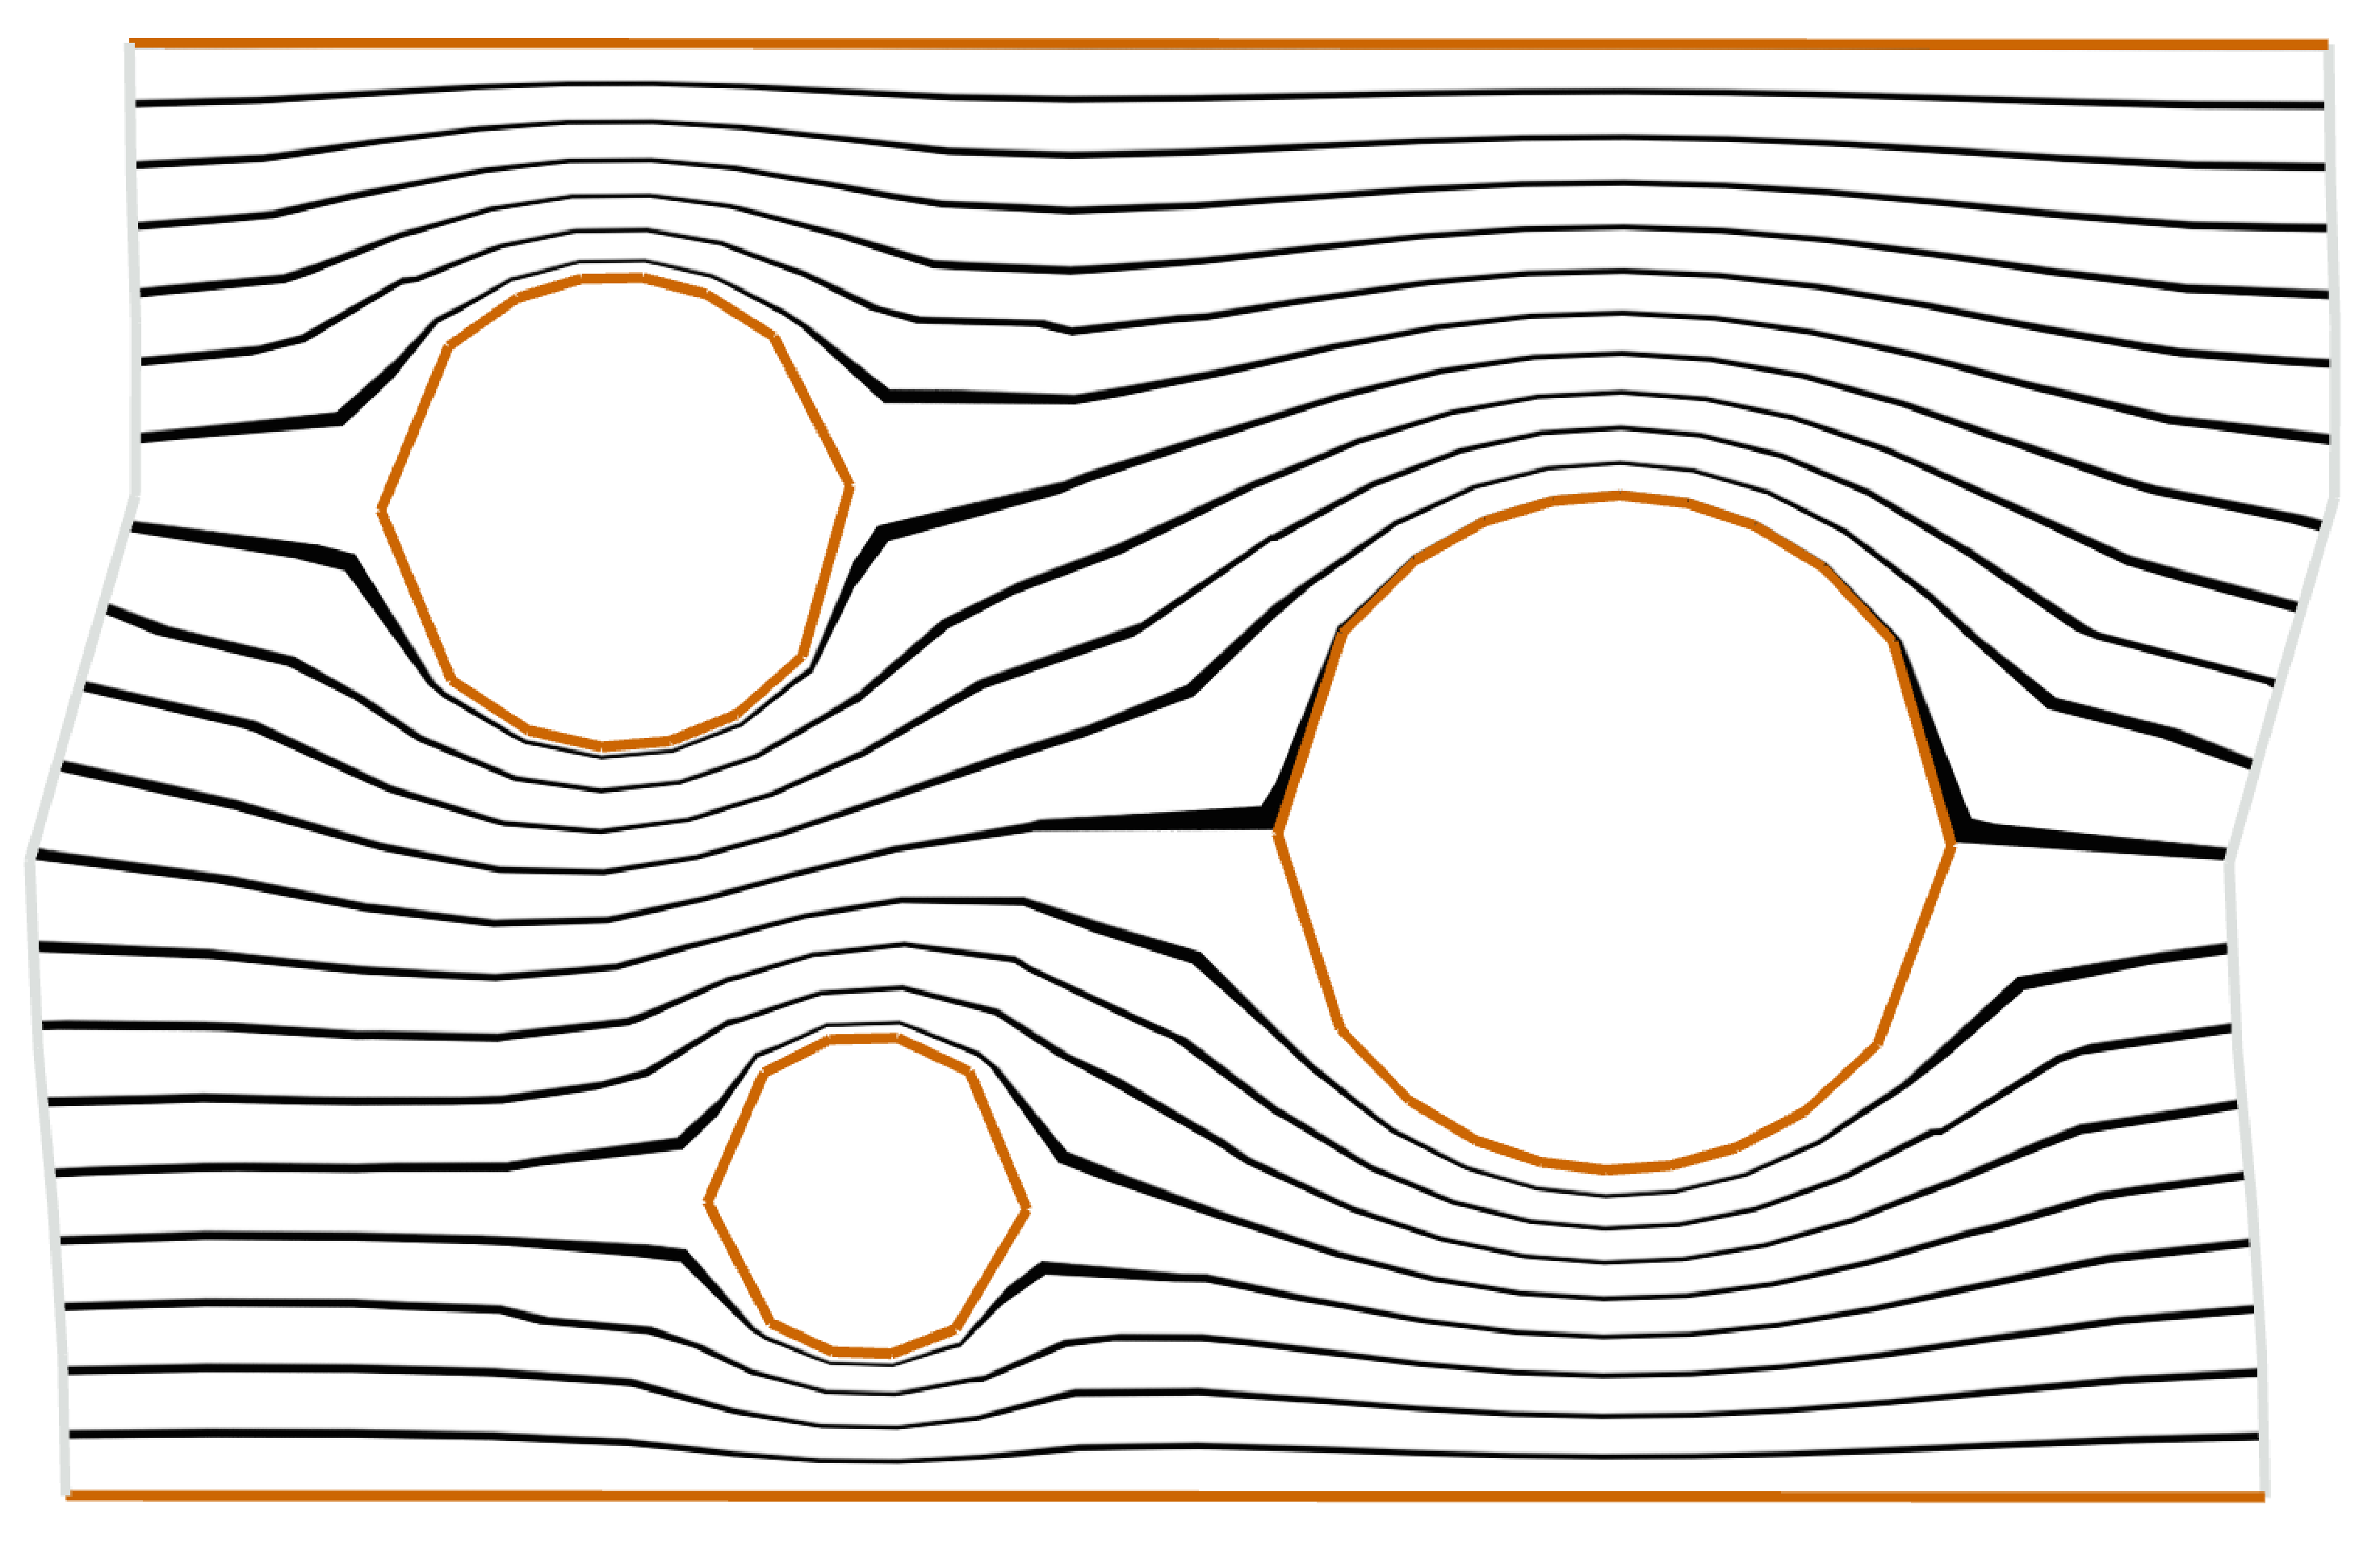
\includegraphics[height=5cm]{planar_streams/circular_stream_03_lines.pdf}
	\includegraphics[height=5cm]{planar_streams/circular_stream_03_mesh.pdf}
	}
	\setstretch{0.0}{\scriptsize\tt data/planar\_streams/circular\_stream\_03.xml}
        \caption{Mapping surfaces with holes to slit surfaces. In all
          images, the left and right parts of the boundary are
          identified by a horizontal translation. Preimages of
          horizontal lines visualize the flow of an incompressible
          inviscid fluid around the hole in a channel with periodic
          boundary conditions. Top row: A
          cylinder with a triangular hole is mapped to a cylinder with
          a slit. One vertex of the triangle and the midpoint of the
          opposite side are mapped to the endpoints of the
          slit. Middle row: An arrow shaped slit is mapped to a
          straight slit. The two vertices at the arrow's tip, on either
          side of the slit, are mapped to the endpoints of the
          straight slit. Bottom row: Three circular boundary
          components are mapped to horizontal slits. (The slit surface
          is not shown.)}
\label{fig:fluid_flows}
\end{figure}

% In this section we show how to conformally map multiply connected planar domains.
% Our examples are inspired by planar potential flows with periodic boundary conditions, see Figure~\ref{fig:fluid_flows}.
% The basic idea is to map a given domain with boundary components to periodic region with parallel slits.
% We do not solve the general problem of discretely mapping an arbitrary region to a domain with parallel slits here but provide a few examples where we could obtain nice results using discrete conformal mappings as defined above.

% In general the main challenge for the computation of such a map is to find the points on the boundary components that map to the ends of the slits. As these points may even not be located at vertices of the underlying mesh in general this involves a mesh refinement procedure. To solve the problem for the general case one would also have to solve an optimization problem to find the location of the points such that the slits become parallel and are oriented in a prescribed direction.

% In the first two examples we can derive the pre-images of the slit ends by symmetry. 
% We take a rectangle with two identified sides, i.e. a part of a topological cylinder and place a symmetric cut in the shape of an arrow, see Figure~\ref{fig:fluid_flows} upper-left. 
% By symmetry the vertices to the left and to the right of the arrow tip get mapped to the ends of the slits. 
% This implies that we want to calculate a symmetric flow with respect to the configuration.
% The boundary conditions are trivial. 
% All $\theta_i$ at the boundary are equal to $\pi$ except for the vertices at the tip of the arrow where $\theta$ is equal to $2\pi$.
% In the second example we cut a symmetric triangle to form a boundary component. The pre-images of the slit ends are the left corner of the triangle and the mid-point of the right side, see Figure~\ref{fig:fluid_flows} middle row.

% The third example is different from the other two as we inverse the direction of calculation. 
% The goal is to create a map from a domain with round holes to a region with parallel slits, see Figure~\ref{fig:fluid_flows} bottom row. 
% As we do not want to solve the global optimization problem for the location of the pre-images of slit ends we use a simple trick.
% We start with a cylinder with parallel slits.
% We add additional edges to triangulate the slits with the condition that none of the edges has zero length.
% Remember that the functional is linearly extended to triangulations with angles greater or equal than $\pi$.
% We treat the additional edges as auxiliary edges in a circular polygon, i.e., the corresponding $\lambda$s in the functional are variables of the optimization. 
% Thus adjacent triangles form a circular polygon in the resulting image.

\section{Uniformization of spheres}
\label{sec:spheres}

This section is concerned with discrete conformal maps of polyhedral
surfaces of genus~$0$ onto the round sphere. For triangulations, this
is described by Bobenko {\it et al.}\ \cite[Section 3.2]{BPS2015:dconf}. In
Section~\ref{sec:spheres_euclidean}, we adapt this method to
quadrangulations. This is similar to the discrete Riemann mapping with
quadrilaterals described in
Section~\ref{sec:riemann_map}. Effectively, this method reduces the
problem to minimizing the convex euclidean functional $E^{\euc}$. The
spherical version of the variational principle
(Theorem~\ref{thm:variational}) involves the non-convex
function~$E^{\sph}$. It is not as practical for calculations, because
one has to find a saddle point instead of a minimum. Nevertheless, the
spherical functional can often be used to calculate maps to the
sphere. This is explained in Section~\ref{sec:spherical_computation}.

\subsection{Uniformizing quadrangulations of the sphere}
\label{sec:spheres_euclidean}

\begin{figure}
\centering%
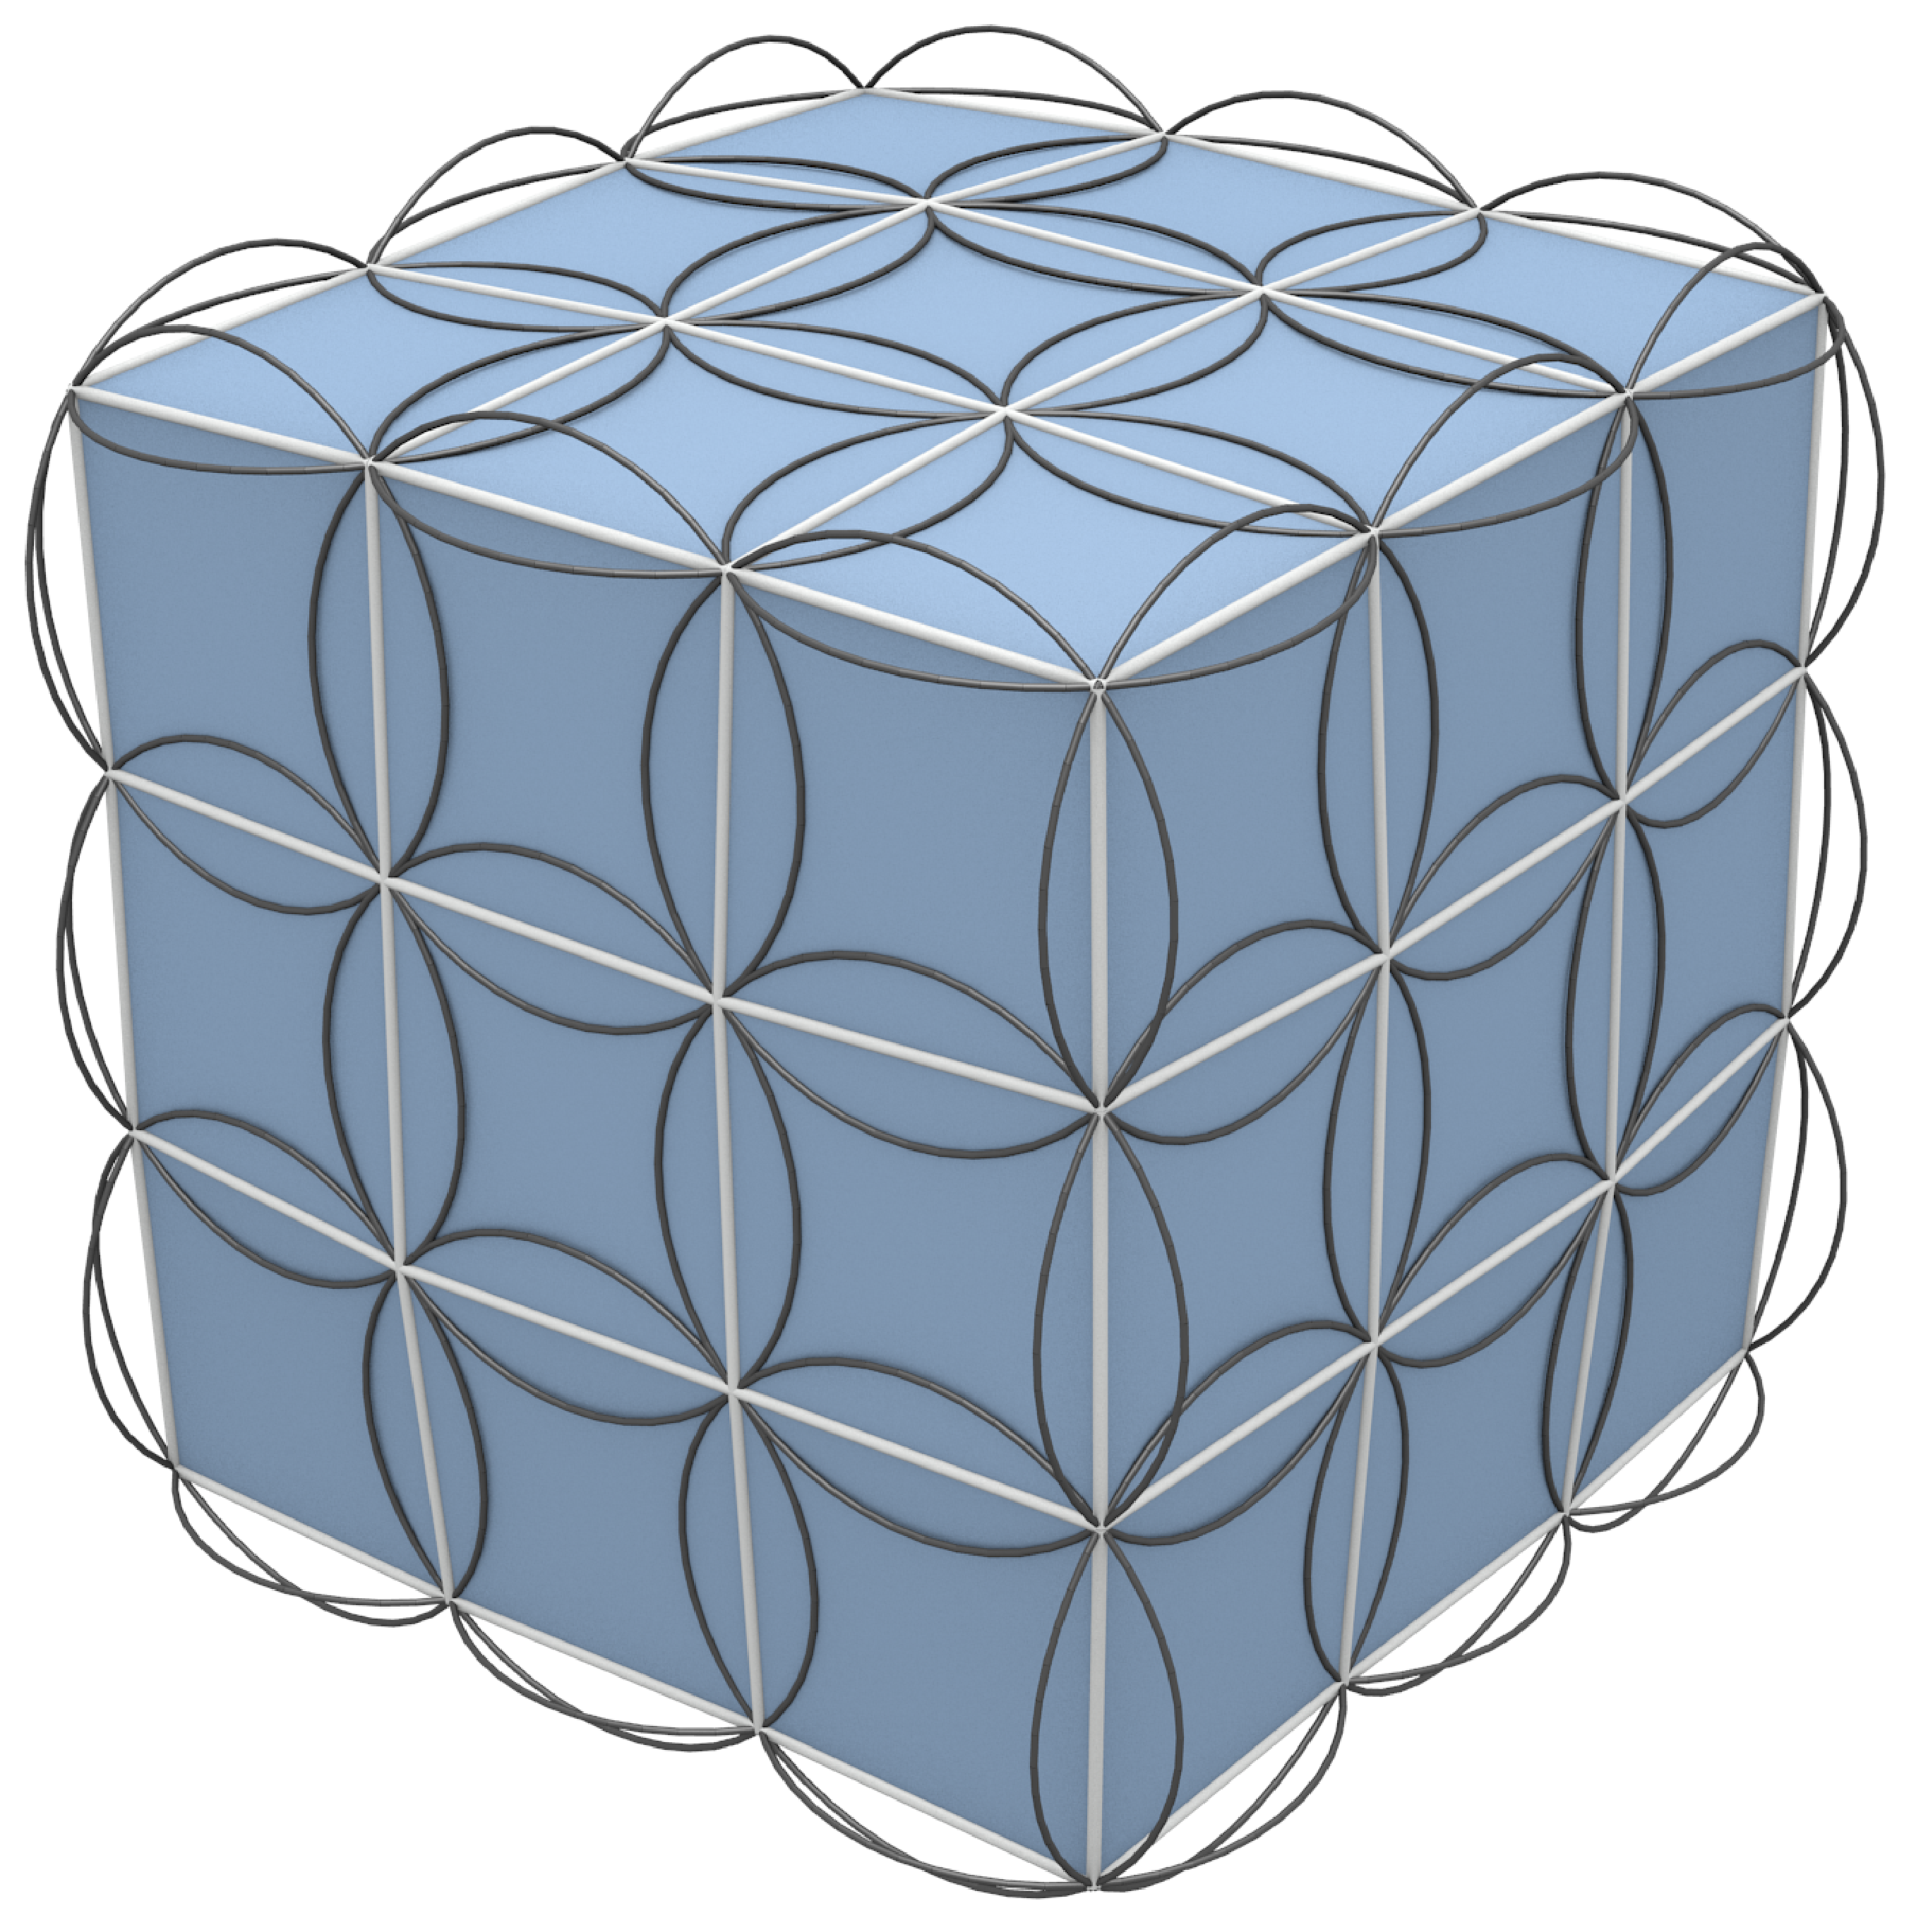
\includegraphics[width=0.4\textwidth]{spherical_cyclic/cube_cyclic_domain.pdf}%
\hspace{0.1\textwidth}%
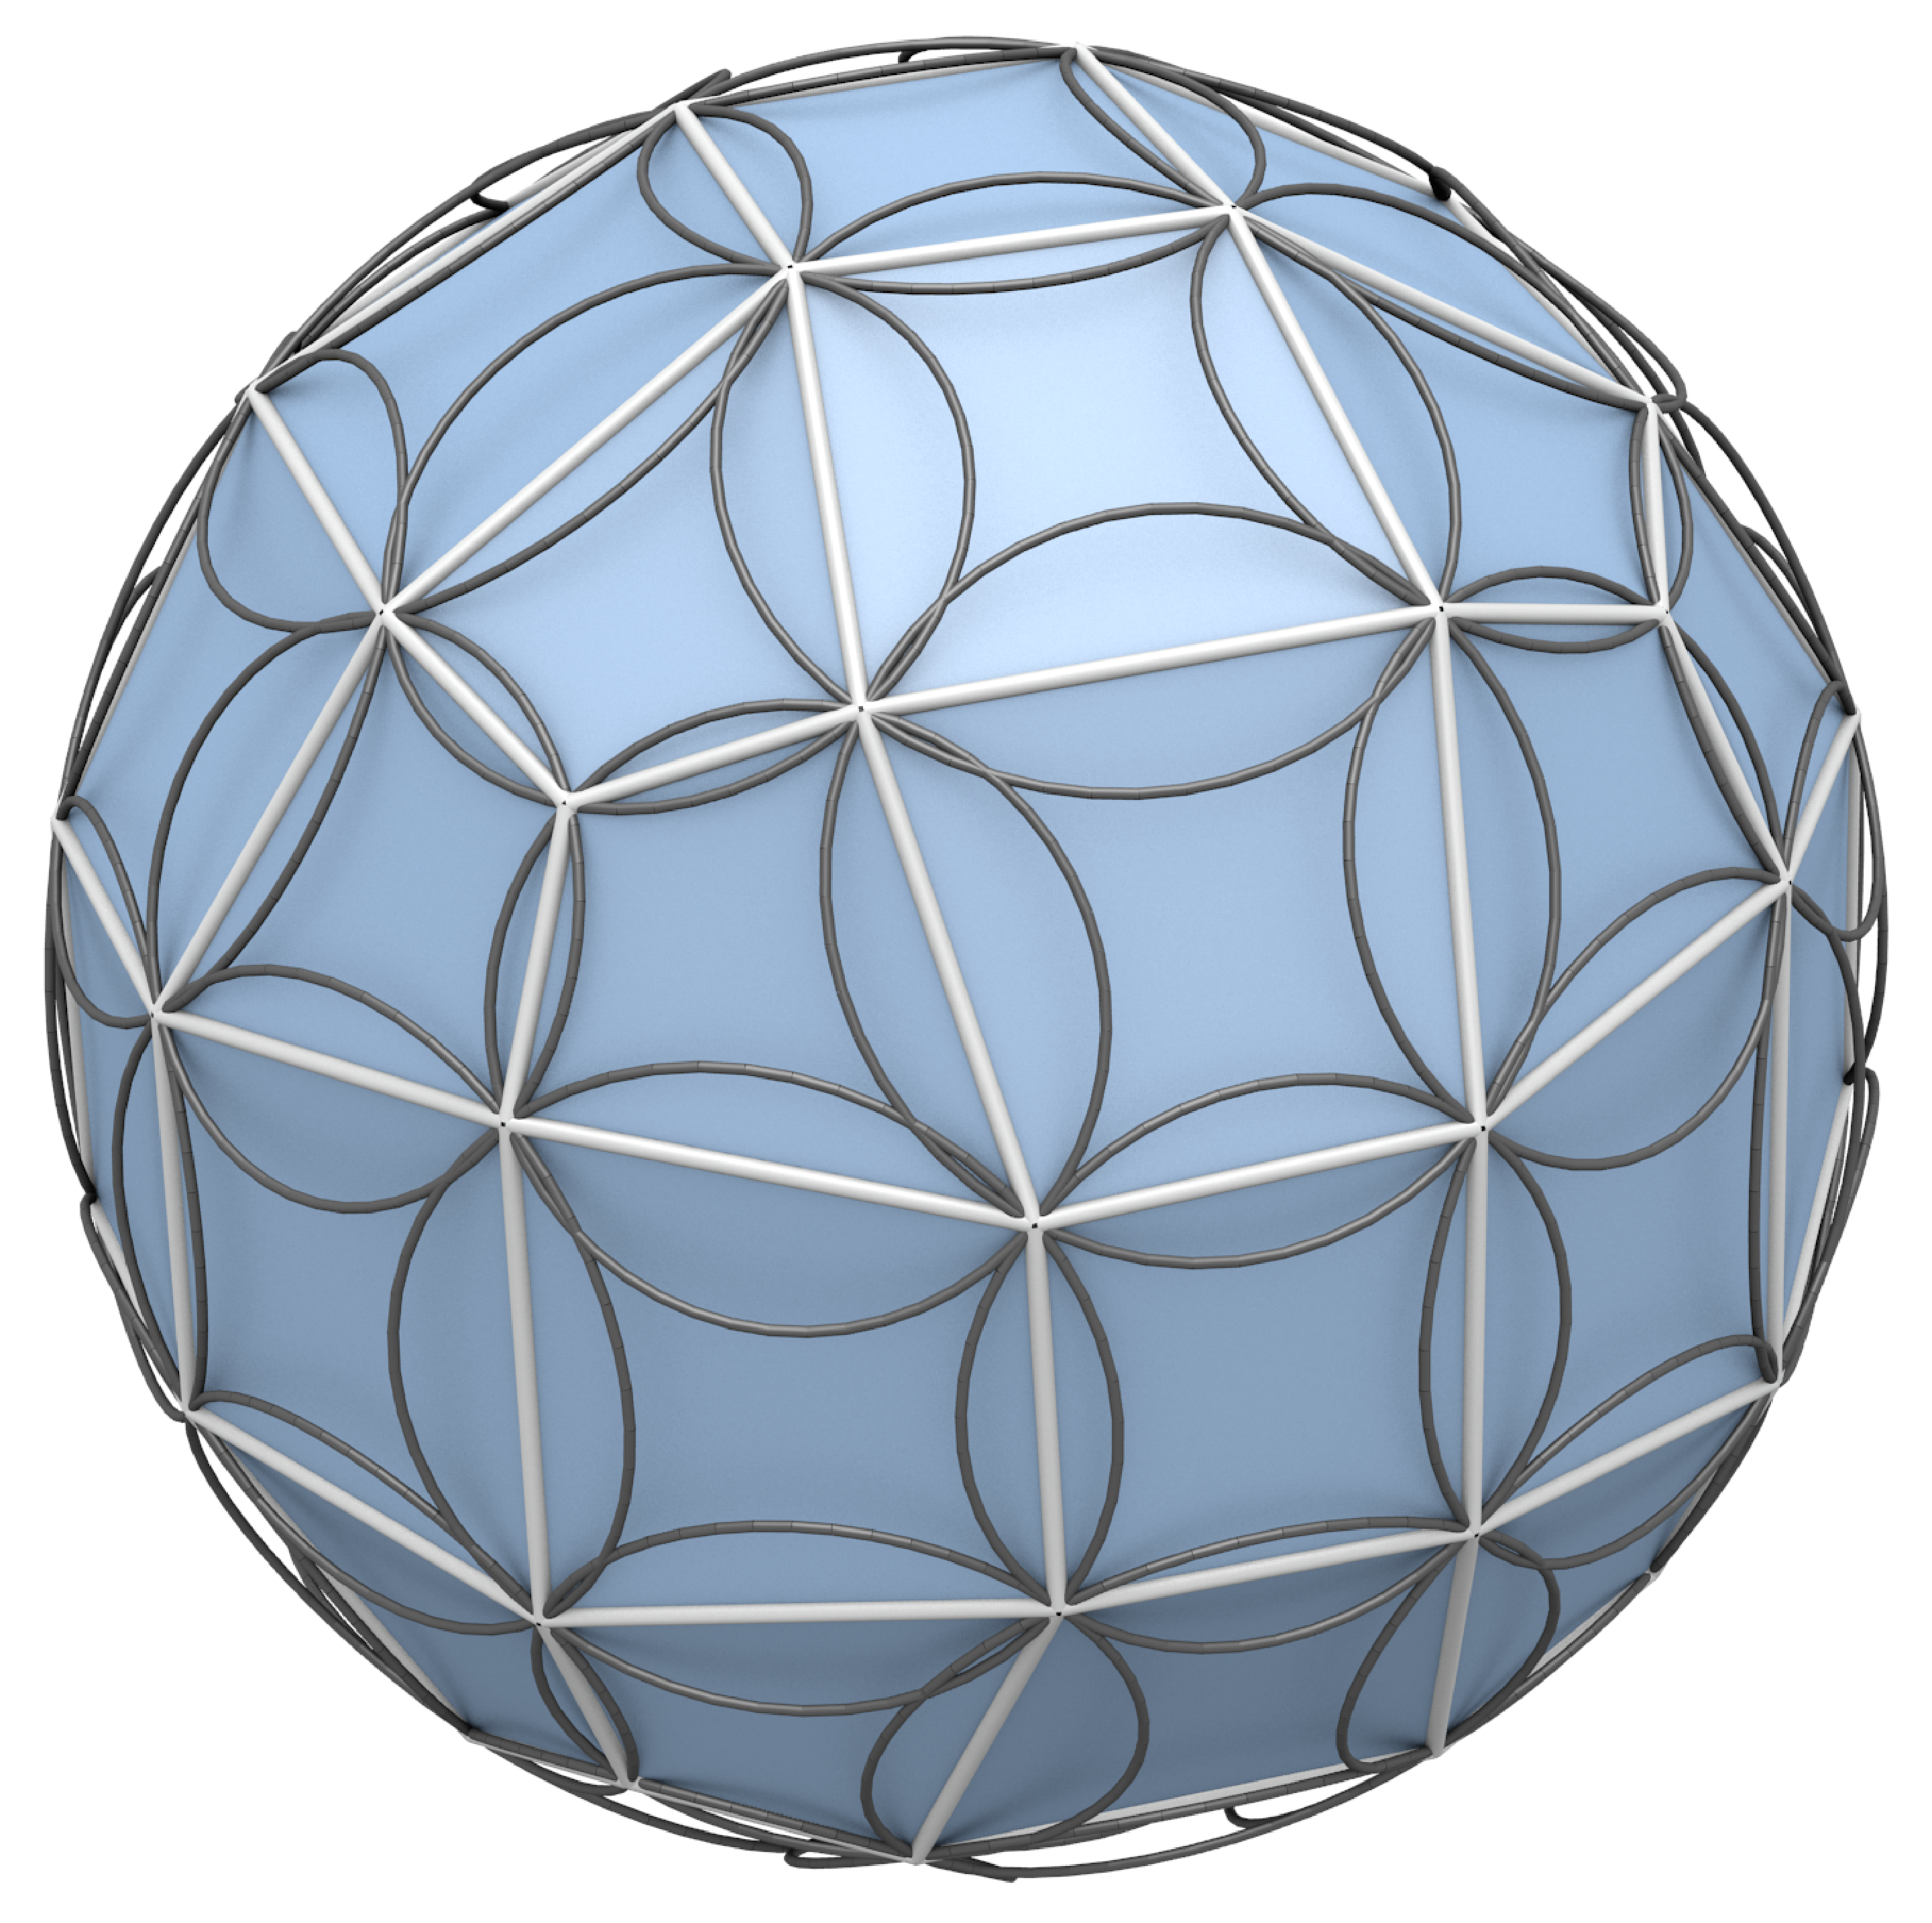
\includegraphics[width=0.4\textwidth]{spherical_cyclic/cube_cyclic_image.pdf}\\
\setstretch{0.0}{\scriptsize\tt data/spherical\_cyclic/spherical\_circular.xml}
\caption{Discrete conformal map from the cube to the sphere,
  calculated with the method described in
  Section~\ref{sec:spheres_euclidean}. We apply M{\"o}bius
  normalization (Section~\ref{sec:moebius_normalization}) to the
  polyhedral surface with vertices on the sphere to achieve rotational
  symmetry.}
\label{fig:spherical_circular}
\end{figure}

Suppose $(\Sigma,\ell)_{\euc}$ is a cyclic polyhedral surface with
quadrilateral faces that is homeomorphic to the sphere.
\begin{compactenum}[(1)]
\item Choose a vertex $k\in V_{\Sigma}$.
\item Apply a discrete conformal change of
  metric~\eqref{eq:tilde_ell_euc} such that all edges incident
  with~$k$ have the same length. One may choose $u=0$ for all
  vertices except the neighbors of~$k$. It does not matter if polygon
  inequalities are violated after this step. 
\item Let $(\Sigma',\ell')_{\euc}$ be the complex obtained by removing
  vertex $k$ and all incident quadrilaterals.
\item Solve Problem~\ref{prob:factors_and_angles} for
  $(\Sigma',\ell')_{\euc}$ with prescribed total angles
  $\Theta_i=2\pi$ for interior vertices of $\Sigma'$, $\Theta_i=\pi$
  for boundary vertices of $\Sigma'$ that were not neighbors of $k$ in
  $\Sigma$, and fixed scale factors $u_i=0$ for vertices that were
  neighbors of $k$ in $\Sigma$.  The result is a planar polyhedral
  surface with cyclic quadrilaterals. Consecutive boundary edges
  that belonged to a face incident with vertex $k$ in $\Sigma$ are
  contained in a straight line.
\item Map the vertices to the unit sphere by stereographic projection
  and reinsert the vertex $k$ at the image point of $\infty$.
\item Optionally apply M{\"o}bius normalization, see Section~\ref{sec:moebius_normalization}. 
\end{compactenum} 

\begin{proposition}
  The result is a cyclic polyhedral surface with vertices on the unit
  sphere that is discretely conformally equivalent to $(\Sigma,
  \ell)_{\euc}$.
\end{proposition}

This can be seen in the same way as the corresponding statement about
discrete Riemann maps with quadrilaterals
(Proposition~\ref{prop:riemann_map}). Figure~\ref{fig:spherical_circular}
shows a discrete conformal map  calculated by this method.


\subsection{Using the spherical functional}
\label{sec:spherical_computation}

\begin{figure}
\centering
\resizebox{\textwidth}{!}{
\includegraphics[height=5cm]{spherical/cube_image.pdf}
\includegraphics[height=5cm]{spherical/cube_domain.pdf}
\includegraphics[height=5cm]{spherical/tetrahedron_image.pdf}
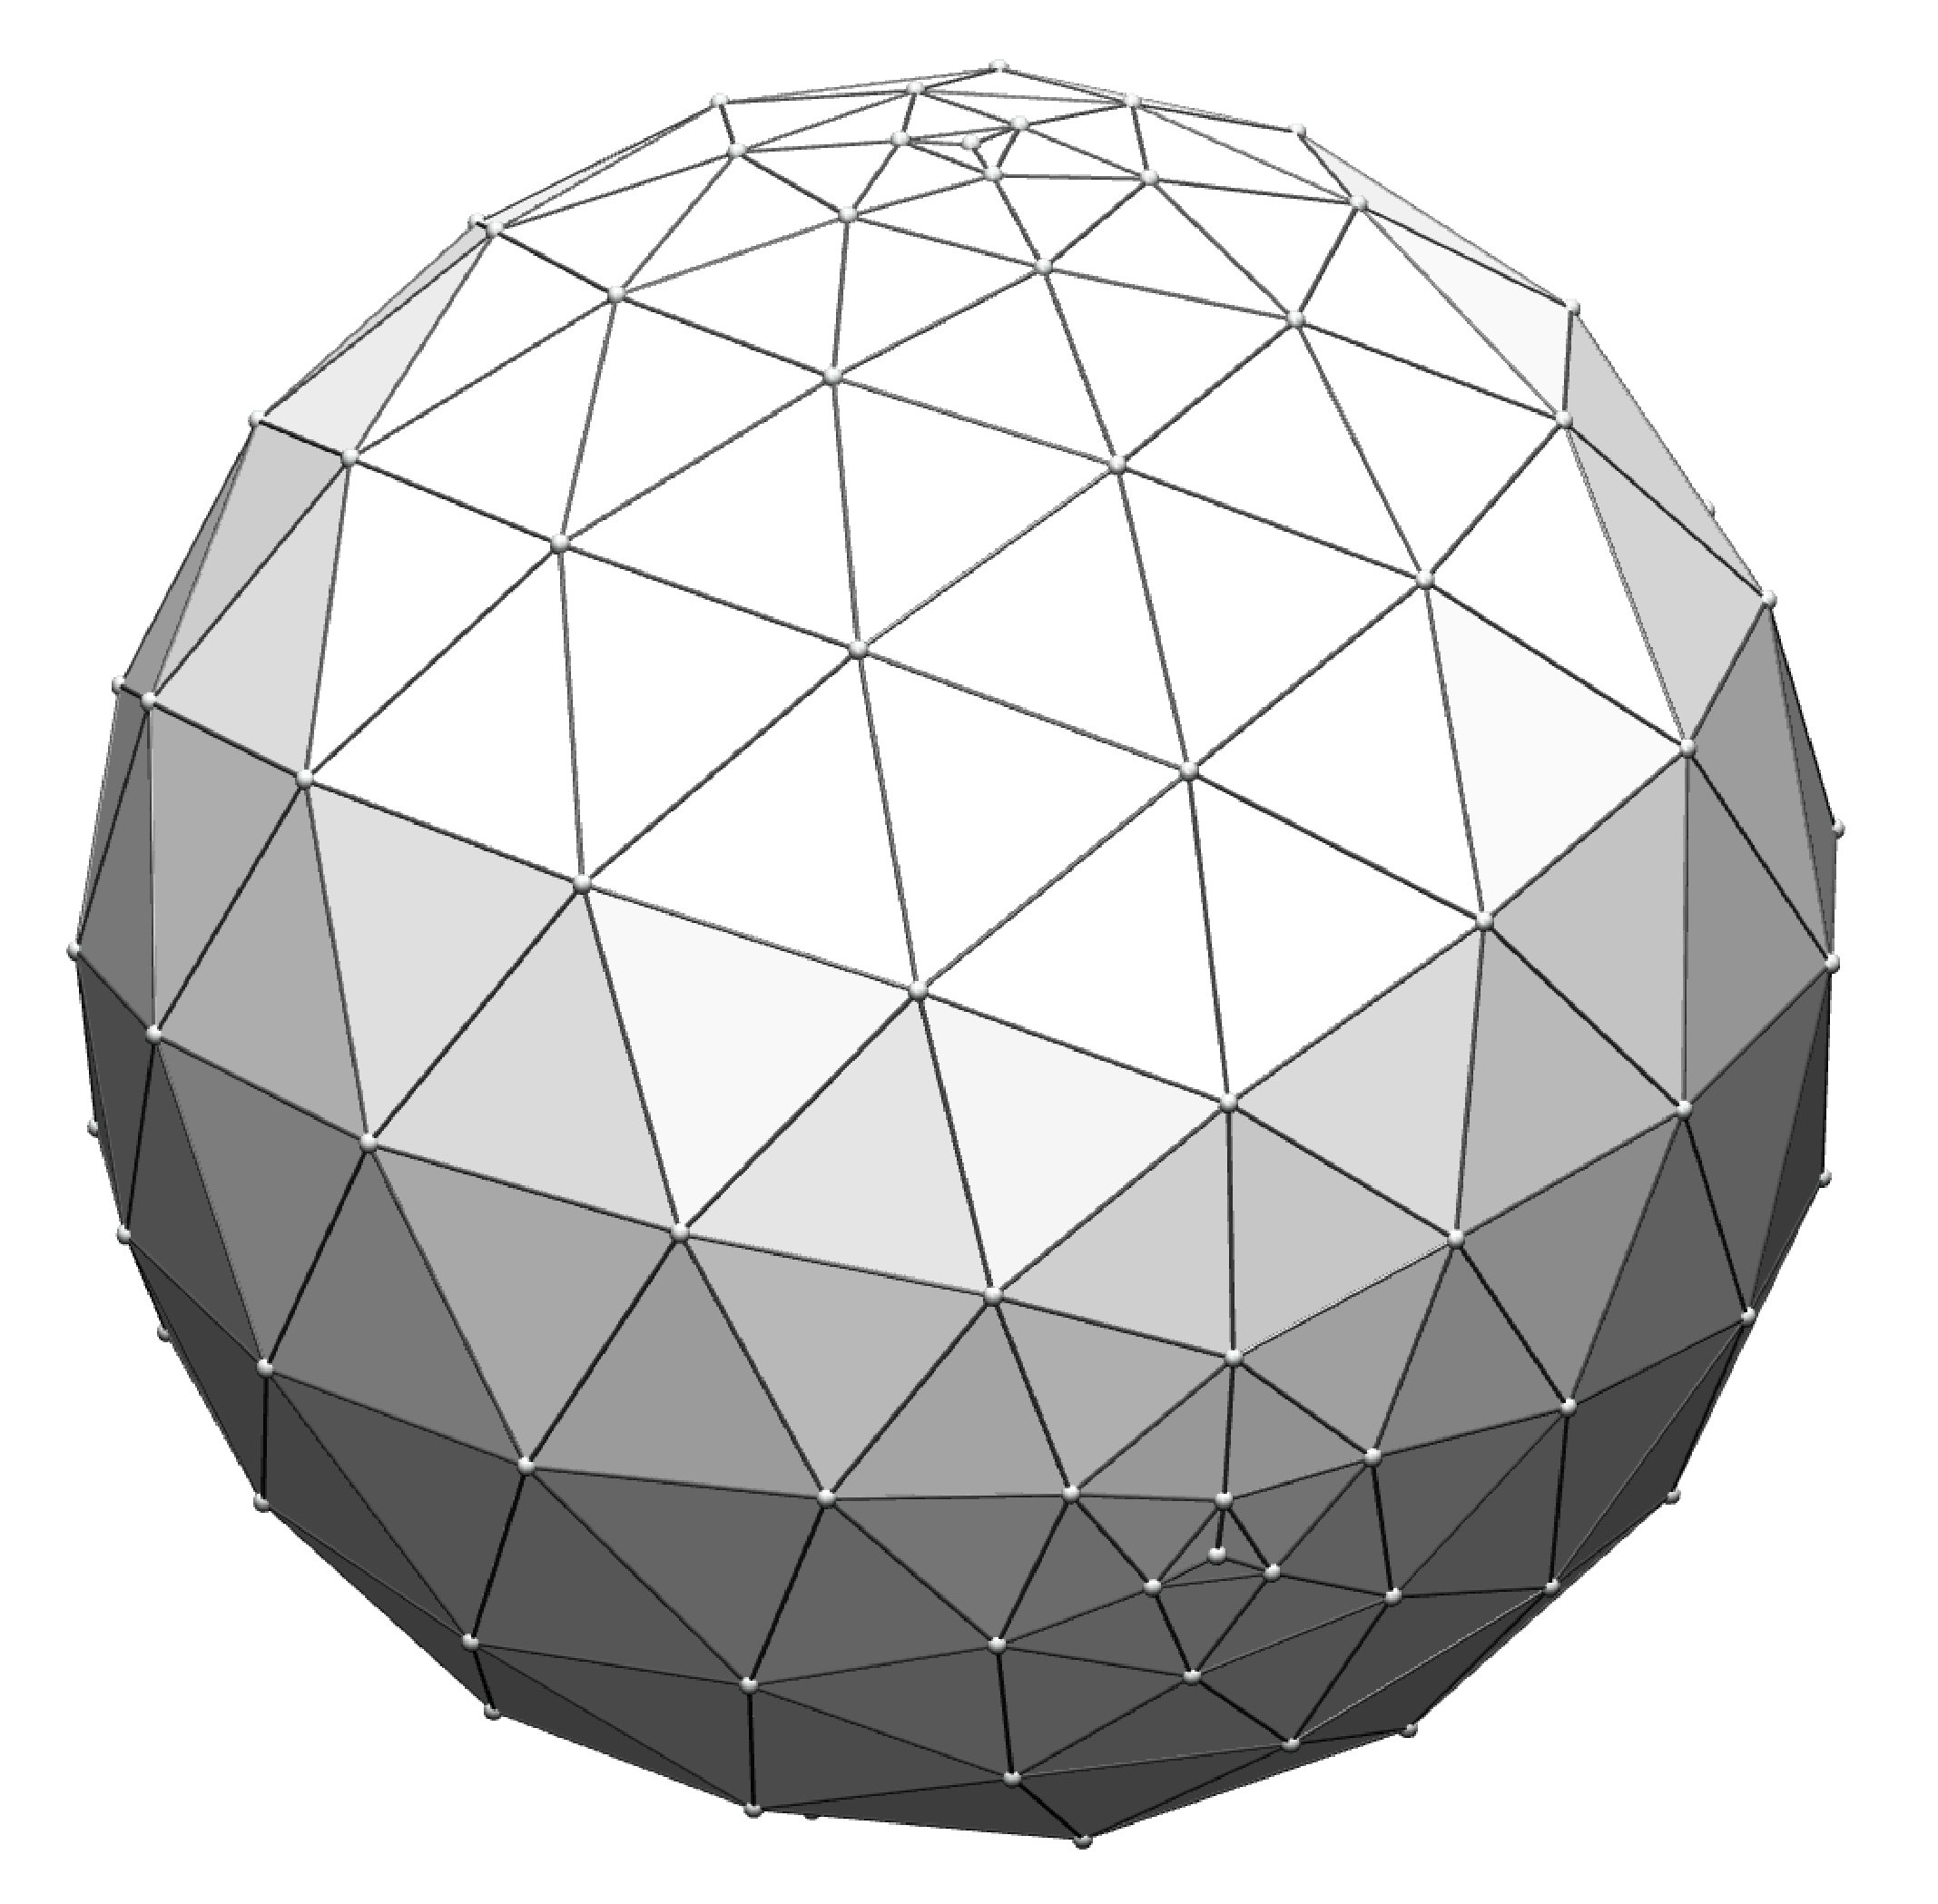
\includegraphics[height=5cm]{spherical/tetrahedron_domain.pdf}
}
\setstretch{0.0}{\scriptsize\tt data/spherical/cube\_data.xml}\quad\quad\quad\quad\quad\quad{\scriptsize\tt data/spherical/tetrahedron\_data.xml}
\caption{Mapping conformally to the sphere using the spherical
  functional. The spherical surfaces are M{\"o}bius-normalized to
  achieve rotational symmetry.}
\label{fig:spherical_examples}
\end{figure}

It is possible to use the spherical functional $E^{\sph}$ to calculate
maps to the sphere even though it is not convex. For simplicity, we
consider only triangulations, so all $\lambda$ variables are fixed and
we may consider $E^{\sph}$ as function of the logarithmic scale
factors $u$ only (see Section~\ref{sec:variational}). A numerical
method has to find a saddle point of $E^{\sph}(u)$. 

Note that the scaling direction $1_{V_{\Delta}}\in\R^{V_{\Delta}}$ is
a negative direction of the Hessian at a critical point: Suppose
$(\Delta,\ell)_{\sph}$ is a spherical triangulation with the desired
angle sum $\Theta_{i}$ at each vertex $i$. Then $0\in\R^{V_{\Delta}}$
is a critical point of $E^{\sph}_{\Delta,\Theta}(u)$. If we enlarge
all edge lengths by a common factor $e^{h}>1$, then all angles become
larger, so every component~\eqref{eq:dEdu} of the gradient of
$E^{\sph}$ becomes negative. Following the negative gradient would
result in even longer lengths.

The following minimax method works in many cases. Define the function
$\tilde E$ by \emph{maximizing} the functional $E^{\sph}$ in the
scaling direction,
\begin{equation}
\label{eq:reduced_spherical}
\tilde E(u)=\max_{h\in\R} \left\{E^{\sph}(u + h1_{V_{\Delta}})\right\}
\end{equation}
Minimize functional $\tilde E$ in a hyperplane of $\R^{V_{\Delta}}$
transverse to the direction $1_{V_{\Delta}}$.

Figure~\ref{fig:intro_uniformization} (top) and
Figure~\ref{fig:spherical_examples} show examples of discrete
conformal maps to polyhedral surfaces inscribed in a sphere that were
calculated using this method.

\subsection{M{\"o}bius normalization}
\label{sec:moebius_normalization}

The notion of discrete conformal equivalence of euclidean polyhedral
surfaces $(\Sigma,\ell)_{\euc}$ in $\R^{3}$ is M{\"o}bius-invariant
(Proposition~\ref{prop:Moebius_inv}). If all vertices $v\in
V_{\Sigma}$ are contained in the unit sphere $S^{2}\subset\R^{3}$,
then there is a M{\"o}bius transformation $T$ of $S^{2}$ such that the
center of mass of the transformed vertices is the
origin~\cite{Springborn05},
\begin{equation*}
\sum_{v\in V_{\Sigma}}T(v) = 0.
\end{equation*}
The M{\"o}bius transformation $T$ is uniquely determined up to
post-composition with a rotation around the origin.

The following method can be used to calculate such a M{\"o}bius
transformation: Find the unique minimizer of the function $\delta$
defined below. Then choose for $T$ a M{\"o}bius transformation that
maps $S^{2}$ to itself and the minimizer to the origin. Here, we only
provide explicit formulas for the function $\delta$ and its first two
derivatives. For a more detailed account, we refer the reader
to Springborn~\cite{Springborn05}. The function $\delta$ is defined on the open
unit ball in $\R^{3}$ by
\begin{equation}
  \delta(x) = \sum_{v\in V}
  \log\left(\frac{-\langle x,v\rangle}{\sqrt{-\langle x,x\rangle}}\right),
\end{equation}
where 
\begin{equation}
  \langle x,y\rangle=x_1y_1+x_2y_2+x_3y_3-1. 
\end{equation}
The gradient and Hessian matrix of $\delta$ are
\begin{align} 
	\operatorname{grad}\delta(x)
        &= \sum_{v\in V}\left(\frac{v}{\langle x,v\rangle} -
          \frac{x}{\langle x,x\rangle}\right),\\
	 \operatorname{Hess}\delta(x)
        &= \sum_{v\in V}\left(2\frac{x^Tx}{\langle x,x\rangle^2}-\frac{v^Tv}{\langle x,v\rangle^2} - \mathrm{diag}\left(\frac{1}{\langle x,x\rangle}\right)\right).
\end{align}

\section{Uniformization of tori}
\label{sec:tori}

Every Riemann surface $R$ of genus one is conformally equivalent to a
flat torus, i.e., to a quotient space $\C/\Gamma$, where
$\Gamma=\Z\omega_{1}+\Z\omega_{2}$ is some two-dimensional lattice
in~$\C$. The biholomorphic map from $R$ to $\C/\Gamma$, or from the
universal cover of $R$ to $\C$, is called a uniformizing map. For a
polyhedral surface of genus one, constructing a discrete uniformizing
map amounts to solving Problem~\ref{prob:total_angles} with prescribed
total angle $\Theta=2\pi$ at all vertices. This provides us with a
method to calculate approximate uniformizing maps for Riemann surfaces
of genus one given in various forms. We consider examples of tori
immersed in $\R^{3}$ in Section~\ref{sec:immersed_tori} and elliptic
curves in Section~\ref{sec:elliptic_curves}. (We will also consider
tori in the form of Schottky uniformization in
Section~\ref{sec:schottky}, as a toy example after treating the higher
genus case.)

The belief that discrete conformal maps approximate conformal maps is
not based on a proven theorem but on experimental evidence like the
Wente torus example of Section~\ref{sec:immersed_tori} and the
numerical experiments of Section~\ref{sec:numerical_convergence}. 

\subsection{Immersed tori}
\label{sec:immersed_tori}

% The conformal classes of flat tori can be parameterized by parallelogram lattices. 
% Two lattices are equivalent if their complex edge ratios $\tau = \frac{\omega_1}{\omega_2}$ agree.
% In this section we describe how to use discrete conformal maps to find analog constructions for discrete cyclic tori, see, e.g., Figure~\ref{fig:intro_uniformization}, middle. 
% We show how to find conformally equivalent flat tori and their corresponding lattices for given polyhedral cyclic tori.

% Section~\ref{sec:tori_schottky} introduces the discrete uniformization of tori given by Schottky data, i.e., a group of loxodromic transformations together with a set of circles in $\Chat$. 
% In Section~\ref{sec:elliptic_curves} we treat tori given as algebraic curves, i.e., elliptic curves. 
% We use elliptic curves to gain insight into the convergence behavior of discrete conformal maps in Section~\ref{sec:numerical_convergence}.

First we consider a simple example with quadrilateral faces.
Figure~\ref{fig:torus_cyclic} (left) shows a coarse discretization of
a torus whose faces are inscribed in circles. On the right, the figure shows the
uniformization obtained by solving Problem~\ref{prob:total_angles}
with prescribed total angle $\Theta=2\pi$ at all vertices.

\begin{figure}%[b]
  \centering
   \includegraphics[height=5cm]{torus_cyclic/torus_cyclic_image.pdf}\\
   \vspace{1mm}
   \includegraphics[width=0.8\textwidth]{torus_cyclic/torus_cyclic_domain.pdf}\\
  \setstretch{0.0}{\scriptsize\tt data/torus\_cyclic/torus\_cyclic.xml} 
  \caption{ Uniformization of an immersed torus with cyclic quadrilateral faces.}
\label{fig:torus_cyclic}
\end{figure}

% Let $(\Sigma, \ell)$ be a cyclic polyhedral surface with genus $1$ without boundary. 
% We solve Problem~\ref{prob:total_angles} to find a euclidean flat metric $\tilde \ell$ with $\Theta_1=2\pi$ for all $i\in V$.
% Once we have a solution we can construct the universal cover of $\Sigma$ by laying out the faces into the plane, see Figure~\ref{fig:torus_cyclic}. We construct the uniformizing group, i.e., the group of translations, using an analogous euclidean procedure as described for surfaces of higher genus in Section~\ref{sec:higher_genus}.

To test the numerical accuracy of our discrete uniformizing maps, we
consider the famous torus of constant mean curvature discovered by
Wente~\cite{wente1986}. Explicit doubly-periodic conformal immersion
formulas (i.e., formulas for the inverse of a uniformizing map) are
known in terms of elliptic functions~\cite{abresch1987, walter1989, bobenko1991}. 

\begin{figure}
\centering
\includegraphics[width=0.48\textwidth]{wente_embedding/wente_1240_fundamental.pdf}\hfill
\includegraphics[width=0.48\textwidth]{wente_embedding/wente_1240_domain.pdf}
\setstretch{0.5}{\scriptsize\tt data/wente\_embedding/wente\_1240.xml}
\caption{Uniformization of the Wente torus. Discretely sampled conformal immersion (left), domain of uniformization (right). Orange curves indicate the lattice of the flat torus in the domain. The faces of the polyhedral surface are approximately conformal squares. In the discrete uniformization their images are approximately squares, as it should be.}
\label{fig:wente_torus_embedded}
\end{figure}

Figure~\ref{fig:wente_torus_embedded} (left) shows a triangulated model 
of the Wente torus constructed by sampling
an explicit immersion formula~\cite{bobenko1991} on a nearly square
lattice containing the period lattice~$\Gamma$. On the right, the
figure shows the discrete uniformization, which reproduces the regular
lattice $\Gamma$ to high accuracy. The modulus
$\tau=\omega_{2}/\omega_{1}$ of the Wente torus has been determined
numerically~\cite{Heil95} as $\tau =
0.41300\ldots+i\;0.91073\ldots$\;. The modulus of the discrete
uniformization of the discretized surface shown in the figure is
$\tilde \tau = 0.41341\ldots + i\;0.91061\ldots$\;.

% As a first test we investigate the behavior of discrete conformal maps on the discretization of a conformal immersion of the Wente torus \cite{wente1986}, Figure~\ref{fig:wente_torus_embedded}. 
% The modulus of the Wente torus has been calculated reliably before \cite{Heil95} as $\tau \approx 0.41300+0.91073i$.
% We calculate a the modulus of the discretized surface as $\tilde \tau \approx 0.41341+0.91061i$, see Figure~\ref{fig:wente_torus_embedded}.

\subsection{Elliptic curves}
\label{sec:elliptic_curves}

An algebraic curve of the form
%\[C=\left\{(\lambda,\mu)\in \C^2 \mid \mathcal P(\lambda,\mu)=0\right\}\]
\begin{equation}
  \label{eq:elliptic_curve}
  \mu^{2}=a\prod_{j=1}^{k}(\lambda-\lambda_{j}),
\end{equation}
where the $\lambda_{j}\in\C$ are distinct and $k=3$ (an elliptic
curve) or $k=4$ (with the singularity at infinity resolved),
represents a Riemann surface of genus one as branched double cover of
the $\lambda$-sphere $\C\mathrm{P}^{1}$, which we identify conformally
with the unit sphere $S^{2}\subset\R^{3}$. The branch points are
$\lambda_{1},\lambda_{2},\lambda_{3},\infty$ if $k=3$ and
$\lambda_{1},\lambda_{2},\lambda_{3},\lambda_{4}$ if $k=4$. Every
Riemann surface of genus one can be represented in this way.

%  where $\mathcal P$ is an
% irreducible polynomial.  This curve in turn can be represented as
% branched covering of the Riemann sphere $\hat{\C}$ with branch points
% at locations $\lambda_i$ with \[\frac{\partial\mathcal P}{\partial
%   \mu}\Bigr|_{\lambda=\lambda_i} = 0.\] In the discrete setting we
% represent discrete algebraic curves as triangulations of the
% respective branched covering of $S^2$.  We only cover 2-sheeted
% coverings here as this includes our main examples, i.e., elliptic
% curves and hyperelliptic curves, see also
% Section~\ref{sec:hyperelliptic}.

We construct a discrete model for a double cover of $S^{2}$ branched
at four points $\lambda_1,\ldots,\lambda_{4}$ in the following way.
Choose $n$ other points $p_1,\ldots,p_n\in S^2$ and let $P$ be the
boundary of the convex hull of the points
$\{\lambda_1,\ldots,\lambda_{4},p_1,\ldots,p_n\}$. Then $P$ is a
convex polyhedron with $n+4$ vertices and with faces inscribed in
circles. (Generically, the faces will be triangles. In
Section~\ref{sec:spherical_triangulations} we explain the method we
used to obtain ``good'' triangles.) Find two disjoint simple edge
paths $\gamma_1,\gamma_{2}$ joining the branch points $\lambda_{j}$ in
pairs. Take a second copy $\hat P$ of the polyhedron $P$. Cut and glue
$P$ and $\hat P$ along the paths $\gamma_1,\gamma_{2}$ to obtain a
polyhedral surface of genus $1$. Uniformize it by solving
Problem~\ref{prob:total_angles}. One obtains a discrete conformal map
to a flat torus, whose inverse can be seen as a discrete elliptic
function. Figure~\ref{fig:p_functions} shows examples. We will treat
hyperelliptic curves in a similar fashion in
Section~\ref{sec:hyperelliptic}.

\begin{figure}
\centering
\resizebox{\textwidth}{!}{
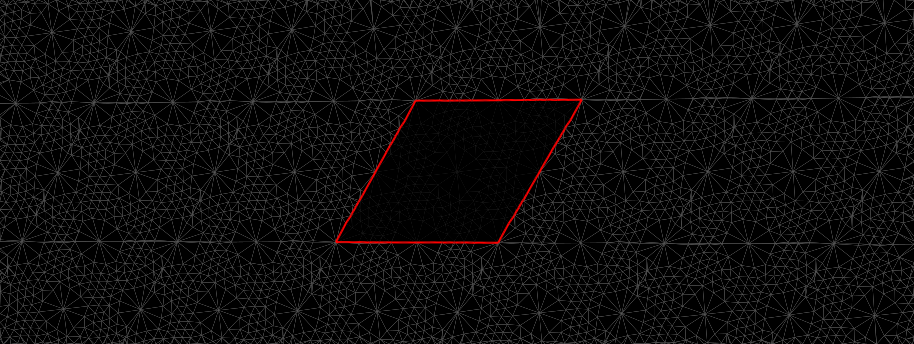
\includegraphics[width=0.5\textwidth]{elliptic_curves/tetrahedron.pdf}
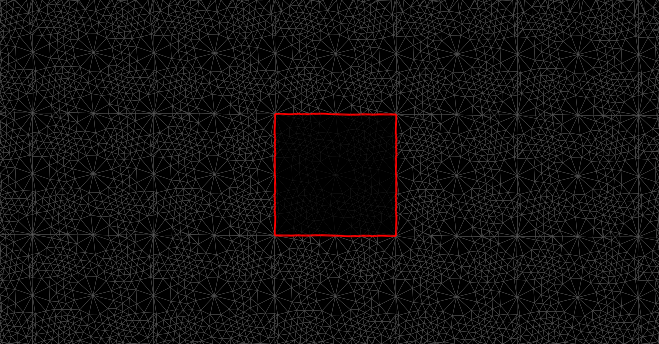
\includegraphics[width=0.5\textwidth]{elliptic_curves/square.pdf}
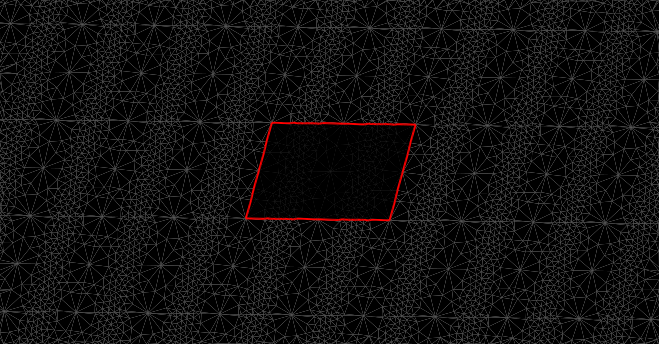
\includegraphics[width=0.5\textwidth]{elliptic_curves/generic.pdf}
}
\setstretch{0.8}{\scriptsize\tt data/elliptic\_curves/\{tetrahedron|square|generic\}.xml}
\caption{Discrete uniformization of elliptic curves. Left: If the
  branch points in $S^{2}$ are the vertices of a regular tetrahedron,
  period lattice is very close to a hexagonal lattice. Middle: If the
  branch points form a square on the equator, the period lattice is
  very close to a square lattice. Right: an example with branch points
  in unsymmetric position.}
\label{fig:p_functions}
\end{figure}

\begin{remark}
  Instead of constructing a doubly-covered convex euclidean polyhedron
  with vertices on the unit sphere as described above, one could also
  construct a spherical triangulation of the doubly-covered sphere
  that is invariant under the elliptic involution (exchanging
  sheets). These two approaches are in fact equivalent due to
  Remark~\ref{rem:chords}. 
\end{remark}

\runinhead{Mapping a flat torus to an elliptic curve.} We can
also go the opposite way, mapping a flat torus to a double cover of
$S^{2}$. Start with a triangulated flat torus. The triangulation
should be symmetric with respect to the elliptic involution, i.e.,
symmetric with respect to a half turn around one vertex (which is then
also a half turn around three other vertices). The quotient space of
the triangulated torus modulo the elliptic involution is then a
triangulated sphere. Map it to the sphere by the procedure explained
by Bobenko {\it et al.}\ \cite[Section 3.2]{BPS2015:dconf}, see also
Section~\ref{sec:spheres_euclidean} of the present work.

Figures~\ref{fig:wente_elliptic} and~\ref{fig:square_elliptic} show
examples where we started with a hexagonal and a square torus
respectively. 

\begin{figure}
\centering
\resizebox{\textwidth}{!}{
\includegraphics[height=4.5cm]{elliptic_tetrahedron_uniform/tetrahedron_uniform_domain.pdf}
\includegraphics[height=4.5cm]{elliptic_tetrahedron_uniform/tetrahedron_uniform_image.pdf}
}
\setstretch{0.8}{\scriptsize\tt data/elliptic\_tetrahedron\_uniform/tetrahedron\_uniform\_branched.xml}
\caption{Mapping the hexagonal torus $\C/(\Z+\tau\Z)$,
  $\tau=\tfrac{1}{2}+i\tfrac{\sqrt 3}{2}$ (left) to a double cover of
  the sphere (right). Because the regular triangulation of the torus
  on the left is symmetric with respect to the elliptic involution,
  its image projects to a triangulation of the sphere seen on the right.} 
\label{fig:wente_elliptic}
\end{figure}

\begin{figure}
\centering
\resizebox{\textwidth}{!}{
\includegraphics[height=4.7cm]{elliptic_square_uniform/square_uniform_fine_domain.pdf}
\includegraphics[height=4.7cm]{elliptic_square_uniform/square_uniform_fine_image.pdf}
}
\setstretch{0.8}{\scriptsize\tt data/elliptic\_square\_uniform/square\_branched.xml}
\caption{ Mapping the square torus $\C/(\Z+i\Z)$ (left) to a double
  cover of the sphere (right). Again, the triangulation on the left
  is symmetric with respect to the elliptic involution, so the image
  on the right projects to a triangulation of the sphere.}
\label{fig:square_elliptic} 
\end{figure}


%\runinhead{Creating good triangulations of the sphere}
\subsection{Choosing points on the sphere}
\label{sec:spherical_triangulations}

The uniformization procedure for elliptic curves described in
Section~\ref{sec:elliptic_curves} requires choosing points on the
sphere in addition to the four given branch points. For numerical
reasons, these points should be chosen so that taking the convex hull
leads to triangles that are close to equilateral. We obtained good
triangulations by minimizing the following energy for $n$ points in
$\R^{3}$ while fixing the subset of branch points:
\begin{eqnarray}
\mathcal E &=& n^2\sum_{v\in V}\left( \left<v,v\right> - 1\right)^2 +
\sum_{\substack{v,w\in V\\w\neq v}} \frac{1}{\left<w-v,
    w-v\right>},
\\ 
\frac{\partial \mathcal E}{\partial v} &=& 4n^2\left<v,v\right>v + 4\sum_{\substack{w\in V\\w\neq v}}\frac{w-v}{\left<w-v,w-v\right>^2}
\end{eqnarray}
where $\left<.,.\right>$ denotes the standard euclidean scalar product
of $\R^{3}$. We do not enforce the constraint that the points should
lie in the unit sphere $S^{2}$. Instead, we simply project back to $S^{2}$
after the optimization.

As initial guess we choose points uniformly distributed in $S^{2}$. To
achieve this we choose points with normally distributed coordinates
and project them to $S^2$~\cite{Muller1959}.


%\runinhead{Numerical experiments}
\subsection{Numerical experiments}
\label{sec:numerical_convergence}

Given the branch points of an elliptic curve, the
modulus $\tau$ can be calculated in terms of hypergeometric
functions. In this section, we compare the theoretical value of $\tau$
with the value $\hat\tau$ that we obtain by the discrete uniformization
method explained in Section~\ref{sec:elliptic_curves}.

% An algebraic curve of genus $g=1$ is called an elliptic curve. We model discrete elliptic curves as described in Section~\ref{sec:elliptic_curves}.

We consider elliptic curves in Weierstrass normal form
\begin{equation}
  \label{eq:Weierstrass_normal_form}
  \begin{split}
    \mu^2
    &=4(z-\lambda_1)(z-\lambda_2)(z-\lambda_3)\\
    &=4z^3-g_2z-g_3,
  \end{split}
\end{equation}
so the branch points $\lambda_{1},\lambda_{2},\lambda_{3},\infty$
satisfy $\lambda_1+\lambda_2+\lambda_3=0$, and 
\begin{equation}
  \label{eq:g-invariants}
  g_{2}=-4(\lambda_1\lambda_2+\lambda_2\lambda_3+\lambda_3\lambda_1),
  \qquad 
  g_{3}=4\lambda_1\lambda_2\lambda_3.
\end{equation}
We calculate the modulus $\tau$ with Mathematica using the built-in
function
\texttt{Wei\-er\-strass\-Half\-Pe\-ri\-ods[$\{g_2,g_3\}$]}. We
normalize $\tau$ and the value $\hat\tau$ obtained by discrete
uniformization so that they lie in the standard fundamental domain of
the modular group, $|\tau|>1$ and $|\re(\tau)| < \frac{1}{2}$, and we
consider the error $|\tau-\hat \tau|$. (We stay away from the boundary
of the fundamental domain.)

% The goal of this section is to provide insights into the convergence behavior of discrete uniformization as presented above. In particular we look into the convergence of period matrices as the number of points that approximate a given Riemann surface increases. For genus one algebraic curves we can calculate period matrices explicitly using the invariants $\{g_2,g_3\}$ of the elliptic surface. Let $\lambda_1,\lambda_2,\lambda_3,\lambda_4\in\C$ be the branch points of the curve such that $\lambda_1+\lambda_2+\lambda_3=0$ and $\lambda_4=\infty$. Then the curve is given as
% \begin{eqnarray*}
% \mu^2&=&4(z-\lambda_1)(z-\lambda_2)(z-\lambda_3)\\
% &=&4z^3+4(\lambda_1\lambda_2+\lambda_2\lambda_3+\lambda_3\lambda_1)z - 4\lambda_1\lambda_2\lambda_3\\
% &=&4z^3-g_2z-g_3.
% \end{eqnarray*}
% The period matrix $[\tau]$, also called the modulus of the curve, can be calculated using the periods of the elliptic lattice $\{\omega_1,\omega_3\}$ such that $\tau = \frac{\omega_2}{\omega_1}$. These can be calculated from the invariants $\{g_2,g_3\}$, e.g., using {\sc Mathematica}s built-in function {\tt WeierstrassHalfPeriods[$\{g_2,g_3\}$]}~\cite{WeierstrassHalfPeriods_website}.

% Let $\lambda_1, \lambda_2, \lambda_3, \lambda_4 \in \C$ be the branch points of an elliptic curve $C$. We create a discrete version of the curve by choosing $n$ points $p_1,\ldots,p_n$ equally distributed on $S^2$. The triangulation for one sheet of the discrete curve is the convex hull of $\{\lambda_1,\ldots,\lambda_4,p_1,\ldots, p_4\}$. Choose non-intersecting edge-paths connecting the pairs $(\lambda_1,\lambda_2)$ and $(\lambda_3,\lambda_4)$. To create a doubly-covered sphere we glue a second copy of the triangulated sphere transversely along corresponding paths, see Section~\ref{sec:elliptic_curves}.

% After discrete uniformization we calculate $\hat \tau$. We normalize $\tau$ and $\hat \tau$ such that $|\tau|>1$ and $|\re(\tau)| < \frac{1}{2}$. We can now compare the modulus $\tau$ of the smooth structure with the number $\hat \tau$ derived from the discrete uniformization of a triangulation with the same branch points. The discretization error is defined as $|\tau-\hat \tau|$.

\runinhead{Subdivided icosahedron.}

In this experiment we start with the twelve vertices of a regular
icosahedron and choose the branch points $\lambda_1,\ldots,\lambda_4$
among them. The remaining points act the role of $p_1,\ldots,p_n$. To study
the dependence of $|\tau-\hat \tau|$ on the number of points we
repeatedly subdivide all triangles into four similar triangles
and project the new vertices to $S^2$. The number of vertices
grows exponentially while the triangles remain close to equilateral.
Figure~\ref{fig:convergence_subdivision} shows the result of this
experiment. It suggests the error behaves like
\begin{equation}
\label{eq:error_ico}
|\tau-\hat \tau|=\mathcal O (n^\alpha),\quad\alpha \approx -0.88.
\end{equation}


\begin{figure}
\centering
\resizebox{\textwidth}{!}{
\includegraphics[width=0.35\textwidth]{convergence/icosubdivision01.pdf}\hfill
\includegraphics[width=0.32\textwidth]{convergence/icosubdivision01_example01.pdf}
}
{\scriptsize\tt data/convergence/subdivision/icosubdivision01.dat}\\
{\scriptsize\tt data/convergence/subdivision/data/icosubdivision01.xml}
\caption{Left: Error for zero to six subdivision steps. The
  $\log$-$\log$ plot shows the error $|\tau - \hat\tau|$ against the
  number of vertices of the subdivided icosahedron (i.e., in one sheet
  of the doubly-covered sphere). To estimate the asymptotic behavior
  of the error, we determine the slope $\alpha\approx-0.88$ of a line
  through the last four points by linear regression. Right: Result of
  the discrete uniformization after two subdivision steps.}
\label{fig:convergence_subdivision}
\end{figure}

\runinhead{Dependence on mesh quality.}

In the second experiment we choose the additional points randomly to
analyze how the quality of the triangulation affects the approximation
error. We use the following quantities to measure the quality of the
triangulation based on length cross-ratios for edges:
\begin{eqnarray*}
	Q_{\lcr}(e) &\vcentcolon=& \frac{1}{2}\left(\lcr(e) + \frac{1}{\lcr(e)}\right) - 1\label{eq:quality_lcr},\\
	Q_{\lmr}(f) &\vcentcolon=& \frac{1}{2}\left(\lmr(f) + \frac{1}{\lmr(f)}\right) - 1\label{eq:quality_lmr},
\end{eqnarray*}
where $\lcr$ denotes the length cross-ratio~\eqref{eq:lcr} of an edge,
and $\lmr$ denotes the length multi-ratio defined for faces by
$\lmr(f)=\prod_{e \in f}\lcr(e)$. If $Q_{\lcr}=0$ for all edges, then
the mesh is discretely conformally equivalent to a mesh consisting of
equilateral triangles. So less is better for these quality
measures. To get enough ``good'' triangulations in our samples, we
improve random meshes with the procedure described in
Section~\ref{sec:spherical_triangulations}.

Figure~\ref{fig:convergence_quality} (left) shows a plot of $2600$
triangulations ranging from $n=20$ to $n=1500$ vertices. No clear
convergence rate is discernible. The situation improves when only
samples with a certain minimal mesh quality are considered.  For the
plot in Figure~\ref{fig:convergence_quality} (right) we selected only
triangulations with $\max_e \{Q_{\lmr}(e)\} < 0.3$. (The results
are similar when using the quality measures $\max_e \{Q_{\lcr}(e)\} <
x$ or $\mean_e \{Q_{\lcr}(e)\} < x$.)

\begin{figure}
\centering
\includegraphics[width=\textwidth]{convergence/quality_rand_points01_maxmultiratio_2.pdf}
\setstretch{0.0}{\scriptsize\tt data/convergence/numberofpoints/quality\_rand\_points01.dat}
\caption{Left: $\log$-$\log$ plot of the error $|\tau - \hat\tau|$
  against the number of vertices for a sample of optimized random
  triangulations with no quality constraint. Right: Only
  triangulations with $\max_e \{Q_{\lmr}(e)\} < 0.3$ are
  considered. The regression line with slope $\alpha\approx -0.63$ is
  shown in red.}
\label{fig:convergence_quality}
\end{figure}

The results from these two experiments suggest that the error depends
on the number of vertices asymptotically like $n^{\alpha}$,
where the exponent $\alpha<0$ depends on the mesh. 

\subsection{Putting a square pattern on a spherical mesh}
\label{sec:square_pattern}

We can use a variant of the discrete uniformization of elliptic curves
(Section~\ref{sec:elliptic_curves}) to put a square pattern on a
surface that is homeomorphic to a sphere.  Figure~\ref{fig:bear} shows
an example.
\begin{figure}
\centering
\resizebox{\textwidth}{!}{
  \includegraphics[height=0.25\textwidth]{bear_torus/baer_quads.pdf}%
  \includegraphics[height=0.25\textwidth]{bear_torus/baer_cuts.pdf}%
  \hspace{1mm}%
  \includegraphics[height=0.25\textwidth]{bear_torus/cover_triangulation_rectangle.pdf}%
  \hspace{1mm}%
  \includegraphics[height=0.25\textwidth]{bear_torus/cover_triangulation.pdf}%
  }
  \setstretch{0.8}{\scriptsize\tt data/bear\_torus/bear60.xml}
  \caption{The discrete ``Berlin Buddy Bear'', a mascot of the
    SFB/Transregio 109 ``Discretization in Geometry and Dynamics''. 
    The square pattern is put on a bear model as described in
    Section~\ref{sec:square_pattern}. Four ramification vertices (marked
    in red) are chosen at the paws. The uniformization of the branched
    double cover is shown in the middle. Each fundamental domain
    covers the bear twice. Fundamental domains of the
    group generated by rotations around the branch points are shown on
    the right. Each covers the bear once.
    % The singularities can be interpreted as branch points
    % of a two-sheeted cover of the bear forming a topological torus.  The
    % corresponding universal cover is generated by euclidean
    % translations, the fundamental domain can be chosen to be an
    % approximate rectangle, middle.  The group of translations is a
    % subgroup of the group generated by the rotations around the
    % singularities about and angle of $\pi$. In a fundamental domain the
    % branch vertices lie in the middle of edges, right.  
  }
  \label{fig:bear}
\end{figure}

Pick four vertices of the mesh as ramification points and create a
two-sheeted branched cover of the mesh by gluing two copies along
paths connecting the selected vertices. The resulting surface is a
torus. It can be uniformized using the euclidean functional. The
uniformizing group is generated by two translations.  This group is a
subgroup of the group generated by rotations around the branch
vertices.  Hence we can achieve the same result as follows. Instead of
doubling the surface, prescribe total angles $\Theta=\pi$ at the
ramification vertices and $\Theta=2\pi$ at all other vertices. The
result is a flat surface with four cone-like singularities of
cone-angle $\pi$. The monodromy of the developing map is generated by
half-turns. Avoiding the double cover is more efficient because one
only has to minimize a function of (approximately) half the number of
variables.

\section{Uniformization of surfaces of higher genus}
\label{sec:higher_genus}

As in the case of tori (Section~\ref{sec:tori}), we can find
uniformizing maps for cyclic polyhedral surfaces of genus $g\geq 2$ by
solving the hyperbolic version ($\gt=\hyp$) of
Problem~\ref{prob:total_angles} with prescribed total angle
$\Theta=2\pi$ at all vertices. (We will only consider
triangulations in the following.)  This allows us to calculate approximate
uniformizations for Riemann surfaces of genus $g\geq 2$ given in
various forms, by approximating them with polyhedral surfaces. 

In Section~\ref{sec:polygons_generators}, we briefly discuss how to
construct fundamental polygons and group generators.

Not much needs to be said about the uniformization of immersed
surfaces. Examples are shown in Figures~\ref{fig:intro_uniformization}
(bottom) and \ref{fig:embedded_genus_3}.
%, and~\ref{fig:embedded_genus_5}.
\begin{figure}
\centering
\resizebox{\textwidth}{!}{
\includegraphics[height=0.4\textwidth]{genus3/genus3.pdf}%
\includegraphics[height=0.4\textwidth]{genus3/canonical_mesh.pdf}%
\includegraphics[height=0.4\textwidth]{genus3/canonical_cover.pdf}
}
\setstretch{0.5}{\scriptsize\tt data/genus3/data.xml}
\caption{Discrete uniformization of an embedded triangulated surface
  of genus $3$. A fundamental polygon with ``canonical'' edge pairing
  is shown on the right together with the image mesh. The edges of the
  polygon (brown) and the axes of the edge-pairing translations (blue)
  are pulled back to the embedded surface shown on the left.}
\label{fig:embedded_genus_3}
\end{figure}
%\begin{figure}
%\centering
%\includegraphics[height=0.4\textwidth]{genus5/genus5.pdf}
%\includegraphics[height=0.4\textwidth]{genus5/fundamental.pdf}\\
%\setstretch{0.5}{\scriptsize\tt data/genus5/data.xml}
%\caption{Left: An embedded triangulated surface of genus $5$. Right:
%  Fundamental polygon with non-canonical edge-pairing. The axes of the
%  edge pairing translations are shown in blue.}
%\label{fig:embedded_genus_5}
%\end{figure}
In Section~\ref{sec:circle_domains} we discussed mappings from
multiply connected domains to circle domains. Analogously, one can
construct uniformizations of polyhedral surfaces of genus $g\geq 2$
with holes over the hyperbolic plane with circular holes. An example
is shown in Figure~\ref{fig:hyperbolic_circle_domain}. More precisely,
the holes are bounded by hyperbolic polygons with vertices on a
circle. 
\begin{figure}
\centering
\resizebox{\textwidth}{!}{
\raisebox{0.75cm}{
\includegraphics[height=3.5cm]{circle_domain_hyperbolic/brezel_three_holes_edges.pdf}
}
\includegraphics[height=5cm]{circle_domain_hyperbolic/brezel_three_holes_domain.pdf}
}
\setstretch{0.0}{\scriptsize\tt data/circle\_domain\_hyperbolic/brezel\_\{one,two,three\}\_holes.xml}
\caption{ Uniformization of a genus-$2$ surface with three boundary
  components over the hyperbolic plane with three circular holes. The
  three holes are filled with polygons, which are then triangulated
  during the calculation, see Sections~\ref{sec:circle_domains}
  and~\ref{sec:vari-princ}.  }
\label{fig:hyperbolic_circle_domain}
\end{figure}

We explain how to calculate the Fuchsian uniformization for Riemann
surfaces given in the form of a Schottky uniformization in
Section~\ref{sec:schottky}. We discuss the uniformization of
hyperelliptic curves in Section~\ref{sec:hyperelliptic} and a
geometric characterization of hyperelliptic Riemann surfaces in
Section~\ref{sec:hyperelliptic_domain}. 

% In this section we describe how to calculate uniformizations of cyclic polyhedral surfaces of higher $g>1$ genus. 
% In particular we show how to construct the corresponding Fuchsian groups and fundamental domains in Section~\ref{sec:fundamental_domains}.
% We revisit surfaces given by Schottky data in Section~\ref{sec:schottky} for genus $g>1$, see also Section~\ref{sec:tori_schottky} for Schottky uniformizations of tori.
% Finally, in Section~\ref{sec:hyperbolic_circle_domain} we construct hyperbolic circle domains analogously to the constructions presented in Section~\ref{sec:circle_domains} for topological spheres or disks.

\subsection{Fundamental polygons and group generators}
\label{sec:polygons_generators}

\runinhead{Basic facts and notation.}
Every compact Riemann $R$ of genus $g\geq 2$ can be represented as the
quotient of the hyperbolic plane $H^{2}$ modulo the action of a discrete
group~$G$ of hyperbolic translations,
\begin{equation}
R=H^{2} / G.
\end{equation}
Presentations of the group $G$ play an important role. We will denote
generators by capital letters and their inverses by primes,
\begin{equation}
  A'\vcentcolon=A^{-1}\in G.
\end{equation}
The uniformization group $G$ can be presented with a finite set of
generators 
\begin{equation*}
A,B,C,D,\ldots\in\operatorname{Isom}(H^{2})
\end{equation*}
subject to a single relation $r=1$,
\begin{equation}
G=\left<A,B,C,D,\ldots\mid r=1\right>,
\end{equation}
where $r$ is a product in which all generators and their inverses
appear exactly once. Such presentations are closely related with
fundamental polygons: Every fundamental polygon in which all vertices
are identified leads to such a presentation.

A fundamental domain of $G$ is an open connected subset $D$ of the
hyperbolic plane such that the $G$-orbit of the closure $\bar D$
covers $H^{2}$, and $gD\cap D=\emptyset$ for all $g\in
G\setminus\{1\}$.  A fundamental polygon of $G$ is a fundamental
domain with polygonal boundary, i.e., the boundary consists of
geodesic segments, the \emph{edges} of the fundamental polygon, which
are identified in pairs by the action of the group $G$. For each edge
$a$, there is exactly one partner edge $a'$ such that there exists a
translation $A\in G$ mapping $a$ to $a'$. These edge-gluing
translations form a generating set of $G$. If all vertices of the
fundamental polygon are identified (i.e., they belong to the same
$G$-orbit), then the fundamental polygon has $4g$ edges. In this case
there is only one relation for these generators. The relation can be
determined from the edge labels, which we always list in
counterclockwise order. For example, if the edges of an octagon are
labeled ``canonically'',
\begin{equation}
\label{eq:canonical_polygon}
aba'b'cdc'd',
\end{equation}
then the relation for the corresponding edge pairing
translations is 
\begin{equation}
  \label{eq:canonical_relation_g2}
  DC'D'CBA'B'A, 
\end{equation}
and if opposite edges are identified,
\begin{equation}
  \label{eq:opposite_polygon_g2}
  abcda'b'c'd', 
\end{equation}
the relation is 
\begin{equation}
\label{eq:opposite_relation_g2}
DC'BA'D'CB'A=1.
\end{equation}

\runinhead{Computational aspects.}
%\subsection{Computation of fundamental domains and Fuchsian groups}
%\label{sec:fundamental_domains}

\begin{figure}
\centering
(a)\includegraphics[height=0.42\textwidth]{algorithm/step1_boundary.pdf}
(b)\includegraphics[height=0.42\textwidth]{algorithm/step2.pdf}
\\
(c)\includegraphics[height=0.42\textwidth]{algorithm/step3.pdf}
(d)\includegraphics[height=0.42\textwidth]{algorithm/contract_combined.pdf}
\\
(e)\includegraphics[height=0.42\textwidth]{algorithm/step5.pdf}
(f)\includegraphics[height=0.42\textwidth]{algorithm/step5_5.pdf}
\setstretch{0.0}{\scriptsize\tt data/algorithm/data.xml}
\caption{ Constructing a fundamental polygon with opposite edges
  identified.  (a) Laying out hyperbolic triangles creates a
  fundamental polygon with many vertices. (b) Straighten the edges
  between vertices that are identified with more than one partner
  (shown in red). (c) Axes of the edge-pairing translations are shown
  in blue. (d,e) Two cut-and-paste operations lead to a fundamental
  polygon with one vertex class and opposite edges identified. The
  axes intersect in one point (see
  Section~\ref{sec:hyperelliptic_domain}). We move this point to the
  origin. (f) Tiling the hyperbolic plane with fundamental polygons.}
\label{fig:fundamental_polygon_algorithm}
\end{figure}

Let $(\Sigma,\ell)$ be a closed (euclidean, spherical, or
hyperbolic) triangulated surface of genus $g\geq 2$. We solve
Problem~\ref{prob:total_angles} to obtain a combinatorially equivalent
hyperbolic triangulated surface $(\Sigma,\ellt)_{\hyp}$ with angle sum
$\Theta=2\pi$ at every vertex. We lay out the triangles in the
hyperbolic plane one-by-one, following a breadth-first search of the
the $1$-skeleton of the dual cell complex of
$\Sigma$. (Alternatively, one could use a shortest spanning tree of
the $1$-skeleton of the dual complex~\cite{EricksonH02}.) The result is a
fundamental polygon with many vertices. An example is shown in
Figure~\ref{fig:fundamental_polygon_algorithm} (a).

We simplify this fundamental polygon by connecting vertices that are
identified with more than one partner by geodesic arcs, as shown in 
Figure~\ref{fig:fundamental_polygon_algorithm} (b). The resulting
polygon has in general more than one vertex class.

Now we perform the standard algorithm involving cut-and-glue
operations (see, e.g.,~\cite{Jost2007}) to obtain a fundamental
polygon with one vertex class and so-called canonical edge
identification 
\begin{equation}
aba'b'cdc'd'\ldots\;. 
\end{equation}
During this process we maintain
edge-identification transformations, which we represent as
$SO^{+}(2,1)$ matrices. 

Hyperbolic translations tend to accumulate numerical errors quite fast when
building products. The situation could be ameliorated somewhat by using
the $PSL(2,\R)$-representation of hyperbolic
isometries~\cite{Floyd2002}, but the fundamental problem remains. For
this reason, it is desirable to perform the cut-and-glue algorithm in
such a way that the number of matrix products required to maintain the
gluing translations is small. 

%We follow the following greedy
%approach. Repeatedly we have to choose labels $x$, $y$ such that the
%order in the polygon is $x\cdots y\cdots x'\cdots y'$, and then
%perform a cut-and-glue sequence to bring the labels next to each
%other, $xyx'y'$. We always choose a pair $x$, $y$, for which this
%requires the minimal number of matrix multiplications.
%
%\runinhead {Canonical Fundamental Domain.}

\begin{figure}
\centering
\resizebox{0.4\textwidth}{!} {
\input{data/algorithm/cutCanonical.pdf_t}
}
\caption{Cut-and-paste: Cut from the start of $a$ to the start of side $b$. Glue the piece along $a'$ using transformation $A$ that moves side $a$ to $'a$. Intermediate sides $c_1,\ldots,c_n$ between $a$ and $b$ are transformed accordingly and group elements transform as $\hat{C_i}=C_iA'$. Their inverses $C_i'$ become $\hat{C_i}'=AC_i'$}
\label{fig:cut-and-paste-canonical}
\end{figure}

 \begin{figure}
 \centering
 \resizebox{\textwidth}{!}{
 \includegraphics[width=5cm]{algorithm/canonical_step0_labels.pdf}
 \includegraphics[width=5cm]{algorithm/canonical_step1_labels.pdf}
 \includegraphics[width=5cm]{algorithm/canonical_step2_labels.pdf}
 }
 \caption{Motions to transform a given fundamental domain into canonical form. The shaded area is the current fundamental polygon. Step~$1$: Choose the linked pair $a$, $b$. Cut at $c$ and $b$ and identify via $B$ to put side $a$ next to side $b$. Choose linked pair $e$, $f$. Cut between $e'$ and $d'$ and identify via $E'$ to put side $e'$ next to $f'$. The remaining handle $cdc'd'$ is already in place and we arrive at canonical form $aba'b'cdc'd'efe'f'$.}
 \label{fig:canonical_algorithm}
 \end{figure}

 We start with a fundamental polygon with a single vertex class that is not in canonical form. 
 Then choose sides $a$ and $b$ such that the order in the polygon is $a\cdots b \cdots a' \cdots b' \cdots$. 
 We perform a cut-and-paste operation such that sides $a$ and $b$ are next to each other after transformation, see Figure~\ref{fig:cut-and-paste-canonical}. 
 In order to minimize the number of products we choose $a$ and $b$ such the number of sides in between $a$, $b$, $a'$, and $b'$ is minimal. 
 We proceed cutting as described before to bring $b$ next to $a'$ and analogously $a'$ next to $b'$. 
 We end up with a new polygon and the order $aba'b'\cdots$. 
 Repeat this algorithm for the rest of the sides to arrive at canonical form. 
 Again a proof can be found, e.g., in the book by Jost~\cite{Jost2007}.
 See Figure~\ref{fig:canonical_algorithm} for an example of this algorithm.

 The number of products built during the transformation of a linked pair $a$, $b$ depends on the number of polygon sides between $a$, $b$, $a'$, and $b'$. 
 Let $C$ be the number of sides between $a$ and $b$. Let $D$ and $E$ be the number of sides between $b$, $a'$, and $b'$ respectively. 
 Then the total number of products in this transformation is $6C+4D+2E$. 
 In step $1$, connecting $a$ and $b$, we can perform the cut-and-past operation using transformation $b$ and a cut between the end of $a$ and the end of $b$ in counter-clockwise order. 
 This moves the intermediate sides between $a$ and $b$ out of the way for the next $2$ steps. 
 By this we have a total number of products $2C+4D+2E$. 
 We use a greedy implementation that chooses the smallest number of products in each step to select $a$ and $b$.
 Alternatively one could enumerate the transformation tree and choose the cheapest path of all transformation sequences.


The polygon with canonical edge identifications may not be
convex. Following Linda Keen~\cite{keen1966}, we can transform this domain
into a strictly convex fundamental polygon by choosing a different
base vertex for the same group of transformations. Let
$aba'b'cdc'd'\ldots$ be a fundamental polygon and let
\begin{equation}
G=\left<A,B,C,D,\ldots\in \mathit{PSL}(2,\R)\mid \ldots DC'D'CBA'B'A =1\right>
\end{equation}
be the corresponding presentation of the uniformization group, see
Figure~\ref{fig:keen_polygon} (left). Then the axes of the generators
$A$ and $B$ intersect in a point $p_0$. Choosing $p_0$ as the base
point of a new fundamental polygon as shown in
Figure~\ref{fig:keen_polygon} (right) renders it convex and uniquely
determined for the given group and presentation.
\begin{figure}
\centering
\resizebox{0.8\textwidth}{!}{
\includegraphics[width=5cm]{keen/canonical01_labels.pdf}
\includegraphics[width=5cm]{keen/keen01_labels.pdf}
}
\caption{ The algorithm of Linda Keen to construct strictly convex
  fundamental polygons.  Start with any canonical fundamental polygon
  $aba'b'cdc'd'$ with a corresponding relation $DC'D'CBA'B'A=1$
  (left).  We choose the intersection $p_0$ of the axes of
  transformations $A$ and $B$ as base point for the new domain. The
  new vertices of the fundamental domain are calculated as
  $p_1=A'Bp_0$, $p_2=A'p_0$, $p_3=Bp_0$, and
  $p_4=BA'p_0$.  The other vertices are obtained similarly from $p_4$
  by applying~$C$ and~$D$.}
\label{fig:keen_polygon}
\end{figure}

\runinhead{Fundamental polygons with opposite sides identified.}

When we consider the geometric characterization of hyperelliptic
surfaces in Section~\ref{sec:hyperelliptic_domain}, we want to
transform fundamental polygons into fundamental polygons with opposite
sides identified, i.e., polygons with edge labeling 
\begin{equation*}
abcd\cdots a'b'c'd'\cdots.
\end{equation*}
Any fundamental polygon can be transformed into a fundamental polygon
with opposite edges identified by cut-and-glue operations: First
transform the polygon to canonical form $aba'b'cdc'd'\ldots$ by the
standard algorithm. Playing a sequence of steps that transforms
a polygon with opposite edges identified to canonical form backwards,
transforms the canonical polygon to a polygon with opposite edges
identified.

This algorithm is not optimal with respect to the number of
multiplications necessary to maintain the edge-gluing
translations. Especially if the original polygon is already ``close''
to one with opposite sides identified, the detour via a canonical
polygon is inefficient.  

In all examples, we use a heuristic method based on the following
idea: Find one of the longest sequences of different letters in the edge
labeling (ignoring primes), and then try to move a different letter
into this sequence by cutting and gluing.

 \begin{figure}
 \resizebox{\textwidth}{!}{
 \includegraphics[width=5cm]{algorithm/opposite_step0_labels_start.pdf}
 \includegraphics[width=5cm]{algorithm/opposite_step0_labels.pdf}
 \includegraphics[width=5cm]{algorithm/opposite_step1_labels.pdf}
 }
 \resizebox{0.666666\textwidth}{!}{
 \includegraphics[width=5cm]{algorithm/opposite_step2_labels.pdf}
 \includegraphics[width=5cm]{algorithm/opposite_step3_labels.pdf}
 }
 \caption{Algorithm example: Start with group relation $B'F'D'E'A'FEC'DCBA = 1$. Step~$1$: Cut from the start of $d'$ to the end of $c'$ and identify via $C'$ to move $C'$ behind $D'$. The resulting relation is clustered such that the elements of the first half form the inverses of the second half: $B'F'D'C'E'A'FEDCBA= 1$. We now sort elements $A,\ldots,B$ to match the order of $A',\ldots,F'$ or vice versa. Step~$2$: Cut at $a'$ and $b$ and identify via $B$ to move $B$ behind $A'$. We get relation $B'F'D'C'E'A'BFEDCA = 1$. Step~$3$: Cut between $d'$ and $e$ and identify via $E$ to move $E$ behind $C$. We get $B'F'D'C'E'A'BFDCEA = 1$ as the final relation and a fundamental polygon with oppositely identified sides.}
 \label{fig:opposite_algorithm}
 \end{figure}

 \begin{figure}
 \centering
 \resizebox{0.3\textwidth}{!} {
 \input{data/algorithm/moveElement.pdf_t}
 }
 \caption{Move element $A$ in front of $B$ in a relation that moves counter-clockwise around the base vertex. Choose the upper cut (dashed lines) and paste via transformation $A'$ moving side $a'$ to $a$. Or cut at the lower one and paste via transformation $A$.}
 \label{fig:cut-and-paste-motion}
 \end{figure}
%
% A fundamental polygon identified by opposite sides has a side ordering
% \begin{equation*}
% abcd\cdots a'b'c'd'\cdots.
% \end{equation*} 
% A corresponding relation of the group of hyperbolic translations is $AB'CD'\cdots=1$ given that a transformation $X$ maps side $x$ to $x'$.
%
% We give two algorithms to transform a given fundamental domain into an opposite sides domain.
% For the first algorithm we show that it terminates and yields the correct result. However we cannot control the number of products used during the transformation. The second algorithm is heuristic and minimizes the number of products. It has proven to terminate for all of our examples.
%
% We use the canonical form of fundamental polygons as an intermediate step in the process of transforming a given fundamental domain into opposite sided form. As shown above we can transform any domain into canonical form. In particular we can transform an abstract oppositely identified polygon into canonical form using the algorithm from above. All of the steps conducted during this transformation can be undone. We get a sequence of cut-and-paste operations transforming a canonical fundamental polygon into opposite sides form. Combining the sequence that transforms a general fundamental polygon into canonical form with the transform that creates the opposite form from the canonical one we get required sequence on transformations on any given domain.
%
% This version of the algorithm is not optimal with respect to the number of products used in the sequence of transformations. In particular if the input polygon is close to opposite sides form already, the algorithm destroys this structure first and rebuilds it from the canonical form.
%
% In all examples we therefor use a different heuristic algorithm. We transform a given fundamental polygon and group presentation to opposite sides form using the following sequence of transformations. Refer to Figure~\ref{fig:opposite_algorithm} for an instance of this algorithm:

 For a given fundamental polygon and the ordering of its sides, we can reconstruct the relation of the group by moving around the base vertex on the surface. That means if we start with transformation $A$ moving side $a$ to $a'$, the next element in the relation belongs to the side next to $a'$ in counter-clockwise order. We proceed until we get back to element $A$. Note that we could have chosen clockwise orientation, but for drawing pictures we stick to counter-clockwise.

 For an oppositely identified fundamental polygon (and for canonically identified polygons as well) the order of transformations in the relation has the same structure as the sides of the polygon (by reading the relation backwards and possibly relabeling of sides). For example the group relation corresponding to a polygon $ab'cd'a'bc'd$ is $D'C'B'A'DCBA=1$.

 For the order of group elements in the relation we give cut-and-paste sequences that move single elements to different locations in the relation leaving all other elements in place. Using these transformations we normalize the polygon as follows.

 \begin{compactenum}[(1)]
 \item Find largest sequence of different (excluding inverse) generators in the relation.
 \item Move missing elements into the sequence such that it forms a basis for the group.
 \item Sort elements in the sequence to match the order of the corresponding inverse elements.
 \end{compactenum}

 Let the order of sides in the polygon be $a' \cdots b \cdots a \cdots$. The corresponding cut-and-paste operation that moves the group element $A$ behind element $B$ in the relation is one of

 \begin{compactitem}[$\bullet$]
 \item Cut from the end of $a$ to the start of $b$ and glue using $A$.
 \item Cut from the start of $a'$ to the start of $b$ and glue via $A'$.
 \end{compactitem}

 Choose the one with the lowest number of products, see Figure~\ref{fig:cut-and-paste-motion}. If the order of sides in the polygon is $a' \cdots a \cdots b \cdots$ we can however not perform the operation, the resulting domain would be disconnected. We therefor define the cost for such an operation as infinite. In step 2 we minimize over all possible transformations that move a selected element into the sequence. We do not show here that the cost is always a finite during the algorithm and call this algorithm heuristic due to this fact. Depending on the sort algorithm we use in step 3 we have the freedom to choose between the motion of the inverse elements or their partners. In our examples this gives enough freedom to create all oppositely identified fundamental domains. See Figure~\ref{fig:opposite_algorithm} for an example of this algorithm.



\subsection{From Schottky to Fuchsian uniformization}
\label{sec:schottky}

In this section, we consider Riemann surfaces presented as quotient
spaces of classical Schottky groups.

\begin{definition} Let $C_1,C'_1\ldots,C_g,C'_g$ be circles in
  $\Chat$ that bound disjoint disks. A \emph{classical Schottky
    group} is a Kleinian group generated by M{\"o}bius transformations
  $\sigma_1,\ldots,\sigma_g$,
  % satisfying
  % \begin{equation}
  %   \frac{\sigma_i z - B_i}{\sigma_i z - A_i} = \mu_i \frac{z - B_i}{z - A_i},
  %   \quad\quad\quad 0 < \left|\mu_i\right|<1,
  % \end{equation}
  where $\sigma_j$ maps the outside of $C_j$ onto the inside of $C'_j$.
  % The points $A_i$ and $B_i$ lie inside the circles $C_i$ and $C'_i$
  % respectively, see Figure~\ref{fig:schottky_group}.
\end{definition}

Each generator $\sigma_{j}$ has fixed points $A_{j}$, $B_{j}$ inside
$C_{j}$ and $C'_{j}$, respectively. The limiting set $A$ of $G$ is the
union of orbits of the fixed points $A_{j}$, $B_{j}$. $G$ acts freely
and properly discontinuously on the domain of discontinuity
$\Omega=\Chat\setminus A$. The quotient space $R=\Omega/G$ is a
Riemann surface of genus~$g$. The domain outside all of the circles is
a fundamental domain of $G$. The identified pairs of circles form
handles.

We discretize the Riemann surface $R=\Omega/G$ determined by a
classical Schottky group $G$ as follows. First, construct a
triangulation of $\Omega$ whose vertex set and combinatorics are
invariant under the action of $G$. (Ignore the fact that a M{\"o}bius
transformation maps straight edges to circular arcs as in
Proposition~\ref{prop:Moebius_inv} on the M{\"o}bius invariance of
conformal classes.) For example, the triangulation may be the Delaunay
triangulation of a $G$-invariant point set. The following construction
avoids Delaunay triangulations of infinite (but symmetric) point
configurations:

If necessary, choose a M{\"o}bius normalization for which the
fundamental domain is bounded in $\C$. For each pair of circles
$C_{j}, C'_{j}$ we construct polygons $p_{1j},\ldots,p_{n_{j}j}$
inscribed in $C_{j}$ and $p'_{1j},\ldots,p'_{n_{j}j}$ inscribed in
$C'$ such that $\sigma_{j}(p_{kj})=p'_{kj}$. For example, we may
choose a regular $n$-gon inscribed in $C_{j}$ and map the vertices by
$\sigma_{j}$ to $C'_{j}$.  Triangulate the compact region bounded by
these polygons, adding vertices in the interior as wanted. (For
example, use a constrained Delaunay triangulation.) The images of this
triangulation under the action of $G$ (again, considering only
combinatorics and vertex positions) form a $G$-invariant triangulation
$\hat\Delta$ of the universal cover of $R$, hence a triangulation
$\Delta$ of $R$. More precisely, the triangulations~$\hat\Delta$
and~$\Delta$ are only defined up to isotopy fixing the vertices. The
edge-lengths~$\hat\ell$ (distances of vertices) do not project from
$\hat\Delta$ to $\Delta$, but the length cross-ratios $\widehat\lcr$
calculated from these edge lengths do, because they are M{\"o}bius-invariant. 
The projected length cross-ratios $\lcr$ determine a
discrete conformal class for $\Delta$ (see
Section~\ref{sec:triangulations}).

To obtain a Fuchsian uniformization of $R$, construct edge lengths
$\ell$ from the length cross-ratios $\lcr$ as described in
Section~\ref{sec:ell_from_lcr}. Then solve
Problem~\ref{prob:total_angles} (or rather the corresponding analytic
version, Problem~\ref{prob:analytic}) for $(\Delta,\ell)_{\euc}$ with
$\gt=\hyp$ and desired angle sums $\Theta=2\pi$ at all vertices.

Note that the lengths $\ell$ calculated from length cross-ratios
$\lcr$ may not satisfy all triangle inequalities. This does not matter
for the corresponding analytic Problem~\ref{prob:analytic} (with
$V=V_{1}$, $E=E_{1}$). If Problem~\ref{prob:analytic} has a solution,
it is in the discrete conformal class determined by the length
cross-ratios $\lcr$. Also, whether or not Problem~\ref{prob:analytic}
has a solution does not depend on the choice of edge lengths $\ell$
provided they lead to the same length cross-ratios.

Figure~\ref{fig:schottky_g3} shows examples of the Fuchsian
uniformization of a genus two and three surface presented by its Schottky
uniformization. 

\begin{figure}
  \centering
 \resizebox{\textwidth}{!}{
    \includegraphics[width=10cm]{schottky_g2/genus2_fine_image2.pdf}
    \includegraphics[width=10cm, angle=90]{schottky_g2/genus2_fine_domain2.pdf}
  }  
 \setstretch{0.0}{\scriptsize\tt data/schottky\_g2/genus2\_fine.xml} 
  \resizebox{\textwidth}{!}{
    \reflectbox{\includegraphics[width=10cm, angle=90]{schottky_g3/genus3_image2.pdf}}
    \includegraphics[width=10cm]{schottky_g3/genus3_domain2.pdf}
  }
  \setstretch{0.0}{\scriptsize\tt data/schottky\_g3/schottky.xml} 
  \caption{Discrete Riemann surface of genus $2$ and $3$ given by Schottky
    data (left) and the corresponding Fuchsian uniformizations (right). Circles with
    the same color are identified. The extra points of the
    triangulation are chosen so that the triangles are close to
    equilateral where possible. The shaded region in the right images
    corresponds to the fundamental domain of the Schottky group in the
    left image. Its boundary consists of curves corresponding to the
    circles and curves corresponding to lines connecting the circles
    (drawn in gray).}
  \label{fig:schottky_g3}
\end{figure}


% \begin{figure} 
% \centering
% \resizebox{\textwidth}{!}{\input{svgfigure/schottky2.pdf_t}}
% \caption{
% Schottky group generating a Riemann surface of genus $2$. 
% The point at infinity is not contained in any of the circles. 
% The fixed points to the transformations $A$ and $B$ lie inside of the circles.
% } 
% \label{fig:schottky_group}
% \end{figure}

\runinhead{Tori given by Schottky data.}  For tori, the Schottky data
consists of one generator 
\begin{equation}
  \label{eq:schottky_gen}
  \frac{\sigma(z)-A}{\sigma(z)-B}=\mu\,\frac{z-A}{z-B}
\end{equation}
and one pair of circles. To find a uniformization $\C/\Gamma$ is
elementary. It suffices to consider the case where $A=B=0$ (and $C$,
$C'$ are concentric circles around $0$ with radii $i$ and
$\mu$. Figure~\ref{fig:schottky_g1} shows two examples where we apply
the discrete method without adding extra points inside the fundamental
domain of the Schottky group.
%\subsection{Tori given by Schottky data}
%\label{sec:tori_schottky}
\begin{figure}
\centering
\resizebox{\textwidth}{!}{
\includegraphics[height=4cm]{schottky_g1/res50_image.pdf}
\includegraphics[height=3.9cm]{schottky_g1/res50_cover.pdf}
}
\setstretch{0.8}{\scriptsize\tt data/schottky\_g1/res50.xml} 
\resizebox{\textwidth}{!}{
\includegraphics[height=4cm]{schottky_g1/res50_ni_image.pdf}
\includegraphics[height=3.9cm]{schottky_g1/res50_ni_cover.pdf}
}
\setstretch{0.8}{\scriptsize\tt data/schottky\_g1/res40\_nonrect.xml}
\caption{ Left: Fundamental domains of Riemann surfaces of genus $1$
  given by Schottky data $C$, $C'$, $A$, $B$, $\mu$
  (see~\eqref{eq:schottky_gen}). The triangulations use only points on
  the circles $C$, $C'$. We deliberately chose non-concentric circles, i.e., 
  with centers $A\neq B$. Right: Representation of the same
  surfaces as $\C/\Gamma$ for a lattice $\Gamma$. Top: For real
  $\mu=0.3$ we get a rectangular lattice. Bottom: $\mu=0.08+0.01i$
  yields a parallelogram.}
\label{fig:schottky_g1}
\end{figure}

\subsection{Hyperelliptic curves}
\label{sec:hyperelliptic}

A hyperelliptic curve is a complex algebraic curve of the form 
\begin{equation}
  \label{eq:hyperelliptic_curve}
  \mu^2=p(\lambda), 
\end{equation}
where $p$ is a polynomial of degree $d\geq 5$ with $d$ distinct
roots. For $d=2g+2$ or $d=2g+1$, the hyperelliptic curve becomes a
compact Riemann surface of genus $g$ after singularities at infinity
are resolved. For our purposes, a hyperelliptic curve is just a
branched double cover of the $\lambda$-sphere with branch points
$\lambda_{1},\ldots,\lambda_{2g+1},\infty$ if $d=2g+1$ and branch
points $\lambda_{1},\ldots,\lambda_{2g+2}$ if $d=2g+2$.

We construct a polyhedral approximation of a hyperelliptic curve in
the same way as for elliptic curves
(Section~\ref{sec:elliptic_curves}). We choose points
$p_{1},\ldots,p_{n}$ in addition to the $2g+2$ branch points and take
the convex hull. We cut the resulting polyhedron open along edge paths
joining pairs of branch points and glue a second copy along the cuts.

Figure~\ref{fig:roots_of_unity_curve} shows uniformizations of the curves
\begin{equation}
  \label{eq:hyperelliptic_roots_unity}
  \mu^2=\lambda\prod_{k=1}^{2g}\left(\lambda-e^{\frac{ik\pi}{g}}\right).
\end{equation}
for $g=2,3,4$ that were obtained this way. The curves
are branched at the $2g^{\rm th}$ roots of unity and at $0$ and $\infty$.

\begin{figure} 
\centering
\resizebox{\textwidth}{!}{
\includegraphics[height=4.5cm]{hyperelliptic_g2/cover.pdf}
\includegraphics[height=4.5cm]{hyperelliptic_g3/cover_mesh.pdf}
\includegraphics[height=4.5cm]{hyperelliptic_g4/cover.pdf}
}
\setstretch{0.0}{\scriptsize\tt data/hyperelliptic\_\{g2,g3,g4\}/data.xml} 
\caption{ Uniformizations of the hyperbolic
  curves~\eqref{eq:hyperelliptic_roots_unity} with genus $2$, $3$, and
  $4$. The triangulation of the surfaces is a regular $1$-to-$4$
  subdivision of the convex hull of the branch points. Due to the
  symmetries of these curves, the fundamental domains are regular
  hyperbolic $4g$-gons. Since the triangulation is as symmetric as the
  curves, and because the solution of the discrete uniformization
  problem is unique, the fundamental domains of the polyhedral
  surfaces are also exactly regular hyperbolic $4g$-gons. Any
  error in the domains is therefore due to numerics and not due to the discretization.}
\label{fig:roots_of_unity_curve} 
\end{figure}


\runinhead{Mapping a polyhedral surface to a hyperelliptic curve.} We
can also map a triangulated surface of genus $g$ to a branched double
cover of the sphere, provided it is symmetric with respect to a
discrete conformal involution with $2g+2$ fixed points, which are
vertices. In the simplest case, the involution is an
isometry. (Compare Section~\ref{sec:elliptic_curves}, where we map
flat tori to elliptic curves.) Taking the quotient of the triangulation
with respect to the involution, we get a triangulated sphere with a
discrete conformal structure, which we map discretely conformally to
the sphere.  Figure~\ref{fig:genus2_branched} shows an example.
\begin{figure} 
\centering
\includegraphics[width=\textwidth]{branched_genus_2/mercator_texture.pdf}\\
%\resizebox{\textwidth}{!}{
\includegraphics[width=\textwidth]{branched_genus_2/image_stereographic_all_real.pdf}\\
\vspace{1mm}
\includegraphics[width=\textwidth]{branched_genus_2/image_stereographic_all_real_closeup.pdf}
%} 
\setstretch{0.0}{\scriptsize\tt data/branched\_genus\_2/data.xml} 
\caption{A triangulated genus-$2$ surface is mapped to a branched
  cover of $\Chat$. The $180^{\circ}$ rotation about the horizontal
  symmetry axis is a discrete conformal involution with $6$ fixed
  points marked in red, blue, and purple. The texture is a
  square grid in the plane, pulled back to the doubly-covered sphere
  by Mercator projection, then pulled back to the surface. Middle and bottom:
  branched cover of $\Chat$, and a closeup of three branch points (stereographic projection).}
\label{fig:genus2_branched} 
\end{figure}

\goodbreak
\subsection{Geometric characterization of hyperelliptic surfaces}
\label{sec:hyperelliptic_domain}

A Riemann surface $R$ of genus $g\geq 2$ is called \emph{hyperelliptic},
if one of the following equivalent conditions is true (and hence all are):
\begin{compactenum}[(i)]
\item $R$ is conformally equivalent to some hyperelliptic curve.
\item $R$ is conformally equivalent to a branched cover of the sphere
  with $2g+2$ branch points.
\item There is a conformal involution $\tau:R\rightarrow R$ with
  exactly $2g+2$ fixed points. 
\end{compactenum}
The involution $\tau$ is called the \emph{hyperelliptic involution} of
$R$. By the Riemann-Hurwitz formula, the quotient surface $R/\tau$ is a
sphere. 

All Riemann surfaces of genus two are hyperelliptic, but for
every genus greater than two, there are Riemann surfaces that are not
hyperelliptic. The following geometric characterization of
hyperelliptic Riemann surfaces is due to Schmutz
Schaller~\cite{schmutz1998, schmutz1999}.

\begin{theorem}
%[Schmutz Schaller]
  \label{thm:schmutz_schaller}
  Let $R$ be a closed hyperbolic surface of genus $g$. Then the
  following statements are equivalent:
  \begin{compactenum}[(i)]
  \item $R$ is hyperelliptic.
  \item $R$ has a set of $2g-2$ simple closed geodesics which all
    intersect in one point and which intersect in no other point.
  \item $R$ has a set of $2g$ simple closed geodesics which all
    intersect in one point and which intersect in no other point.
  \item $R$ has a fundamental polygon that is a $4g$-gon with opposite
    sides identified and equal opposite angles.
  \end{compactenum}
\end{theorem}

The fundamental polygon of condition (iv) is symmetric with respect
to a $180^{\circ}$ rotation around its center, which corresponds to
the hyperelliptic involution on $R$. The $2g+2$ fixed points on $R$
are the vertex of the polygon, its center, and the $2g$ edge
midpoints. The axes of the $2g$ edge-gluing translations all go
through the center. They project to $2g$ simple closed
geodesics on $R$ that all intersect in one point and intersect in no
other point.

% The images in Figure~\ref{fig:roots_of_unity_curve} suggest that we can find special fundamental domains for hyperelliptic surfaces, see also Figure~\ref{fig:fundamental_polygon_algorithm} (bottom) for a more irregular polygon. 
% And indeed for every hyperelliptic Riemann surface we can find a basis of the uniformizing group such that the axes of the transformations meet in a common point.
% The opposite the also true and we state the following

% \begin{theorem}[Characterization of hyperelliptic surfaces]
% \label{thm:hyperelliptic}
% Let $R$ be a Riemann surface and let $G$ be its uniformizing Fuchsian group with generators $A_1,\ldots,A_{2g}$.
% Then the following statements are equivalent:
% \begin{compactitem}
% \item $R$ is hyperelliptic.
% \item There exist generators $A_1,\ldots,A_{2g}$ of $G$ whose axes meet in a common point.
% \end{compactitem}
% Further, we can choose a fundamental polygon with minimal number of sides and a single vertex such that the branch points of the corresponding hyperelliptic curve are located at the vertex, the intersection of the axes, and the mid points of the edges of the polygon.
% \end{theorem}

% \begin{proof}
% This was first proved by Schmutz Schaller in a different fashion~\cite{schmutz1999, schmutz2000}.
% Let $a_1,\ldots,a_{2g}$ be the axes of the transformations $A_1,\ldots,A_{2g}$ and let $x_0$ be their common point of intersection. 
% Let $h$ be the hyperbolic rotation about $x_0$ by $180\degree$. $h$ is a hyperbolic isometry and $h^2=1$, i.e., $h$ is a holomorphic involution of $\H^2$ with fixed point $x_0$. 
% We will show that $hGh^{-1}=hGh=G$. 
% This renders $h$ a holomorphic involution on the surface $R=\H^2/G$.

% Let $A_k$ be a generator of $G$ and let $\ell_k$ be the distance between $x_0$ and $A_kx_0$ denoted by $d(x_0,A_kx_0)$.
% \begin{eqnarray}
% d(x_0,hA_khx_0)&=&d(hx_0,hA_kx_0)\label{eq:hyper_dist_fixpoint}\\
% &=&d(x_0,A_kx_0)\label{eq:hyper_dist_isometry}\\
% &=&\ell_k.
% \end{eqnarray}
% Here we use that $x_0$ is a fixed point of $h$ (Equation~\ref{eq:hyper_dist_fixpoint}) and that $h$ is a hyperbolic isometry (Equation~\ref{eq:hyper_dist_isometry}). 
% The axes $a_k$ of the generators $A_k$ are invariant under the transformation $h$ since its fixed point is contained in $a_k$.
% Using the fact the $A_k$ is an isometry and applying the triangle inequality on the line $a_k$ we yield
% \begin{eqnarray*}
% d(A_kx_0,A_khA_khx_0)&=&d(A_kx_0,x_0)\pm d(x_0,A_khA_khx_0)\\
% &=&\ell_k.
% \end{eqnarray*}
% This implies that $d(x_0,A_khA_khx_0)=0$ and $A_khA_khx_0=x_0$.
% That means that $A_khA_kh$ is the identity on the axis $a_k$ thus it is the identity on $\H^2$. 
% Now take any group element $B$ as the composition of generators $A_1,\dots,A_{2g}$. 
% The conjugation $hBh$ is a group element of $G$ as the conjugation of each of the generators is.

% Let now $R$ be any hyperelliptic Riemann surface. There is a holomorphic involution $h$ on $R$ with $2g + 2$ fixed points $x_1,\ldots,x_{2g+2}$. 
% Let $\tilde x_1$ be a point in the universal cover corresponding to $x_0$ on the $R$. Let $\tilde x_3,\ldots,\tilde x_{2g+2}$ be the closest points in the universal cover corresponding to the other fixed points of $h$. Note that we leave out $x_2$ as we only need $2g$ cycles to define a basis of uniformizing group. 
% The points $\tilde x_3,\ldots,\tilde x_{2g+2}$ are not unique but the following reasoning works for arbitrary choices.
% In the universal cover $h$ corresponds to an involution $\tilde h$ with one fixed point, e.g., a hyperbolic rotation by $180\degree$ about $\tilde x_1$.
% Consider the shortest geodesics $\tilde a_3,\ldots,\tilde a_{2g+2}$ connecting $\tilde x_1$ with $\tilde x_3,\ldots,\tilde x_{2g+2}$.
% Then the curve $(a_i, h a_i)$ is a simple closed geodesic loop on $R$.
% All curves $(a_i, h a_i)$ intersect uniquely at $x_1$. 
% For a geodesic $(\tilde a_i, \tilde h \tilde a_i)$ define $\ell_i$ to be its lengths.
% Define $A_i$ to be the hyperbolic motion with axis $(\tilde a_i, \tilde h \tilde a_i)$ and transport distance $\ell_i$.
% Then $A_3,\ldots,A_{2g+2}$ form a basis of the uniformizing Fuchsian group.
% By definition the axes of $A_3,\ldots,A_{2g+2}$ intersect in a common point.
% \end{proof}

% We now construct a symmetric fundamental domain for hyperelliptic surfaces.
% As in the proof let $\tilde x_1$ be the fixed point of the rotation corresponding to the hyperelliptic involution of $R$ in the universal cover.
% Pick the closest point $\tilde x_2$ in the universal cover corresponding to $x_2$ on $R$.
% As before $\tilde x_2$ is not unique.
% Construct a fundamental domain of the group by reflecting $\tilde x_2$ across the axes of the generators $A_i$ to obtain a fundamental polygon with $4g$ sides.
% By construction the polygon is symmetric with respect to $\tilde h$. 
% $\tilde h$ is an involution on the fundamental domain defined by the polygon.
% An alternative algorithm to construct this polygon is given in Section~\ref{sec:polygons_generators}.

\subsection{Example: Deforming a hyperelliptic surface}
\label{sec:non-hyperelliptic}

We uniformize a hyperelliptic surface obtaining a centrally symmetric
fundamental polygon with opposite edges identified as predicted by
Theorem~\ref{thm:schmutz_schaller}. The axes of the generators meet in
one point. Then we deform the surface slightly to a non-hyperelliptic
surface to see how the fundamental polygon and the axes change. The
result is shown in Figure~\ref{fig:non-hyperelliptic}.

\begin{figure}
\centering
\resizebox{\textwidth}{!}{
\rotatebox{90}{
\includegraphics[width=0.4\textwidth]{non-hyperelliptic/tetra_symmetric_hyperelliptic.pdf}
}
\rotatebox{90}{
\includegraphics[width=0.4\textwidth]{non-hyperelliptic/non-hyperelliptic-symmetric-with-closeup.pdf}
}
}
\setstretch{0.0}{\scriptsize\tt data/non-hyperelliptic/tetrahedron\_g3\_01\_symmetric.xml}
\caption{Hyperelliptic vs. non-hyperelliptic. Left: Uniformization of a
  hyperelliptic surface with a centrally symmetric fundamental
  polygon. The axes of the generators meet in a common point. Right:
  Uniformization of the deformed surface, which is not hyperelliptic.
  The axes do not meet in one point.}
\label{fig:non-hyperelliptic}
\end{figure}

For this example, we construct an elliptic-hyperelliptic triangulated
surface with additional symmetry. A surface is called
\emph{elliptic-hyperelliptic} if it is conformally equivalent to a
two-sheeted branched cover of the torus.

Take two regular tetrahedra (the faces of which are subdivided several
times to obtain a finer mesh), cut them across pairs of opposite edges
and glue them together to obtain a two-sheeted cover of a tetrahedron
branched at the four vertices. Now choose two paths in one of the
sheets that connect the centers of the tetrahedron's faces in
pairs. Cut the surface along these paths, take another copy of this
cut surface and glue corresponding cuts together to form an
elliptic-hyperelliptic surface of genus three that is a four-fold
cover of a regular tetrahedron. The surface possesses six
anti-holomorphic involutions corresponding to the six reflectional
symmetries of the tetrahedron, and three holomorphic involutions
corresponding to the rotational symmetries of the tetrahedron of order
two. Each of the holomorphic involutions has eight fixed points
covering the midpoints of a pair of opposite edges. Thus, this
elliptic-hyperelliptic surface is also hyperelliptic.

Figure~\ref{fig:non-hyperelliptic} (left) shows a uniformization of
the hyperelliptic elliptic-hyperelliptic surface. Destroying the
symmetry by moving all points of the polyhedral surface in space by a
small random offset destroys the hyperellipticity of the surface, see
Figure~\ref{fig:non-hyperelliptic} (right).

\runinhead{Numerical Data.} We list the numerical $SO^{+}(2,1)$ matrices of the generators of the
group
% \[
% \left<T_1,T_2,T_3,T_4,T_5,T_6 \in {\it PSL}(2,\R) \mid T_1{T_2}^{-1}T_3{T_4}^{-1}T_5{T_6}^{-1} {T_1}^{-1}T_2{T_3}^{-1}T_4{T_5}^{-1}T_6 = 1
% \right>.
% \]
\begin{equation}
  \label{eq:T-relation}
  \langle T_1,T_2,T_3,T_4,T_5,T_6 \mid
  T_{6}{T_{5}}^{-1}T_{4}{T_{3}}^{-1}T_{2}{T_{1}}^{-1}{T_{6}}^{-1}T_{5}{T_{4}}^{-1}T_{3}{T_{2}}^{-1}T_{1}=1
  \rangle
\end{equation}
representing the hyperelliptic elliptic-hyperelliptic surface
constructed in this section (see Figure~\ref{fig:elliptic-hyperelliptic-data}).
\begin{figure}[tb]
%\sidecaption
\centering
\includegraphics[width=0.5\textwidth]{non-hyperelliptic/tetra_symmetric_hyperelliptic_labels.pdf}
\caption{Generator labels}
\label{fig:elliptic-hyperelliptic-data}
\end{figure}
The matrices satisfy the relation with error $\approx 10^{-7}$.

\begingroup
\allowdisplaybreaks
\begin{eqnarray*}
T_1&=&
\begin{bmatrix}
2.05443154523212 & -4.021591426903446 & -4.403849064057392\\
-4.021591427085276 & 16.338309707059754 & 16.796236533536394\\
-4.403849064222335 & 16.796236533484112 & 17.392741252301292\\
\end{bmatrix}\\
T_2&=&
\begin{bmatrix}
7.906334736200989 & -6.57792280760043 & -10.236171033333449\\
-6.5779228079025245 & 7.265127613618063 & 9.749417813849163\\
-10.236171033527825 & 9.749417813638956 & 14.171462349831586\\
\end{bmatrix}\\
T_3&=&
\begin{bmatrix}
933.210063638192 & 509.0929753776527 & 1063.0407708335915\\
509.09297492442374 & 279.0228056502974 & 580.5414569092936\\
1063.0407706165242 & 580.5414573067374 & 1211.2328692884857\\
\end{bmatrix}\\
T_4&=&
\begin{bmatrix}
47.8208492808903 & 21.282776040302117 & -52.33345184418173\\
21.28277609643665 & 10.67424906068982 & -23.788571865092973\\
-52.333451867010325 & -23.788571814871467 & 57.49509834158029\\
\end{bmatrix}\\
T_5&=&
\begin{bmatrix}
933.2100574645401 & 509.09297238055706 & -1063.040763978619\\
509.092972765322 & 279.02280467565924 & -580.5414545474814\\
-1063.0407641628826 & -580.5414542100707 & 1211.2328621402066\\
\end{bmatrix}\\
T_6&=&
\begin{bmatrix}
128.62265665383228 & 90.05086671584104 & -157.0093831621644\\
90.05086668827934 & 64.5401174556973 & -110.78621463208009\\
-157.00938314635744 & -110.78621465448322 & 192.16277410952506\\
\end{bmatrix}\\
\end{eqnarray*}
\endgroup

\subsection{Example: Different forms of the same genus-$2$ surface}
\label{sec:lawson_uniformization}

In this section we present Fuchsian uniformizations of the same
Riemann surface represented in three different ways:
\begin{compactitem}[$\bullet$]
\item 
  as hyperelliptic curve $\mu^2=\lambda^6-1$
  (Figure~\ref{fig:lawson_curve}),
\item as Lawson's genus-2 minimal surface
  in $S^3$ \cite{Law1970} (Figure~\ref{fig:lawson_embedding}),
\item and as
  a surface glued from six squares (Figure~\ref{fig:lawson_squares}).
\end{compactitem}
% surface of Lawson's genus
% 2 minimal surface in $S^3$ \cite{Law1970}.  We use three different
% conformally equivalent representations of the surface and compare the
% resulting uniformizations.  Namely a stereographically projected
% embedded version, see Figure~\ref{fig:lawson_embedding}.  The model
% has been provided by Konrad Polthier~\cite{polthier97}.  The
% conformally equivalent algebraic curve $\mu^2=\lambda^6-1$, see
% Figure~\ref{fig:lawson_curve}.  And a conformally equivalent
% square-tiled surface glued from six squares, see
% Figure~\ref{fig:lawson_squares}.
For each representation we choose corresponding fundamental polygons
that allow the comparison of the uniformization:
\begin{compactitem}[$\bullet$]
\item an octagon with canonical edge pairing $aba'b'cdc'd'$,
\item an octagon with opposite sides identified, $abcda'b'c'd'$,
\item a $12$-gon that is adapted to the six-squares surface. 
\end{compactitem}
All data presented
in this section is available on the {DGD Gallery} webpage
\cite{gallery-lawson-webpage}.

\runinhead{Hyperelliptic curve.}
%\label{sec:lawson_curve}

\begin{figure}
	\centering
	\resizebox{!}{6.3cm} {
	\includegraphics[height=10cm]{lawson_curve/curve_canonical_cuts2.pdf}
	\includegraphics[height=10cm]{lawson_curve/curve_canonical_uniformization.pdf}
	}
	\setstretch{0.0}{\scriptsize\tt data/lawson\_curve/curve\_canonical.xml}
	\resizebox{!}{6.3cm} {
	\includegraphics[height=10cm]{lawson_curve/curve_opposite_cuts.pdf}
	\includegraphics[height=10cm]{lawson_curve/curve_opposite_uniformization.pdf}
	}
	\setstretch{0.0}{\scriptsize\tt data/lawson\_curve/curve\_opposite.xml}
	\resizebox{!}{6.3cm} {
	\includegraphics[height=10cm]{lawson_curve/curve_cyclic_cuts.pdf}
	\includegraphics[height=10cm]{lawson_curve/curve_cyclic_triangulation_cover.pdf}
	}
	\setstretch{0.0}{\scriptsize\tt data/lawson\_curve/curve\_cyclic.xml}
	\caption{Uniformization of the hyperelliptic curve
          $\mu^2=\lambda^6-1$. Left: Triangulated double cover of the
          sphere branched at the 6th roots of unity, with the boundary
          of the fundamental domain shown in brown and the axes of
          generators shown in blue. Right: Fuchsian uniformization and
          fundamental polygons. Canonical polygon (top), polygon with
          opposite sides identified (middle), and $12$-gon specially
          adapted to the six-squares surface (bottom).}
	\label{fig:lawson_curve}
\end{figure}

We uniformize the hyperelliptic curve $\mu^2=\lambda^6-1$ as described
in Section~\ref{sec:elliptic_curves}. The results are shown in Figure~\ref{fig:lawson_curve}.

%To understand the cuts on the hyperelliptic surface that lead to the
%$12$-gon in the bottom row, imagine taking the canonical system of
%loops in the top row, meeting at the north pole,  and deform them
%until they also meet at the south pole. This introduces a second
%vertex class in the fundamental polygon.

 \textit{Canonical domain:}
 For the canonical fundamental domain we pick a vertex at $0$ on one of the sheets to be the vertex of the domain.
 We proceed as described in Section~\ref{sec:polygons_generators}.
Extra points are chosen such that the triangulation is almost regular on the sphere.
 The system of loops on the surface is chosen such that each loop starts at the base vertex, runs around two branch points, and returns, see the red curves in Figure~\ref{fig:lawson_curve}, top-left.

 For the visualization we truncate the triangles of the universal cover to fill the fundamental domain only.
 Figure~\ref{fig:lawson_curve} shows the triangulation on $\hat \C$ (left) and the universal cover (right).
 Red curves are the boundary of the fundamental domain.
 We show them also pulled back onto $\hat \C$. Blue curves are simple closed geodesics on the surface.
 They are the axis of hyperbolic motions identifying pairs of fundamental edges in the hyperbolic plane.

 The branch points are clearly visible: The valence of the triangulation is doubled at these vertices.
 The blue geodesic loops connect two branch points each.

 \textit{Opposite sides domain:}
 The opposite sides domain (second row) is chosen as described in Section~\ref{sec:polygons_generators}.
 All axes of hyperbolic motions intersect in a branch point of the curve.
 Red and blue geodesic arcs are dual to each other.
 For the example model we chose a coarse discretization of the underlying curve and truncate the triangulation to fit into the fundamental domain.

 \textit{$12$-gon:}
This domain is chosen such that it corresponds to the domain suited for the square-tiled surface as described below.
To understand the system of loops, take the canonical system of loops meeting at $0$ (top row of the figure) and deform the loops until they touch at $\infty$.
 By this move we introduce two more vertices on the fundamental polygon, namely the two vertices corresponding to $\infty$ on the two-sheeted cover.
 The triangulation of the example model is created by a subdivision process.
 Starting from  a triangulation with vertices at $0$, $\infty$, at branch points, and the mid-points on the equator in between the branch points, we subdivide using a linear 4-to-1 split followed by a projection to the sphere. Thus the boundary of the fundamental domain is contained in the edge set of the triangulation. For the visualization of the universal cover we cut along these edges to draw the triangulation, Figure~\ref{fig:lawson_curve}, bottom-right.

\runinhead{Lawson's surface.}

\begin{figure}
	\centering
	\resizebox{!}{6.3cm} {
	\includegraphics[height=10cm]{lawson_embedding/embedding_canonical_cuts.pdf}
	\includegraphics[height=10cm]{lawson_embedding/embedding_canonical_uniformization.pdf}
	}
	\setstretch{0.0}{\scriptsize\tt data/lawson\_embedding/embedding5k\_canonical.xml}
	\resizebox{!}{6.3cm} {
	\includegraphics[height=10cm]{lawson_embedding/embedding_opposite_cuts.pdf}
	\includegraphics[height=10cm]{lawson_embedding/embedding_opposite_uniformization.pdf}
	}
	\setstretch{0.0}{\scriptsize\tt data/lawson\_embedding/embedding5k\_opposite.xml}	
	\resizebox{!}{6.6cm} {
	\includegraphics[height=10cm]{lawson_embedding/embedding_cyclic_cuts.pdf}
	\hspace{4mm}
	\includegraphics[height=10cm]{lawson_embedding/embedding_cyclic_triangulation_cover.pdf}
	}
	\setstretch{0.0}{\scriptsize\tt data/lawson\_embedding/embedding5k\_cyclic.xml}	
	\caption{Uniformization of Lawson's surface. Left:
          Triangulated model~\cite{polthier97}, with the boundary of
          the fundamental domain shown in brown and the axes of the
          generators shown in blue. Right: Fuchsian uniformizations and
          fundamental domains. Canonical domain (top), opposite sides
          domain (middle), and $12$-gon (bottom).}
	\label{fig:lawson_embedding}
\end{figure}

Figure~\ref{fig:lawson_embedding} shows Fuchsian uniformizations of
Lawson's minimal surface in $S^{3}$. The triangulated surface
model was kindly provided by Konrad Polthier~\cite{polthier97}.

This model of the Lawson surface realizes the hyperelliptic involution
as a euclidean rotational symmetry.  Its symmetry axis meets the
surface in six points. These fixed points of the hyperelliptic
involution correspond to the branch points of the hyperelliptic curve
representation. This allows us to uniformize the model with
corresponding fundamental domains. 
% By this procedure we can visually
% compare the surfaces and get evidence on conformal equivalence of the
% smooth surfaces.

% For the canonical fundamental domain we have to find a point on the
% surface that corresponds to $0$ or $\infty$ on the algebraic
% curve. There are of course four candidates as $0$ and $\infty$
% correspond to two points each on the curve. We choose this point
% manually such that the fundamental domain exhibits the two
% reflectional symmetries seen in the domain of the curve.

The fundamental domain where opposite sides are identified is chosen
as described in Section~\ref{sec:polygons_generators}. 
The vertex of this fundamental polygon has to
be a point on the symmetry axis of the surface. 
As the system of loops forming the boundary of the polygon
and their identifying axes are dual to each other, the common
intersection of generator axes must lie on an intersection with the
symmetry axis as well, see Figure~\ref{fig:lawson_embedding},
middle-left.

 The third fundamental polygon we present for Lawson's surface corresponds to the square-tiled segmentation of the surface as described below. As in the uniformization of the hyperelliptic curve we have to deform the canonical polygon and introduce two new vertices corresponding to antipodal points of the current vertex on the curve. The hyperelliptic curve of the Lawson surface admits several anti-holomorphic involutions, one of which interchanges $0$ and $\infty$. We also have these involutions on the embedded surface realized as reflections about symmetry planes containing the rotational symmetry axis. Hence we can find the new vertices of the fundamental polygon by reflection of the canonical root vertex about these symmetry planes, see Figure~\ref{fig:lawson_embedding}, bottom-left.

\runinhead{Six-squares surface.}

\begin{figure}
	\centering
	\resizebox{\textwidth}{!} {
	\raisebox{1.0cm}{
	\includegraphics[height=7.5cm]{lawson_squares/lawson_squares_figure.pdf}
	}
	\includegraphics[height=10cm]{lawson_squares/lawson_squares_triangulation_cover.pdf}
	}
	\setstretch{0.0}{\scriptsize\tt data/lawson\_squares/lawson\_squares\_branch.xml}
	\caption{Left: A surface glued from six squares. Right:
          Fuchsian uniformization and fundamental domain.}
\label{fig:lawson_squares}
\end{figure}

Figure~\ref{fig:lawson_squares} (left) shows a surface glued from six
squares, which is conformally equivalent to Lawson's surface and the
hyperelliptic curve. Edges with the same marking are glued
together. We calculate a uniformization using the triangulation with
vertices added in the centers of the squares as shown. An adapted
fundamental domain for this square-tiled translational surface
arranges all squares around a single vertex, see
Figure~\ref{fig:lawson_squares} (right). By comparison with
Figure~\ref{fig:lawson_curve} (bottom) we see that the vertices in the
center of the squares correspond to the branch points of the
hyperelliptic representation of the surface. The black, gray, and
white vertices correspond to the north and south pole of the
hyperelliptic representation.

\subfilebibliography

\end{document}
